        %%******************************************%%
        %%                                          %%
        %%        Modello di tesi di laurea         %%
        %%            di Andrea Giraldin            %%
        %%                                          %%
        %%             2 novembre 2012              %%
        %%                                          %%
        %%******************************************%%

\begin{document}
    \frontmatter
    \begin{titlepage}
    \begin{center}
        \begin{LARGE}
            \textbf{\myUni}\\
        \end{LARGE}

        \vspace{10pt}

        \begin{Large}
            \textsc{\myDepartment}\\
        \end{Large}

        \vspace{10pt}

        \begin{large}
            \textsc{\myFaculty}\\
        \end{large}

        \vspace{30pt}
        \begin{figure}[htbp]
            \centering
            
\includegraphics[height=6cm]{unipd-logo}
        \end{figure}
        \vspace{30pt}

        \begin{LARGE}
            \textbf{\myTitle}\\
        \end{LARGE}

        \vspace{10pt}

        \begin{large}
            \textsl{\myDegree}\\
        \end{large}

        \vspace{40pt}

        \begin{large}
            \begin{flushleft}
                \textit{Relatore}\\
                \vspace{5pt}
                \profTitle\ \myProf
            \end{flushleft}

            % You can tweak the spacing to have professor and student names on the same line
            % useful if the page is broken by a long thesis title and you need more space
            % \vspace{-52pt}

            \begin{flushright}
                \textit{Laureando}\\
                \vspace{5pt}
                \myName
            \end{flushright}
        \end{large}

        \vspace{40pt}

        \line(1, 0){338} \\
        \begin{normalsize}
            \textsc{Anno Accademico \myAA}
        \end{normalsize}
    \end{center}
\end{titlepage}

    \clearpage
\phantomsection
\thispagestyle{empty}

\hfill
\vfill

\noindent\myName: \textit{\myTitle,}
\myDegree,
\textcopyright\ \myTime.

    \cleardoublepage
\phantomsection
\thispagestyle{empty}
\pdfbookmark{Dedica}{Dedica}

\vspace*{3cm}

\begin{center}
    Feeling my way through the darkness\\
    Guided by a beating heart\\
    I can't tell where the journey will end\\
    But I know where to start \\ \medskip
    --- Avicii. \textit{Wake me up}
\end{center}

\medskip

\begin{center}
    Dedicato a me stesso
\end{center}

    \cleardoublepage
\phantomsection
\pdfbookmark{Sommario}{Sommario}
\begingroup
\let\clearpage\relax
\let\cleardoublepage\relax
\let\cleardoublepage\relax

\chapter*{Sommario}

Il presente documento descrive il lavoro svolto durante il periodo di stage, della durata di X ore, dal laureando Marco Brigo presso l'azienda Omicron Consulting Srl di Padova nel periodo che va dal 19 Giugno 2023 a X Agosto 2023.
L'obiettivo dello stage è lo sviluppo del lato back-end per un software di pianificazione delle risorse aziendali, verso determinati incarichi, utilizzato da chi di competenza in azienda.
La parte da me sviluppata permette di poter effettuare delle richieste di pianificazione di determinate figure professionali per lo svolgimento di specifici incarichi sotto determinati filtri.
L'attività si è svolta passando da uno studio preliminare delle tecnologie da utilizzare tramite esercitazioni e materiale fornito, passando per una progettazione dell'architettura e del database.
Infine....\\
...\\
Gli obbiettivi da raggiungere erano molteplici.\\
In primo luogo era richiesto lo sviluppo di ...
In secondo luogo era richiesta l'implementazione di un ...
Tale framework permette di registrare gli eventi di un controllore programmabile, quali segnali applicati
Terzo ed ultimo obbiettivo era l'integrazione ...

%\vfill

%\selectlanguage{english}
%\pdfbookmark{Abstract}{Abstract}
%\chapter*{Abstract}

%\selectlanguage{italian}

\endgroup

\vfill

    \cleardoublepage
\phantomsection
\pdfbookmark{Ringraziamenti}{ringraziamenti}

%\begin{flushright}{
%    \slshape
%    ``Feeling my way through the darkness, guided by a beating heart, I can't tell where the journey will end, but I know where to start.''} \\
%    \medskip
%    --- Wake me up, Avicii
%\end{flushright}


\bigskip

\begingroup
\let\clearpage\relax
\let\cleardoublepage\relax
\let\cleardoublepage\relax

\chapter*{Ringraziamenti}

\noindent \textit{Innanzitutto, vorrei esprimere la mia gratitudine al Prof. \myProf, relatore della mia tesi, per l'aiuto, i consigli e il sostegno fornitomi durante la stesura del lavoro.}\\

\noindent \textit{Ringrazio il mio tutor aziendale Antonio Fasolato per gli insegnamenti forniti con pazienza e dedizione, e desidero esprimere la mia gratitudine anche ai colleghi incontrati durante questo percorso, per tutti i momenti divertenti e gli aiuti che mi hanno dato.}\\

\noindent \textit{Desidero ringraziare con affetto i miei genitori e i parenti per il sostegno, il grande aiuto e la pazienza dimostrata in questi anni di studio, e per avermi sempre incoraggiato a dare il meglio di me.}\\

\noindent \textit{Ringrazio infine tutti gli amici che ho incontrato durante questi bellissimi anni di studio. In particolar modo ringrazio Michael e Fabio per tutte le avventure vissute, tutti gli esami affrontati insieme e le chiacchierate fatte dietro ad uno spritz.}\\
\bigskip


\noindent\textit{\myLocation, \myTime}
\hfill \myName

\endgroup

    \cleardoublepage
\pdfbookmark{\contentsname}{tableofcontents}
\setcounter{tocdepth}{2}
\tableofcontents
%\markboth{\contentsname}{\contentsname}
\clearpage

\begingroup
    \let\clearpage\relax
    \let\cleardoublepage\relax
    \let\cleardoublepage\relax

    % Figures list
    \phantomsection
    \pdfbookmark{\listfigurename}{lof}
    \listoffigures

    \vspace*{8ex}

    % Tables list
    \phantomsection
    \pdfbookmark{\listtablename}{lot}
    \listoftables

    \vspace*{8ex}
\endgroup

\cleardoublepage

    \cleardoublepage

    \mainmatter
    \chapter{Introduzione}
\label{cap:introduzione}
\section{Convenzioni tipografiche nel documento}
Durante la stesura del testo sono state adottate le seguenti convenzioni:
\begin{itemize}
\item la sezione del glossario contiene i termini ritenuti ambigui o non di uso comune, che necessitano quindi di una loro definizione. Il suo scopo è quello di fornire una comprensione comune del linguaggio utilizzato e di evitare confusione o interpretazioni errate;
\item per la prima occorrenza di un termine inserito nel glossario viene utilizzata la seguente nomenclatura: termine\textsubscript{g}.\\
\end{itemize}

\section{L'azienda ospitante}

\begin{figure}[!h] 
    \centering 
    
\includegraphics[width=0.7\columnwidth]{Omicron_Logo} 
    \caption{Logo Omicron}
\end{figure}

\noindent L’azienda Omicron Consulting è specializzata nello sviluppo di software gestionali e di revisione di processi aziendali. Essa è presente nel mercato ICT dal 1980, spiccando su vari settori, in cui hanno effettuato importanti implementazioni in area ICT come: Manufacturing, Automotive, Aerospace, Logistics e altre aree.
Con particolare riferimento al settore Manufacturing si sono specializzati nello sviluppo di progetti di trasformazione ERP (acquisendo la certificazione VAR di SAP), stringendo alleanze strategiche con realtà ICT nazionali ed internazionali.\\
Offrono servizi di gestione e supporto di sistemi ERP, sviluppo di progetti di Business Intelligence e personalizzazione di sistemi software.\\
Per completare il pacchetto dei servizi offerti, Omicron ha un'esperienza di alto livello negli ambiti Banking,Finance and Insurance, lavorando con le principali istituzioni bancarie e assicurative italiane.\\
Omicron oltre alle offerte che dedica ai clienti, si occupa anche di garantire un'alta formazione delle proprie risorse, investendo su progetti di ricerca e sviluppo.

\section{Il progetto}
\subsection{Presentazione}
L'applicativo permette la creazione di richieste di pianificazioni di risorse aziendali per svolgere un determinato incarico. In questo progetto per risorse aziendali si fa sempre riferimento alle risorse umane, quindi al personale o alla forza lavoro dell'azienda.\\
Il Project Manager\textsubscript{g} potrà effettuare richieste di pianificazione di risorse aziendali, chiedendo disponibilità di figure professionali con determinate caratteristiche.\\ 
In seguito ad una richiesta accettata, il Program Manager\textsubscript{g} distribuirà le risorse più adeguate alla richiesta, creando una pianificazione per ogni risorsa richiesta, specificando parametri quali la durata, l'attività da svolgere e molti altri.\\

\subsection{Motivazione del progetto}
L'approccio adottato per la gestione delle pianificazioni delle risorse e la loro disponibilità veniva gestito attraverso fogli Excel compilati e rivisti dai Program manager. Le nuove richieste di pianificazioni vengono comunicate ai Program Manager tramite posta elettronica, telefono e chat, rendendo arduo tenere traccia di tutto.\\
Il progetto nasce dunque dall’esigenza di semplificare la gestione delle richieste e delle pianificazioni, garantendo una visione più rapida della disponibilità delle risorse.\\


\subsection{Il mio ruolo nel progetto}
Le funzionalità da me sviluppate sono due: le richieste e le pianificazioni di risorse aziendali.\\
Il tutto è stato realizzato creando nuove tabelle da inserire nel database per la fruizione dei servizi dell'applicativo e lo sviluppo dell'API\textsubscript{g} REST\textsubscript{g}. Gli endpoint\textsubscript{g} dell'API permettono operazioni CRUD\textsubscript{g} su richieste, pianificazioni e milestone.\\


\section{Organizzazione del testo}
Questa sezione è dedicata alla spiegazione della struttura del documento, per dare indicazioni su come è organizzato il testo.
\begin{description}

\item {\hyperref[cap:introduzione]{Capitolo 1:}} introduce il progetto, il mio ruolo all'interno del progetto e il profilo aziendale. Questo capitolo è l'unica parte in cui si parlerà del progetto nella sua totalità rispetto ai capitoli successivi che saranno inerenti esclusivamente al mio lavoro svolto;

    \item[{\hyperref[cap:analisi-requisiti]{Il secondo capitolo}}] descrive i casi d'uso individuati ed i relativi requisiti;
    
    \item[{\hyperref[cap:descrizione-stage]{Il terzo capitolo}}] approfondisce ...
    
    \item[{\hyperref[cap:analisi-requisiti]{Il quarto capitolo}}] approfondisce ...
    
    \item[{\hyperref[cap:progettazione-codifica]{Il quinto capitolo}}] approfondisce ...
    
    \item[{\hyperref[cap:verifica-validazione]{Il sesto capitolo}}] approfondisce ...
    
    \item[{\hyperref[cap:conclusioni]{Nel settimo capitolo}}] descrive ...
    
\end{description}


    \chapter{Analisi dei Requisiti}
\label{cap:analisi-requisiti}

Il seguente capitolo di Analisi dei Requisiti rappresenta una dettagliata e approfondita esplorazione delle necessità e delle aspettative che guidano la creazione e lo sviluppo del progetto in questione. Questa analisi è stata condotta al fine di definire chiaramente gli obiettivi e le funzionalità del prodotto, fornendo una base solida per la progettazione e l'implementazione del software.\\

\section{Descrizione generale}
Ogni caso d'uso è stato schematizzato secondo i seguenti punti:
\begin{itemize}
\item \textbf{attore coinvolto:} in cui si specifica l'attore;
\item \textbf{descrizione:} offre una spiegazione più dettagliata del caso d'uso; 
\item \textbf{precondizioni:} rappresenta la condizione che deve essere soddisfatta e verificata affinchè il caso d'uso possa essere eseguito con successo;
\item \textbf{postcondizioni:} rappresenta lo stato dell'attore in seguito all'esecuzione con successo del caso d'uso;
\item \textbf{estensioni:} in cui si specificano le eventuali estensioni collegate;
\item \textbf{inclusioni:} in cui si specificano le eventuali inclusioni.
\end{itemize}
Vengono inserite anche delle immagini dell'UML\textsubscript{g} per fornire una spiegazione visiva che può aiutare maggiormente la comprensione.

\section{Semplificazioni adottate nei casi d'uso}
All'interno dei casi d'uso è possibile leggere l'abbreviazione "vis." . Il seguente termine è utilizzato per abbreviare la parola "Visualizzazione".\\
Per agevolare la lettura delle immagini dei casi d'uso non è stato inserito il collegamento tra gli scenari principali e il database. È dato per scontato quindi, che ogni informazione venga recuperata dal database.\\

\section{Attori}
\begin{figure}[H] 
    \centering 
    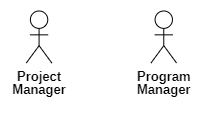
\includegraphics[width=0.3\columnwidth]{usecase/attori} 
    \caption{Attori}
\end{figure}
Gli attori che possiamo trovare all'interno dei casi d'uso rappresentano due risorse aziendali:
\subsubsection*{Project Manager}
Conosciuto come il "Responsabile di Progetto", si occupa dell'avvio, pianificazione ,esecuzione e controllo di un singolo progetto, seguendo tecniche di project management.\\
Le sue principali responsabilità sono:
\begin{itemize}
\item assicurarsi che i progetti siano allineati con gli obiettivi aziendali;
\item coordinare le risorse umane, assicurandosi che vengano utilizzate in modo efficiente;
\item stabilisce milestone, scadenze e obiettivi, monitorando lo stato di avanzamento dei progetti;
\item comunica con stakeholder, team di progetto e altre parti interessate.
\end{itemize}
\subsubsection*{Program Manager}
È un ruolo di gestione all'interno di un'organizzazione, ed è responsabile della pianificazione complessiva e del controllo di più progetti che compongono il suo programma. Collabora strettamente col Project Manager ed i loro compiti spesso si sovrappongono ma differiscono di portata, in quanto il Program Manager supervisiona gruppi di progetti gestiti singolarmente dai Project Manager.

\section{Casi d'uso}

\subsection{Scenario Anagrafiche}
\begin{figure}[H] 
    \centering 
    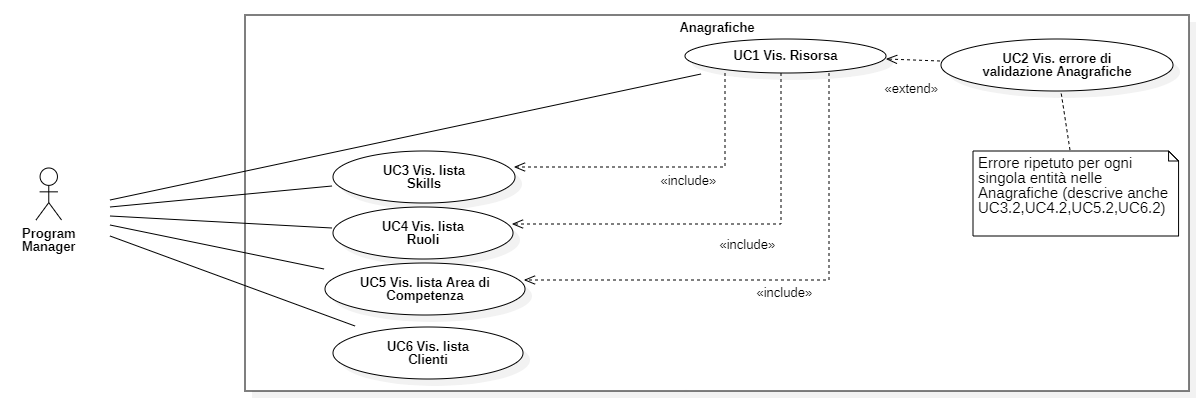
\includegraphics[width=1.1\columnwidth]{usecase/anagrafiche-general} 
    \caption{Casi d'Uso del scenario Anagrafiche}
\end{figure}

\subsubsection*{UC1 - Vis. Risorsa}

\begin{figure}[H] 
    \centering 
    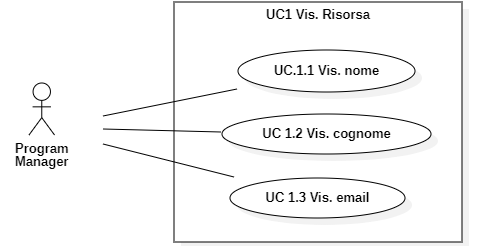
\includegraphics[width=0.6\columnwidth]{usecase/UC1} 
    \caption{Caso d'Uso 1 espanso}
\end{figure}

\begin{itemize}[label=$\circ$]
\item \textbf{Attore:} Program Manager;
\item \textbf{Descrizione:} il Program Manager può visualizzare una Risorsa;
\item \textbf{Precondizioni:} il richiedente è un Program Manager;
\item \textbf{Postcondizioni:} la Risorsa selezionata è visualizzabile dal Program Manager;
\item \textbf{Estensioni:} UC2;
\item \textbf{Inclusioni:} UC3, UC4, UC5.
\end{itemize}

\subsubsection*{UC1.1 - Vis. nome}
\begin{itemize}[label=$\circ$]
\item \textbf{Attore:} Program Manager;
\item \textbf{Descrizione:} il Program Manager può visualizzare il nome di una Risorsa;
\item \textbf{Precondizioni:} la Risorsa è visualizzabile dal Program Manager;
\item \textbf{Postcondizioni:} il Program Manager può visualizzare il nome della Risorsa selezionata;
\item \textbf{Estensioni:} il caso d'uso non ha estensioni;
\item \textbf{Inclusioni:} il caso d'uso non ha inclusioni.
\end{itemize}

\subsubsection*{UC1.2 - Vis. cognome}
\begin{itemize}[label=$\circ$]
\item \textbf{Attore:} Program Manager;
\item \textbf{Descrizione:} il Program Manager può visualizzare il cognome di una Risorsa;
\item \textbf{Precondizioni:}  la Risorsa è visualizzabile dal Program Manager;
\item \textbf{Postcondizioni:} il Program Manager può visualizzare il cognome della Risorsa selezionata;
\item \textbf{Estensioni:} il caso d'uso non ha estensioni;
\item \textbf{Inclusioni:} il caso d'uso non ha inclusioni.
\end{itemize}

\subsubsection*{UC1.3 - Vis. email}
\begin{itemize}[label=$\circ$]
\item \textbf{Attore:} Program Manager;
\item \textbf{Descrizione:} il Program Manager può visualizzare l'email di una Risorsa;
\item \textbf{Precondizioni:}  la Risorsa è visualizzabile dal Program Manager;
\item \textbf{Postcondizioni:} il Program Manager può visualizzare l'email della Risorsa selezionata;
\item \textbf{Estensioni:} il caso d'uso non ha estensioni;
\item \textbf{Inclusioni:} il caso d'uso non ha inclusioni.
\end{itemize}

\subsubsection*{UC2 - Vis. errore di validazione Anagrafiche}
\begin{itemize}[label=$\circ$]
\item \textbf{Attore:} Program Manager;
\item \textbf{Descrizione:} questo caso d'uso descrive anche UC3.2,UC4.2,UC5.2,UC6.2. Viene visualizzato un messaggio di errore in caso vengano eseguite funzionalità con dati non validi. Esso rappresenta errori di validazione nella richiesta fornita dall'utilizzatore;
\item \textbf{Precondizioni:} il Program Manager sta effettuando operazioni con dati non validi;
\item \textbf{Postcondizioni:} l'esecuzione della funzionalità è interrotta e viene visualizzato il messaggio di errore;
\item \textbf{Estensioni:} il caso d'uso non ha estensioni;
\item \textbf{Inclusioni:} il caso d'uso non ha inclusioni.
\end{itemize}

\subsubsection*{UC3 - Vis. lista Skill}
\begin{figure}[H] 
    \centering 
    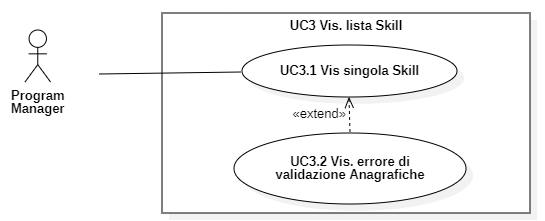
\includegraphics[width=0.6\columnwidth]{usecase/UC3} 
    \caption{Caso d'Uso 3 espanso}
\end{figure}
\begin{itemize}[label=$\circ$]
\item \textbf{Attore:} Program Manager;
\item \textbf{Descrizione:} il Program Manager può visualizzare la lista delle Skill;
\item \textbf{Precondizioni:} il richiedente è un Program Manager;
\item \textbf{Postcondizioni:} la lista delle Skill è visualizzabile dal Program Manager;
\item \textbf{Estensioni:} il caso d'uso non ha estensioni;
\item \textbf{Inclusioni:} il caso d'uso non ha inclusioni.
\end{itemize}

\subsubsection*{UC3.1 - Vis. singola Skill}
\begin{figure}[H] 
    \centering 
    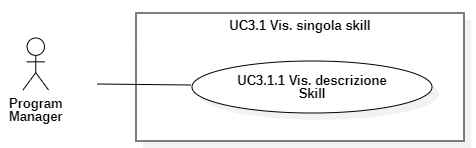
\includegraphics[width=0.6\columnwidth]{usecase/UC3.1} 
    \caption{Caso d'Uso 3.1 espanso}
\end{figure}
\begin{itemize}[label=$\circ$]
\item \textbf{Attore:} Program Manager;
\item \textbf{Descrizione:} il Program Manager può visualizzare una Skill;
\item \textbf{Precondizioni:} il richiedente è un Program Manager;
\item \textbf{Postcondizioni:} la Skill selezionata è visualizzabile dal Program Manager;
\item \textbf{Estensioni:} UC3.2;
\item \textbf{Inclusioni:} il caso d'uso non ha inclusioni.
\end{itemize}

\subsubsection*{UC3.1.1 - Vis. descrizione Skill}
\begin{itemize}[label=$\circ$]
\item \textbf{Attore:} Program Manager;
\item \textbf{Descrizione:} il Program Manager può visualizzare la descrizione di una Skill;
\item \textbf{Precondizioni:} la Skill è visualizzabile dal Program Manager;
\item \textbf{Postcondizioni:} il Program Manager può visualizzare la descrizione della Skill selezionata;
\item \textbf{Estensioni:} il caso d'uso non ha estensioni;
\item \textbf{Inclusioni:} il caso d'uso non ha inclusioni.
\end{itemize}

\subsubsection*{UC4 - Vis. lista Ruoli}
\begin{figure}[H] 
    \centering 
    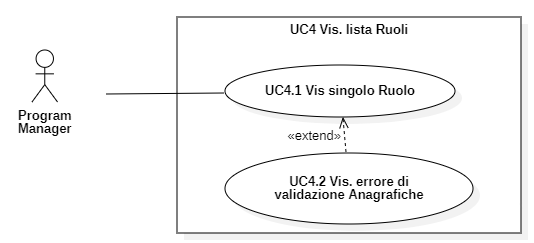
\includegraphics[width=0.6\columnwidth]{usecase/UC4} 
    \caption{Caso d'Uso 4 espanso}
\end{figure}
\begin{itemize}[label=$\circ$]
\item \textbf{Attore:} Program Manager;
\item \textbf{Descrizione:} il Program Manager può visualizzare la lista dei Ruoli;
\item \textbf{Precondizioni:} il richiedente è un Program Manager;
\item \textbf{Postcondizioni:} la lista dei Ruoli è visualizzabile dal Program Manager;
\item \textbf{Estensioni:} il caso d'uso non ha estensioni;
\item \textbf{Inclusioni:} il caso d'uso non ha inclusioni.
\end{itemize}

\subsubsection*{UC4.1 - Vis. singolo Ruolo}
\begin{figure}[H] 
    \centering 
    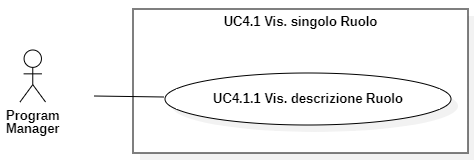
\includegraphics[width=0.6\columnwidth]{usecase/UC4.1} 
    \caption{Caso d'Uso 4.1 espanso}
\end{figure}
\begin{itemize}[label=$\circ$]
\item \textbf{Attore:} Program Manager;
\item \textbf{Descrizione:} il Program Manager può visualizzare un Ruolo;
\item \textbf{Precondizioni:} il richiedente è un Program Manager;
\item \textbf{Postcondizioni:} il Ruolo selezionato è visualizzabile dal Program Manager;
\item \textbf{Estensioni:}  UC4.2;
\item \textbf{Inclusioni:} il caso d'uso non ha inclusioni.
\end{itemize}

\subsubsection*{UC4.1.1 - Vis. descrizione Ruolo}
\begin{itemize}[label=$\circ$]
\item \textbf{Attore:} Program Manager;
\item \textbf{Descrizione:} il Program Manager può visualizzare la descrizione di un Ruolo;
\item \textbf{Precondizioni:}  il Ruolo è visualizzabile dal Program Manager;
\item \textbf{Postcondizioni:} il Program Manager può visualizzare la descrizione del Ruolo selezionato;
\item \textbf{Estensioni:} il caso d'uso non ha estensioni;
\item \textbf{Inclusioni:} il caso d'uso non ha inclusioni.
\end{itemize}

\subsubsection*{UC5 - Vis. lista Area di Competenza}
\begin{figure}[H] 
    \centering 
    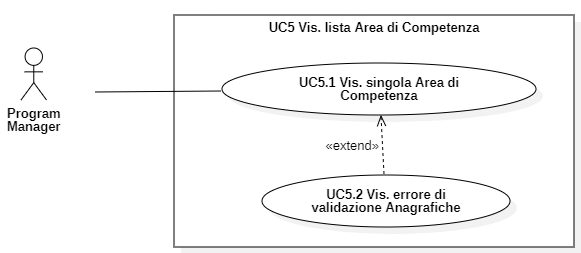
\includegraphics[width=0.6\columnwidth]{usecase/UC5} 
    \caption{Caso d'Uso 5 espanso}
\end{figure}
\begin{itemize}[label=$\circ$]
\item \textbf{Attore:} Program Manager;
\item \textbf{Descrizione:} il Program Manager può visualizzare la lista delle Aree di Competenza;
\item \textbf{Precondizioni:} il richiedente è un Program Manager;
\item \textbf{Postcondizioni:} la lista delle Aree di Competenza è visualizzabile dal Program Manager;
\item \textbf{Estensioni:} il caso d'uso non ha estensioni;
\item \textbf{Inclusioni:} il caso d'uso non ha inclusioni.
\end{itemize}

\subsubsection*{UC5.1 - Vis. singola Area di Competenza}
\begin{figure}[H] 
    \centering 
    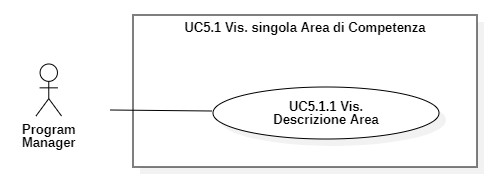
\includegraphics[width=0.6\columnwidth]{usecase/UC5.1} 
    \caption{Caso d'Uso 5.1 espanso}
\end{figure}
\begin{itemize}[label=$\circ$]
\item \textbf{Attore:} Program Manager;
\item \textbf{Descrizione:} il Program Manager può visualizzare un'Area di Competenza;
\item \textbf{Precondizioni:} il richiedente è un Program Manager;
\item \textbf{Postcondizioni:} l'Area di Competenza selezionata è visualizzabile dal Program Manager;
\item \textbf{Estensioni:}  UC5.2;
\item \textbf{Inclusioni:} il caso d'uso non ha inclusioni.
\end{itemize}

\subsubsection*{UC5.1.1 - Vis. descrizione Area}
\begin{itemize}[label=$\circ$]
\item \textbf{Attore:} Program Manager;
\item \textbf{Descrizione:} il Program Manager può visualizzare la descrizione di un'Area di Competenza;
\item \textbf{Precondizioni:}  l'Area è visualizzabile dal Program Manager;
\item \textbf{Postcondizioni:} il Program Manager può visualizzare la descrizione dell'Area di Competenza selezionata;
\item \textbf{Estensioni:} non ci sono estensioni;
\item \textbf{Inclusioni:} non ci sono inclusioni.
\end{itemize}

\subsubsection*{UC6 - Vis. lista Clienti}
\begin{figure}[H] 
    \centering 
    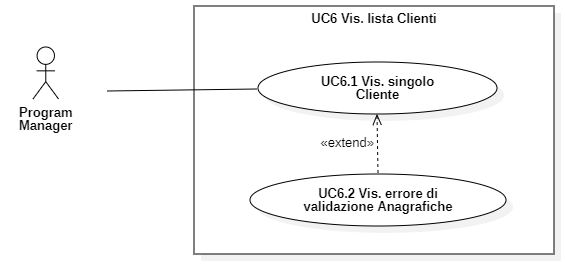
\includegraphics[width=0.6\columnwidth]{usecase/UC6} 
    \caption{Caso d'Uso 6 espanso}
\end{figure}
\begin{itemize}[label=$\circ$]
\item \textbf{Attore:} Program Manager;
\item \textbf{Descrizione:} il Program Manager può visualizzare la lista dei Clienti;
\item \textbf{Precondizioni:} il richiedente è un Program Manager;
\item \textbf{Postcondizioni:} la lista dei Clienti è visualizzabile dal Program Manager;
\item \textbf{Estensioni:} il caso d'uso non ha estensioni;
\item \textbf{Inclusioni:} il caso d'uso non ha inclusioni.
\end{itemize}

\subsubsection*{UC6.1 - Vis. singolo Cliente}
\begin{figure}[H] 
    \centering 
    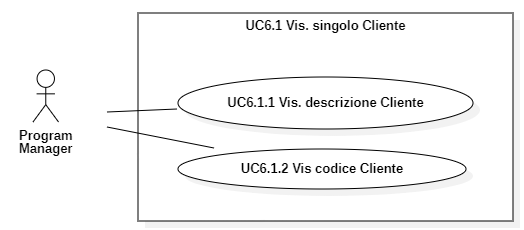
\includegraphics[width=0.6\columnwidth]{usecase/UC6.1} 
    \caption{Caso d'Uso 6.1 espanso}
\end{figure}
\begin{itemize}[label=$\circ$]
\item \textbf{Attore:} Program Manager;
\item \textbf{Descrizione:} il Program Manager può visualizzare un Cliente;
\item \textbf{Precondizioni:} il richiedente è un Program Manager;
\item \textbf{Postcondizioni:} il Cliente selezionato è visualizzabile dal Program Manager;
\item \textbf{Estensioni:} UC6.2;
\item \textbf{Inclusioni:} non ci sono inclusioni.
\end{itemize}

\subsubsection*{UC6.1.1 - Vis. descrizione Cliente}
\begin{itemize}[label=$\circ$]
\item \textbf{Attore:} Program Manager;
\item \textbf{Descrizione:} il Program Manager può visualizzare la descrizione di Cliente;
\item \textbf{Precondizioni:}  il Cliente è visualizzabile dal Program Manager;
\item \textbf{Postcondizioni:} il Program Manager può visualizzare la descrizione del Cliente selezionato;
\item \textbf{Estensioni:} il caso d'uso non ha estensioni;
\item \textbf{Inclusioni:} il caso d'uso non ha inclusioni.
\end{itemize}

\subsubsection*{UC6.1.2 - Vis. codice Cliente}
\begin{itemize}[label=$\circ$]
\item \textbf{Attore:} Program Manager;
\item \textbf{Descrizione:} il Program Manager può visualizzare il codice del Cliente;
\item \textbf{Precondizioni:} il Cliente è visualizzabile dal Program Manager;
\item \textbf{Postcondizioni:} il Program Manager può visualizzare il codice del Cliente selezionato;
\item \textbf{Estensioni:} il caso d'uso non ha estensioni;
\item \textbf{Inclusioni:} il caso d'uso non ha inclusioni.
\end{itemize}


\subsection{Scenario Richieste}
\begin{figure}[H] 
    \centering 
    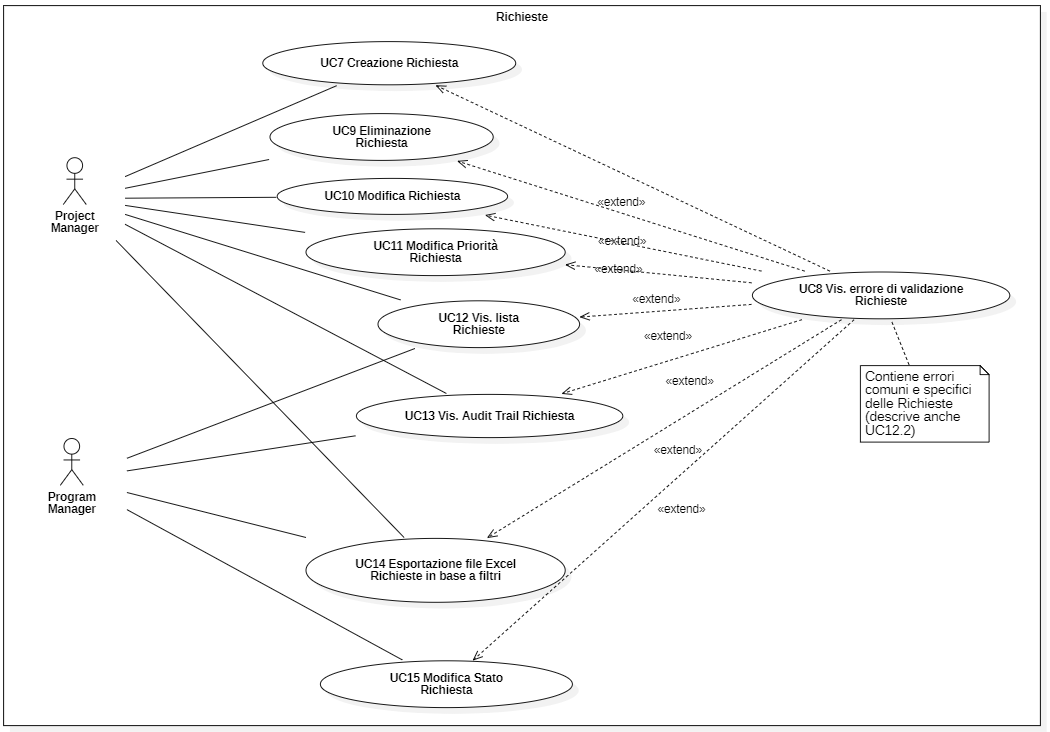
\includegraphics[width=1.1\columnwidth]{usecase/richieste-general} 
    \caption{Casi d'Uso del scenario Richieste}
\end{figure}

\subsubsection*{UC7 - Creazione Richiesta}
\begin{itemize}[label=$\circ$]
\item \textbf{Attore:} Project Manager;
\item \textbf{Descrizione:} il Project Manager può creare una nuova Richiesta;
\item \textbf{Precondizioni:} il richiedente è un Project Manager;
\item \textbf{Postcondizioni:} la Richiesta è stata creata dal Project Manager con successo;
\item \textbf{Estensioni:} UC8;
\item \textbf{Inclusioni:} il caso d'uso non ha inclusioni.
\end{itemize}

\subsubsection*{UC8 - Vis. errore di validazione Richieste}
\begin{itemize}[label=$\circ$]
\item \textbf{Attore:} Project Manager e Program Manager;
\item \textbf{Descrizione:}  questo caso d'uso descrive anche UC12.2. Viene visualizzato un messaggio di errore in caso vengano eseguite funzionalità con dati non validi. Esso rappresenta i seguenti errori comuni all'interno delle Richieste: dati non validi, filtri non valorizzati, entità associate non valide, risultati nulli o non valorizzati;
\item \textbf{Precondizioni:} il Program Manger o il Project Manager stanno effettuando operazioni con dati non validi;
\item \textbf{Postcondizioni:} l'esecuzione della funzionalità è interrotta e viene visualizzato il messaggio di errore;
\item \textbf{Estensioni:} il caso d'uso non ha estensioni;
\item \textbf{Inclusioni:} il caso d'uso non ha inclusioni.
\end{itemize}

\subsubsection*{UC9 - Eliminazione Richiesta}
\begin{itemize}[label=$\circ$]
\item \textbf{Attore:} Project Manager;
\item \textbf{Descrizione:} il Project Manager può eliminare una Richiesta esistente;
\item \textbf{Precondizioni:} il richiedente è un Project Manager;
\item \textbf{Postcondizioni:} la Richiesta è stata eliminata dal Project Manager con successo;
\item \textbf{Estensioni:} UC8;
\item \textbf{Inclusioni:} il caso d'uso non ha inclusioni.
\end{itemize}

\subsubsection*{UC10 - Modifica Richiesta}
\begin{itemize}[label=$\circ$]
\item \textbf{Attore:} Project Manager;
\item \textbf{Descrizione:} il Project Manager può modificare una Richiesta esistente nella sua totalità sovrascrivendola;
\item \textbf{Precondizioni:} il richiedente è un Project Manager;
\item \textbf{Postcondizioni:} la Richiesta selezionata è stata modificata con successo;
\item \textbf{Estensioni:} UC8;
\item \textbf{Inclusioni:} il caso d'uso non ha inclusioni.
\end{itemize}

\subsubsection*{UC11 - Modifica Priorità Richiesta}
\begin{itemize}[label=$\circ$]
\item \textbf{Attore:} Project Manager;
\item \textbf{Descrizione:} il Project Manager può modificare l'attributo Priorità di una Richiesta esistente inserendo un valore tra: Alta, Media o Bassa;
\item \textbf{Precondizioni:} il richiedente è un Project Manager;
\item \textbf{Postcondizioni:} la Richiesta è stata modificata con successo solo nel campo Priorità dal Project Manager;
\item \textbf{Estensioni:} UC8;
\item \textbf{Inclusioni:} il caso d'uso non ha inclusioni.
\end{itemize}

\subsubsection*{UC12 - Vis. lista Richieste}

\begin{figure}[H] 
    \centering 
    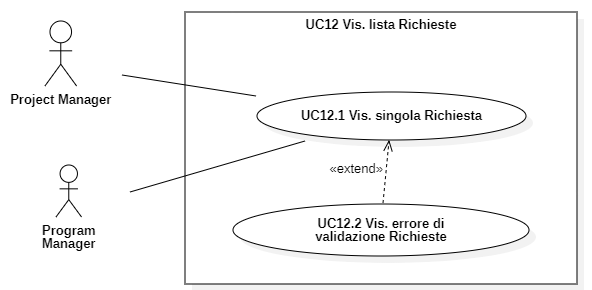
\includegraphics[width=0.6\columnwidth]{usecase/UC12} 
    \caption{Caso d'Uso 12 espanso}
\end{figure}

\begin{itemize}[label=$\circ$]
\item \textbf{Attore:} Project Manager e Program Manager;
\item \textbf{Descrizione:} il Project Manager e il Program Manager possono visualizzare una lista di Richieste dopo aver inserito filtri e/o una parola nella ricerca rapida e aver selezionato se i filtri applicati devono essere congiunti o disgiunti;
\item \textbf{Precondizioni:} il richiedente è un Project Manager o un Program Manager;
\item \textbf{Postcondizioni:} la lista delle Richieste è visualizzabile dal Project Manager e dal Program Manager;
\item \textbf{Estensioni:} UC8;
\item \textbf{Inclusioni:} il caso d'uso non ha inclusioni.
\end{itemize}

\subsubsection*{UC12.1 - Vis. singola Richiesta}

\begin{figure}[H] 
    \centering 
    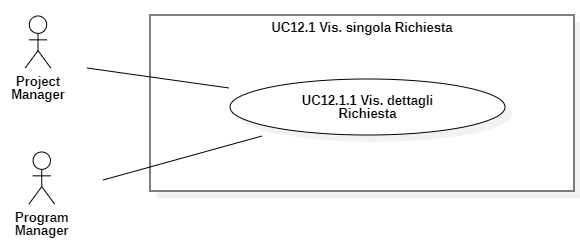
\includegraphics[width=0.6\columnwidth]{usecase/UC12.1} 
    \caption{Caso d'Uso 12.1 espanso}
\end{figure}

\begin{itemize}[label=$\circ$]
\item \textbf{Attore:} Project Manager e Program Manager;
\item \textbf{Descrizione:} il Project Manager e il Program Manager possono visualizzare la Richiesta selezionata;
\item \textbf{Precondizioni:} la lista delle Richieste è visualizzabile;
\item \textbf{Postcondizioni:} la Richiesta selezionata è visualizzabile dal Program Manager e dal Project Manager;
\item \textbf{Estensioni:} UC12.2;
\item \textbf{Inclusioni:} il caso d'uso non ha inclusioni.
\end{itemize}

\subsubsection*{UC12.1.1 - Vis. dettagli Richiesta}

\begin{figure}[H] 
    \centering 
    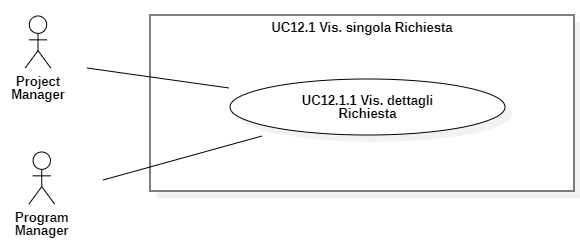
\includegraphics[width=0.6\columnwidth]{usecase/UC12.1} 
    \caption{Caso d'Uso 12.1 espanso}
\end{figure}

\begin{itemize}[label=$\circ$]
\item \textbf{Attore:} Project Manager e Program Manager;
\item \textbf{Descrizione:} il Project Manager e il Program Manager possono visualizzare la Richiesta selezionata;
\item \textbf{Precondizioni:} la Richiesta singola è visualizzabile;
\item \textbf{Postcondizioni:} il Project Manager e il Program Manager possono visualizzare i campi di una Richiesta selezionata;
\item \textbf{Estensioni:} il caso d'uso non ha esclusioni;
\item \textbf{Inclusioni:} il caso d'uso non ha inclusioni.
\end{itemize}

\subsubsection*{UC13 - Vis. audit trail Richiesta}

\begin{figure}[H] 
    \centering 
    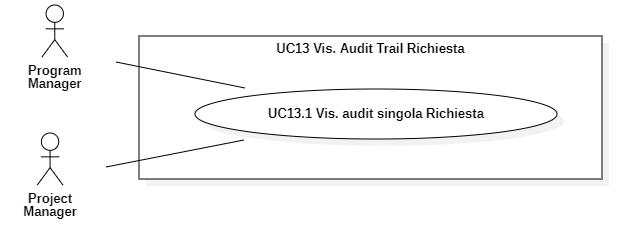
\includegraphics[width=0.6\columnwidth]{usecase/UC13} 
    \caption{Caso d'Uso 13 espanso}
\end{figure}

\begin{itemize}[label=$\circ$]
\item \textbf{Attore:} Project Manager e Program Manager;
\item \textbf{Descrizione:} il Project Manager e il Program Manager possono visualizzare l'audit trail di una Richiesta selezionata.;
\item \textbf{Precondizioni:} il richiedente è un Project Manager o un Program Manager;
\item \textbf{Postcondizioni:} la traccia di audit della Richiesta selezionata è visualizzabile dal Project Manager e dal Program Manager;
\item \textbf{Estensioni:} UC8;
\item \textbf{Inclusioni:} il caso d'uso non ha inclusioni.
\end{itemize}

\subsubsection*{UC13.1 - Vis. audit singola Richiesta}

\begin{figure}[H] 
    \centering 
    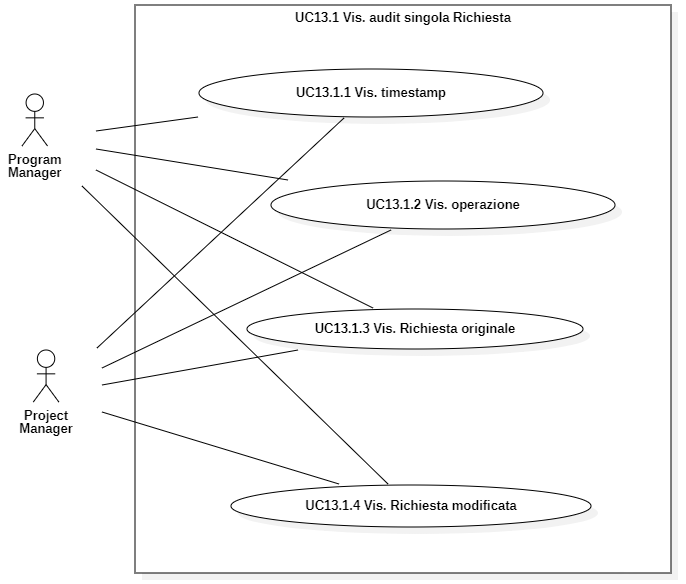
\includegraphics[width=0.8\columnwidth]{usecase/UC13.1} 
    \caption{Caso d'Uso 13.1 espanso}
\end{figure}

\begin{itemize}[label=$\circ$]
\item \textbf{Attore:} Project Manager e Program Manager;
\item \textbf{Descrizione:} il Project Manager e il Program Manager possono visualizzare l'audit di una singola Richiesta;
\item \textbf{Precondizioni:} l'audit trail è visualizzabile;
\item \textbf{Postcondizioni:} l'audit di una singola Richiesta è visualizzabile;
\item \textbf{Estensioni:} il caso d'uso non ha estensioni;
\item \textbf{Inclusioni:} il caso d'uso non ha inclusioni.
\end{itemize}

\subsubsection*{UC13.1.1 - Vis. timestamp}
\begin{itemize}[label=$\circ$]
\item \textbf{Attore:} Project Manager e Program Manager;
\item \textbf{Descrizione:} il Project Manager e il Program Manager possono visualizzare il timestamp di una singola audit di una Richiesta;
\item \textbf{Precondizioni:} la singola audit di una Richiesta è visualizzabile;
\item \textbf{Postcondizioni:} il timestamp della singola audit è visualizzabile;
\item \textbf{Estensioni:} il caso d'uso non ha estensioni;
\item \textbf{Inclusioni:} il caso d'uso non ha inclusioni.
\end{itemize}

\subsubsection*{UC13.1.2 - Vis. operazione}
\begin{itemize}[label=$\circ$]
\item \textbf{Attore:} Project Manager e Program Manager;
\item \textbf{Descrizione:} il Project Manager e il Program Manager possono visualizzare l'operazione di una singola audit di una Richiesta;
\item \textbf{Precondizioni:} la singola audit di una Richiesta è visualizzabile;
\item \textbf{Postcondizioni:} l'operazione della singola audit è visualizzabile;
\item \textbf{Estensioni:} il caso d'uso non ha estensioni;
\item \textbf{Inclusioni:} il caso d'uso non ha inclusioni.
\end{itemize}

\subsubsection*{UC13.1.3 - Vis. Richiesta originale}
\begin{itemize}[label=$\circ$]
\item \textbf{Attore:} Project Manager e Program Manager;
\item \textbf{Descrizione:} il Project Manager e il Program Manager possono visualizzare la singola audit di una Richiesta prima che l'operazione venga eseguita;
\item \textbf{Precondizioni:} la singola audit di una Richiesta è visualizzabile;
\item \textbf{Postcondizioni:} la Richiesta originale della singola audit è visualizzabile;
\item \textbf{Estensioni:} il caso d'uso non ha estensioni;
\item \textbf{Inclusioni:} il caso d'uso non ha inclusioni.
\end{itemize}

\subsubsection*{UC13.1.4 - Vis. Richiesta modificata}
\begin{itemize}[label=$\circ$]
\item \textbf{Attore:} Project Manager e Program Manager;
\item \textbf{Descrizione:} il Project Manager e il Program Manager possono visualizzare la singola audit di una Richiesta dopo che l'operazione è stata eseguita;
\item \textbf{Precondizioni:} la singola audit di una Richiesta è visualizzabile;
\item \textbf{Postcondizioni:} la Richiesta modificata della singola audit è visualizzabile;
\item \textbf{Estensioni:} il caso d'uso non ha estensioni;
\item \textbf{Inclusioni:} il caso d'uso non ha inclusioni.
\end{itemize}

\subsubsection*{UC14 - Esportazione file Excel Richieste in base a filtri}
\begin{itemize}[label=$\circ$]
\item \textbf{Attore:} Project Manager e Program Manager;
\item \textbf{Descrizione:} il Project Manager e il Program Manager possono esportare in un file Excel scaricabile un report delle Richieste in base a dei filtri inseriti;
\item \textbf{Precondizioni:} il richiedente è un Project Manager o un Program Manager;
\item \textbf{Postcondizioni:} il report Excel è stato generato correttamente ed è possibile scaricarlo;
\item \textbf{Estensioni:} UC8;
\item \textbf{Inclusioni:} il caso d'uso non ha inclusioni.
\end{itemize}

\subsubsection*{UC15 - Modifica Stato Richiesta}
\begin{itemize}[label=$\circ$]
\item \textbf{Attore:} Program Manager;
\item \textbf{Descrizione:} il Program Manager può cambiare lo stato di una Richiesta esistente impostandolo in uno dei seguenti valori: Evasa, Non Evasa, Aperta, In corso, Chiusa;
\item \textbf{Precondizioni:} il richiedente è un Program Manager;
\item \textbf{Postcondizioni:} solo lo stato della Richiesta è stato modificato con successo;
\item \textbf{Estensioni:} UC8;
\item \textbf{Inclusioni:} il caso d'uso non ha inclusioni.
\end{itemize}



\subsection{Scenario Pianificazioni}
\begin{figure}[H] 
    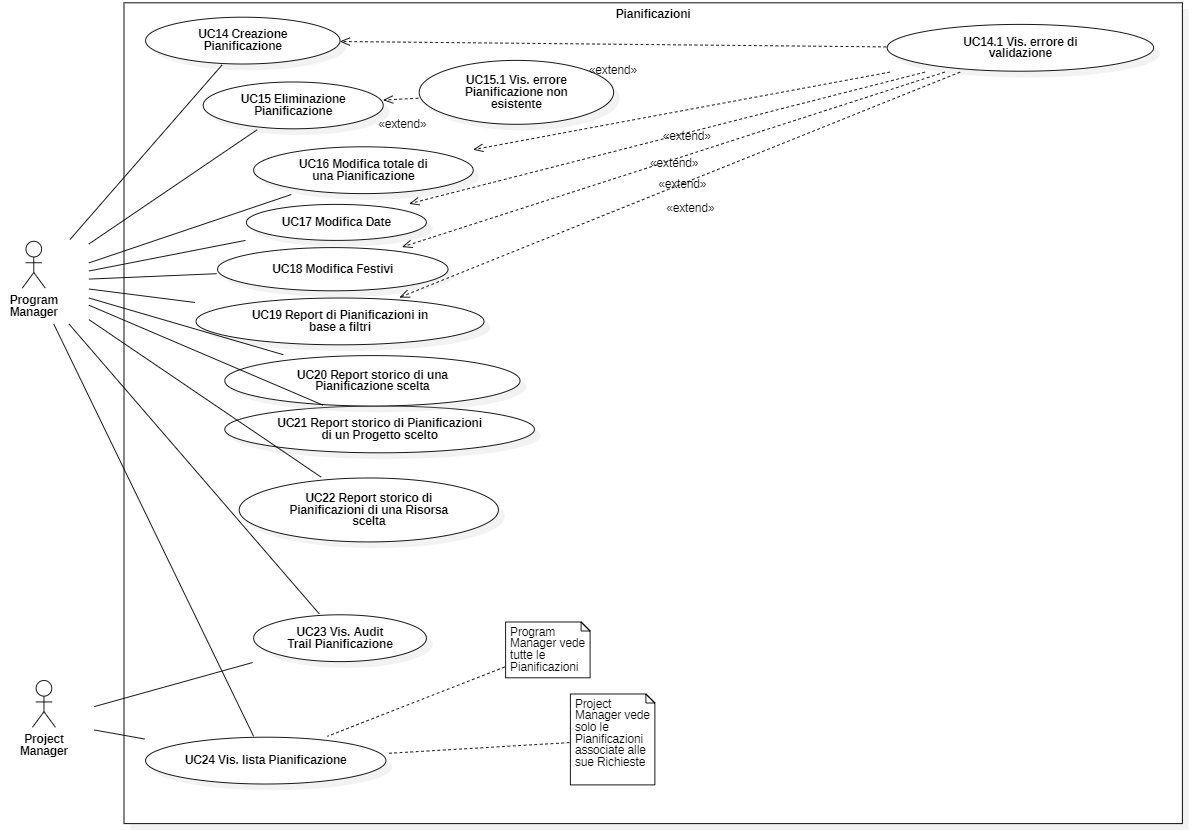
\includegraphics[width=1.00\linewidth]{usecase/pianificazioni-general} 
    \caption{Casi d'Uso del scenario Pianificazioni}
\end{figure}

\subsubsection*{UC16 - Creazione Pianificazione}
\begin{itemize}[label=$\circ$]
\item \textbf{Attore:} Program Manager;
\item \textbf{Descrizione:} il Program Manager può creare una Pianificazione per Figura richiesta da una Richiesta;
\item \textbf{Precondizioni:} il richiedente è un Program Manager;
\item \textbf{Postcondizioni:} la Pianificazione è stata creata dal Program Manager con successo;
\item \textbf{Estensioni:} UC17;
\item \textbf{Inclusioni:} il caso d'uso non ha inclusioni.
\end{itemize}

\subsubsection*{UC17 - Vis. errore di validazione Pianificazioni}
\begin{itemize}[label=$\circ$]
\item \textbf{Attore:} Project Manager e Program Manager;
\item \textbf{Descrizione:} questo caso d'uso descrive anche UC26.2. Viene visualizzato un messaggio di errore in caso vengano eseguite funzionalità con dati non validi. Esso rappresenta i seguenti errori comuni all'interno delle Pianificazioni: dati non validi, filtri non valorizzati, entità associate non valide, risultati nulli o non valorizzati;
\item \textbf{Precondizioni:} il Program Manager o il Project Manager stanno effettuando operazioni con dati non validi;
\item \textbf{Postcondizioni:} l'esecuzione della funzionalità è interrotta e viene visualizzato il messaggio di errore;
\item \textbf{Estensioni:} il caso d'uso non ha estensioni;
\item \textbf{Inclusioni:} il caso d'uso non ha inclusioni.
\end{itemize}

\subsubsection*{UC18 - Eliminazione Pianificazione}
\begin{itemize}[label=$\circ$]
\item \textbf{Attore:} Program Manager;
\item \textbf{Descrizione:} il Program Manager può eliminare una Pianificazione esistente;
\item \textbf{Precondizioni:} il richiedente è il Program Manager;
\item \textbf{Postcondizioni:} la Pianificazione è stata eliminata dal Program Manager con successo;
\item \textbf{Estensioni:} UC17;
\item \textbf{Inclusioni:} il caso d'uso non ha inclusioni.
\end{itemize}

\subsubsection*{UC19 - Modifica Pianificazione}
\begin{itemize}[label=$\circ$]
\item \textbf{Attore:} Program Manager;
\item \textbf{Descrizione:} il Program Manager può modificare una Pianificazione esistente nella sua totalità sovrascrivendola;
\item \textbf{Precondizioni:} il richiedente è un Program Manager;
\item \textbf{Postcondizioni:} la Pianificazione selezionata è stata modificata con successo;
\item \textbf{Estensioni:} UC17;
\item \textbf{Inclusioni:} il caso d'uso non ha inclusioni.
\end{itemize}

\subsubsection*{UC20 - Modifica Date}
\begin{itemize}[label=$\circ$]
\item \textbf{Attore:} Program Manager;
\item \textbf{Descrizione:} il Program Manager può modificare le date di inizio e/o di fine di una Pianificazione;
\item \textbf{Precondizioni:} il richiedente è un Program Manager;
\item \textbf{Postcondizioni:} la Pianificazione è stata modificata con successo solo nel campo Data inizio e/o Data fine dal Program Manager;
\item \textbf{Estensioni:} UC17;
\item \textbf{Inclusioni:} il caso d'uso non ha inclusioni.
\end{itemize}

\subsubsection*{UC21 - Modifica Festivi}
\begin{itemize}[label=$\circ$]
\item \textbf{Attore:} Program Manager;
\item \textbf{Descrizione:} il Porgram Manager può modificare il campo Festivi di una Pianificazione. Se posto a vero il lavoratore potrà lavorare anche nei giorni festivi;
\item \textbf{Precondizioni:} il richiedente è un Program Manager;
\item \textbf{Postcondizioni:}  la Pianificazione è stata modificata con successo solo nel campo Festivi dal Program Manager;
\item \textbf{Estensioni:} UC17;
\item \textbf{Inclusioni:} il caso d'uso non ha inclusioni.
\end{itemize}

\subsubsection*{UC22 - Esportazione file Excel di Pianificazioni in base a filtri}
\begin{itemize}[label=$\circ$]
\item \textbf{Attore:} Program Manager;
\item \textbf{Descrizione:} : il Program Manager può esportare in un
file Excel scaricabile un report delle Pianificazioni in base a dei filtri inseriti;
\item \textbf{Precondizioni:} : il richiedente è un Program Manager;
\item \textbf{Postcondizioni:} il report Excel è stato generato correttamente ed è possibile
scaricarlo;
\item \textbf{Estensioni:} UC17;
\item \textbf{Inclusioni:} il caso d'uso non ha inclusioni.
\end{itemize}

\subsubsection*{UC23 - Esportazione storico Excel di Pianificazioni di un Progetto}
\begin{itemize}[label=$\circ$]
\item \textbf{Attore:} Program Manager;
\item \textbf{Descrizione:} il Program Manager può esportare in un file Excel scaricabile uno storico di Pianificazioni associate ad un Progetto contenente tutte le risorse allocate e l’effettivo impiego di queste nelle attività;
\item \textbf{Precondizioni:} il richiedente è un Program Manager;
\item \textbf{Postcondizioni:} il report Excel è stato generato correttamente ed è possibile
scaricarlo;
\item \textbf{Estensioni:} UC17;
\item \textbf{Inclusioni:} il caso d'uso non ha inclusioni.
\end{itemize}

\subsubsection*{UC24 - Esportazione storico Excel di Pianificazioni di una Risorsa}
\begin{itemize}[label=$\circ$]
\item \textbf{Attore:} Program Manager;
\item \textbf{Descrizione:} il Program Manager può esportare in un file Excel scaricabile uno storico di Pianificazioni in cui c'è stata una determinata Risorsa;
\item \textbf{Precondizioni:} il richiedente è un Program Manager;
\item \textbf{Postcondizioni:} il report Excel è stato generato correttamente ed è possibile
scaricarlo;
\item \textbf{Estensioni:} UC17;
\item \textbf{Inclusioni:} il caso d'uso non ha inclusioni.
\end{itemize}

\subsubsection*{UC25 - Vis. Audit Trail Pianificazione}
\begin{figure}[H] 
    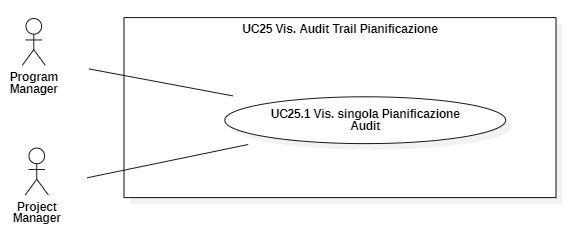
\includegraphics[width=0.65\linewidth]{usecase/UC25} 
    \caption{Caso d'Uso 25 espanso}
\end{figure}

\begin{itemize}[label=$\circ$]
\item \textbf{Attore:} Project Manager o Program Manager;
\item \textbf{Descrizione:} il Project Manager o il Program Manager possono visualizzare
l’audit trail di una Richiesta selezionata. Il Project Manager può vedere solo le tracce di audit delle Pianificazioni associate alle sue Richieste, mentre il Program Manager può vederle tutte;
\item \textbf{Precondizioni:} il richiedente è un Program Manager o un Project Manager;
\item \textbf{Postcondizioni:} la traccia di audit della Pianificazione selezionata è visualizzabile dal Project Manager o dal Program Manager;
\item \textbf{Estensioni:} UC17;
\item \textbf{Inclusioni:} il caso d'uso non ha inclusioni.
\end{itemize}


\subsubsection*{UC25.1 - Vis. singola Pianificazione Audit}
\begin{figure}[H] 
    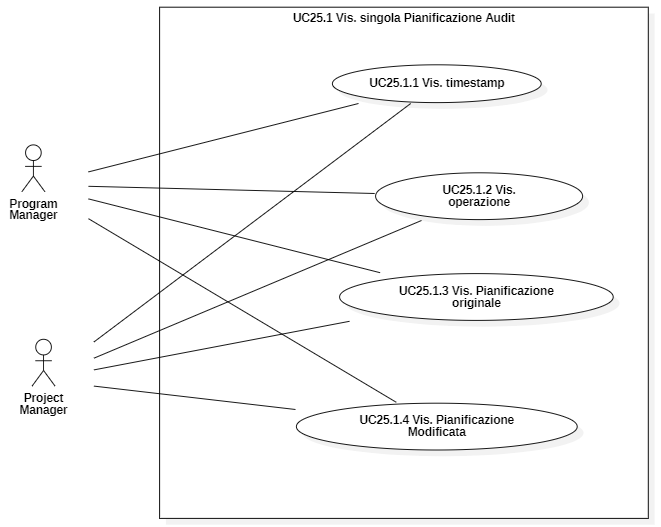
\includegraphics[width=0.75\linewidth]{usecase/UC25.1} 
    \caption{Caso d'Uso 25.1 espanso}
\end{figure}

\begin{itemize}[label=$\circ$]
\item \textbf{Attore:} Project Manager o Program Manager;
\item \textbf{Descrizione:} il Project Manager o il Program Manager può vedere l'audit di una singola Pianificazione. Il Project Manager può vedere solo le Pianificazioni associate alle sue Richieste, mentre il Program Manager può vederle tutte;
\item \textbf{Precondizioni:} l'audit trail è visualizzabile;
\item \textbf{Postcondizioni:} l'audit di una singola Pianificazione è visualizzabile;
\item \textbf{Estensioni:} il caso d'uso non ha estensioni;
\item \textbf{Inclusioni:} il caso d'uso non ha inclusioni.
\end{itemize}

\subsubsection*{UC25.1.1 - Vis. timestamp}

\begin{itemize}[label=$\circ$]
\item \textbf{Attore:} Project Manager o Program Manager;
\item \textbf{Descrizione:} il Project Manager e il Program Manager possono visualizzare il
timestamp di una singola audit di una Pianificazione;
\item \textbf{Precondizioni:} la singola audit di una Pianificazione è visualizzabile;
\item \textbf{Postcondizioni:} il timestamp della singola audit è visualizzabile;
\item \textbf{Estensioni:} il caso d'uso non ha estensioni;
\item \textbf{Inclusioni:} il caso d'uso non ha inclusioni.
\end{itemize}

\subsubsection*{UC25.1.2 - Vis. operazione}

\begin{itemize}[label=$\circ$]
\item \textbf{Attore:} Project Manager o Program Manager;
\item \textbf{Descrizione:} il Project Manager e il Program Manager possono visualizzare l'operazione di una singola audit di una Pianificazione;
\item \textbf{Precondizioni:} la singola audit di una Pianificazione è visualizzabile;
\item \textbf{Postcondizioni:} l’operazione della singola audit è visualizzabile;
\item \textbf{Estensioni:} il caso d'uso non ha estensioni;
\item \textbf{Inclusioni:} il caso d'uso non ha inclusioni.
\end{itemize}

\subsubsection*{UC25.1.3 - Vis. Pianificazione originale}

\begin{itemize}[label=$\circ$]
\item \textbf{Attore:} Project Manager o Program Manager;
\item \textbf{Descrizione:} il Project Manager o il Program Manager possono visualizzare la
singola audit di una Pianificazione prima che l’operazione venga eseguita;
\item \textbf{Precondizioni:}la singola audit di una Pianificazione è visualizzabile;
\item \textbf{Postcondizioni:} la Richiesta originale della singola audit è visualizzabile;
\item \textbf{Estensioni:} il caso d'uso non ha estensioni;
\item \textbf{Inclusioni:} il caso d'uso non ha inclusioni.
\end{itemize}

\subsubsection*{UC25.1.4 - Vis. Pianificazione modificata}

\begin{itemize}[label=$\circ$]
\item \textbf{Attore:} Project Manager o Program Manager;
\item \textbf{Descrizione:} il Project Manager o il Program Manager possono visualizzare la
singola audit di una Pianificazione dopo che l’operazione è stata eseguita;
\item \textbf{Precondizioni:} la singola audit di una Pianificazione è visualizzabile;
\item \textbf{Postcondizioni:} la Pianificazione modificata della singola audit è visualizzabile;
\item \textbf{Estensioni:} il caso d'uso non ha estensioni;
\item \textbf{Inclusioni:} il caso d'uso non ha inclusioni.
\end{itemize}

\subsubsection*{UC26 - Vis. lista Pianificazione}
\begin{figure}[H] 
    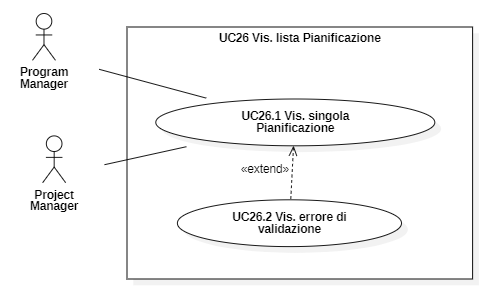
\includegraphics[width=0.65\linewidth]{usecase/UC26} 
    \caption{Caso d'Uso 26 espanso}
\end{figure}

\begin{itemize}[label=$\circ$]
\item \textbf{Attore:}  Project Manager o Program Manager;
\item \textbf{Descrizione:} il Project Manager o il Program Manager possono visualizzare
una lista di Richieste dopo aver inserito filtri e/o una parola nella ricerca rapida
e aver selezionato se i filtri applicati devono essere congiunti o disgiunti. Il Project Manager può vedere solo le Pianificazioni associate alle sue Richieste, mentre il Program Manager può vederle tutte;
\item \textbf{Precondizioni:} il richiedente è un Project Manager o un Program Manager;
\item \textbf{Postcondizioni:} la lista delle Richieste è visualizzabile dal Project Manager o dal Program Manager;
\item \textbf{Estensioni:} UC17;
\item \textbf{Inclusioni:} il caso d'uso non ha inclusioni.
\end{itemize}


\subsubsection*{UC26.1 - Vis. singola Pianificazione}
\begin{figure}[H] 
    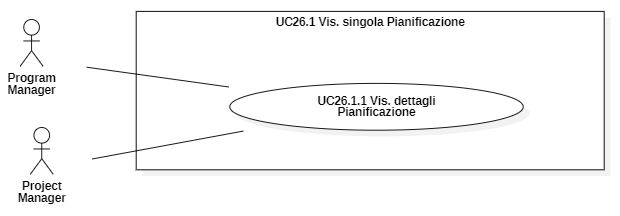
\includegraphics[width=0.75\linewidth]{usecase/UC26.1} 
    \caption{Caso d'Uso 26.1 espanso}
\end{figure}

\begin{itemize}[label=$\circ$]
\item \textbf{Attore:}  Project Manager o Program Manager;
\item \textbf{Descrizione:} il Project Manager o il Program Manager possono visualizzare la Pianificazione selezionata. Il Project Manager può vedere solo le Pianificazioni associate alle sue Richieste, mentre il Program Manager può vederle tutte;
\item \textbf{Precondizioni:} la lista delle Pianificazioni è visualizzabile;
\item \textbf{Postcondizioni:} la Pianificazione selezionata è visualizzabile dal Program Manager o dal Project Manager;
\item \textbf{Estensioni:} UC26.2;
\item \textbf{Inclusioni:} il caso d'uso non ha inclusioni.
\end{itemize}

\subsubsection*{UC26.1.1 - Vis. dettagli Pianificazione}
\begin{itemize}[label=$\circ$]
\item \textbf{Attore:}  Project Manager o Program Manager;
\item \textbf{Descrizione:} il Project Manager o il Program Manager possono visualizzare la
Pianificazione selezionata;
\item \textbf{Precondizioni:} la Pianificazione singola è visualizzabile;
\item \textbf{Postcondizioni:} il Project Manager e il Program Manager possono visualizzare
i campi di una Pianificazione selezionata;
\item \textbf{Estensioni:} il caso d'uso non ha estensioni;
\item \textbf{Inclusioni:} il caso d'uso non ha inclusioni.
\end{itemize}




\subsection{Scenario Milestone}
\begin{figure}[H] 
    \centering 
    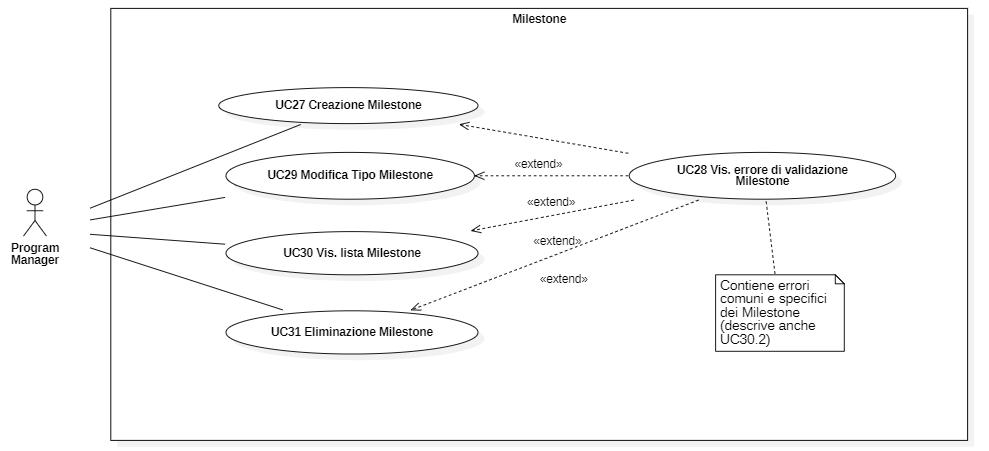
\includegraphics[width=1.05\columnwidth]{usecase/milestone-general} 
    \caption{Casi d'Uso del scenario Milestone}
\end{figure}

\subsubsection*{UC27 - Creazione Milestone}
\begin{itemize}[label=$\circ$]
\item \textbf{Attore:} Program Manager;
\item \textbf{Descrizione:} il Program Manager può creare una nuova Milestone da associare ad una Pianificazione;
\item \textbf{Precondizioni:} il richiedente è un Program Manager;
\item \textbf{Postcondizioni:} la Milestone è stata creata dal Program Manager con successo;
\item \textbf{Estensioni:} UC28;
\item \textbf{Inclusioni:} il caso d'uso non ha inclusioni.
\end{itemize}

\subsubsection*{UC28 - Vis. errore di validazione Milestone}
\begin{itemize}[label=$\circ$]
\item \textbf{Attore:} Program Manager;
\item \textbf{Descrizione:} questo caso d'uso descrive anche UC30.2. Viene visualizzato un messaggio di errore in caso vengano eseguite funzionalità con dati non validi. Esso rappresenta i seguenti errori comuni all'interno delle Milestone: dati non validi, filtri non valorizzati, entità associate non valide, risultati nulli o non valorizzati;
\item \textbf{Precondizioni:} il Program Manager sta effettuando operazioni con dati non validi;
\item \textbf{Postcondizioni:} l'esecuzione della funzionalità è interrotta e viene visualizzato il messaggio di errore;
\item \textbf{Estensioni:} il caso d'uso non ha estensioni;
\item \textbf{Inclusioni:} il caso d'uso non ha inclusioni.
\end{itemize}

\subsubsection*{UC29 - Modifica Tipo Milestone}
\begin{itemize}[label=$\circ$]
\item \textbf{Attore:} Program Manager;
\item \textbf{Descrizione:}  il Program Manager può modificare il Tipo di una Milestone in due possibili valori: Alert o Reminder;
\item \textbf{Precondizioni:} il richiedente è un Program Manager;
\item \textbf{Postcondizioni:} la Milestone è stata modificata con successo solo nel campo
Tipo dal Program Manager;
\item \textbf{Estensioni:} UC28;
\item \textbf{Inclusioni:} il caso d'uso non ha inclusioni.
\end{itemize}

\subsubsection*{UC30 - Vis. lista Milestone}
\begin{figure}[H] 
    \centering 
    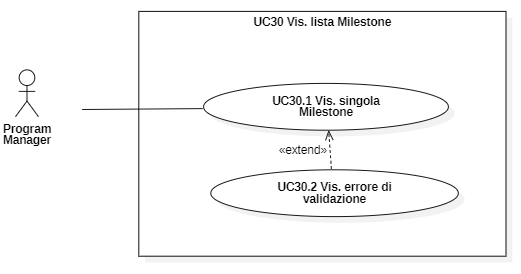
\includegraphics[width=0.70\columnwidth]{usecase/UC30} 
    \caption{Casi d'Uso 30 espanso}
\end{figure}
\begin{itemize}[label=$\circ$]
\item \textbf{Attore:} Program Manager;
\item \textbf{Descrizione:} il Program Manager può visualizzare una lista di Milestone dopo aver inserito filtri e/o una parola nella ricerca rapida e aver selezionato se i filtri applicati devono essere congiunti o disgiunti;
\item \textbf{Precondizioni:} il richiedente è un Program Manager;
\item \textbf{Postcondizioni:} la lista delle Milestone è visualizzabile dal Program Manager;
\item \textbf{Estensioni:} UC28;
\item \textbf{Inclusioni:} il caso d'uso non ha inclusioni.
\end{itemize}

\subsubsection*{UC30.1 - Vis. singola Milestone}
\begin{figure}[H] 
    \centering 
    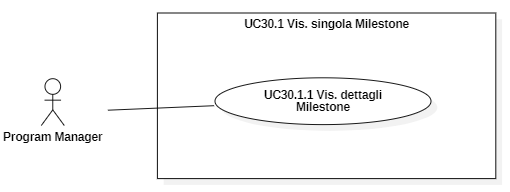
\includegraphics[width=0.70\columnwidth]{usecase/UC30.1} 
    \caption{Casi d'Uso 30.1 espanso}
\end{figure}
\begin{itemize}[label=$\circ$]
\item \textbf{Attore:} Program Manager;
\item \textbf{Descrizione:} il Program Manager può visualizzare la Milestone selezionata;
\item \textbf{Precondizioni:} la lista delle Milestone è visualizzabile;
\item \textbf{Postcondizioni:} la Milestone selezionata è visualizzabile dal Program Manager;
\item \textbf{Estensioni:} UC30.2;
\item \textbf{Inclusioni:} il caso d'uso non ha inclusioni.
\end{itemize}

\subsubsection*{UC30.1.1 - Vis. dettagli Milestone}
\begin{itemize}[label=$\circ$]
\item \textbf{Attore:} Program Manager;
\item \textbf{Descrizione:} il Program Manager può visualizzare la Milestone selezionata;
\item \textbf{Precondizioni:} la Milestone singola è visualizzabile;
\item \textbf{Postcondizioni:} il Project Manager può visualizzare i campi di una Milestone selezionata;
\item \textbf{Estensioni:} il caso d'uso non ha esclusioni;
\item \textbf{Inclusioni:} il caso d'uso non ha inclusioni.
\end{itemize}

\subsubsection*{UC31 - Eliminazione Milestone}
\begin{itemize}[label=$\circ$]
\item \textbf{Attore:} Program Manager;
\item \textbf{Descrizione:} il Program Manager può eliminare una Milestone esistente;
\item \textbf{Precondizioni:} il richiedente è un Program Manager;
\item \textbf{Postcondizioni:} la Milestone è stata eliminata dal Program Manager con successo;
\item \textbf{Estensioni:} UC28;
\item \textbf{Inclusioni:} il caso d'uso non ha inclusioni.
\end{itemize}



\section{Tracciamento dei requisiti}


 


    \chapter{Background tecnologico}
\label{cap:tecnologie}

\section{Scopo del capitolo}
Questo capitolo tratta delle tecnologie e gli strumenti di sviluppo e di supporto utilizzati per la realizzazione del prodotto.\\ L'apprendimento delle seguenti tecnologie e strumenti è stato affrontato nella prima parte del tirocinio. Questo periodo di formazione è durato circa due settimane in cui il tutor mi ha fornito materiale ed esercitazioni per poter comprendere al meglio il contesto tecnologico.\\

\section{Tecnologie}
\subsection*{Java}
Java è un linguaggio di programmazione ad alto livello, orientato agli oggetti e fortemente tipizzato, sviluppato originariamente da Sun Microsystems.\\
La sua popolarità deriva dalla sua portabilità, dalla vasta comunità di sviluppatori e dalle numerose risorse disponibili per l'apprendimento e lo sviluppo.\\
All'interno del mio progetto è stato utilizzato per lo sviluppo del lato back-end del prodotto. 
\\

\subsection*{SQL}
SQL, acronimo di Structured Query Language, è un linguaggio di programmazione utilizzato per gestire e manipolare dati in un database relazionale. SQL fornisce una serie di comandi standardizzati che consentono agli sviluppatori e agli amministratori di database di eseguire operazioni come l'interrogazione dei dati, l'aggiornamento dei dati, l'inserimento di nuovi dati e la creazione e gestione degli schemi dei database.\\
Questo noto linguaggio è stato utilizzato nel progetto per i seguenti motivi:
\begin{itemize}
\item creare le tabelle o trigger utili alla fruizione dei servizi del progetto;
\item eseguire query per inserire, recuperare, eliminare o modificare dati in base alle richieste.
\end{itemize}

\subsection*{Microsoft SQL Server}
SQL Server è un DBMS (Database Management System) relazionale sviluppato da Microsoft. È una piattaforma dati che si utilizza per creare e gestire database, principalmente in ambito aziendale.\\

\subsection*{Spring}
Spring è un framework\textsubscript{g} di sviluppo di applicazioni Java che offre un'ampia gamma di strumenti e librerie per semplificare la creazione di applicazioni aziendali robuste, scalabili e di alta qualità. 
Spring fornisce anche moduli specifici per la gestione dei dati, lo sviluppo web e la sicurezza, rendendolo uno degli strumenti più utilizzati per lo sviluppo Java.\\
A questo framework sono associati tanti altri progetti, che hanno nomi composti come Spring Boot, Spring Data e molti altri.\\
All'interno del progetto Spring è stato utilizzato per sviluppare l'API REST.
\\

\subsection*{Spring Boot}
Spring Boot è un modulo del framework di sviluppo Java Spring che semplifica la creazione, la configurazione e l'avvio di applicazioni Java. Fornisce un ambiente pronto all'uso per sviluppare rapidamente applicazioni Spring, eliminando gran parte della complessità associata alla configurazione. Spring Boot utilizza convenzioni intelligenti e configurazioni predefinite per accelerare lo sviluppo, consentendo agli sviluppatori di concentrarsi sulle funzionalità dell'applicazione anziché sulla configurazione di base.
\\

\subsection*{Spring Data}
Spring Data è un modulo del framework Spring che fornisce un'astrazione per semplificare l'accesso e la gestione dei dati nelle applicazioni Java. Esso offre un'interfaccia unificata per interagire con una varietà di fonti di dati, tra cui database relazionali, database NoSQL e altri servizi di memorizzazione dati.\\
Questo modulo è stato utile nel progetto per interfacciare l'applicazione con il database.
\\

\subsection*{JSON}
JSON, acronimo di JavaScript Object Notation, è un formato leggero di scambio di dati utilizzato comunemente per rappresentare oggetti e strutture di dati.
JSON è ampiamente utilizzato per rappresentare dati in applicazioni web, servizi API, scambio di dati tra client e server, configurazioni di applicazioni e molto altro.\\
All'interno del progetto permette lo scambio di dati tra il lato front-end ed il lato back-end.
\\

\section{Strumenti}
\subsection{Strumenti di sviluppo}
Gli strumenti di sviluppo sono utilizzati direttamente per creare, implementare e testare le funzionalità dell'applicazione. Essi contribuiscono alla realizzazione delle funzionalità dell'applicazione stessa.\\

\subsubsection*{IntelliJ IDEA}
IntelliJ IDEA è un potente ambiente di sviluppo integrato (IDE) sviluppato da JetBrains, progettato principalmente per la programmazione in linguaggi come Java, Kotlin, Scala e altri.
È noto per la sua ricca serie di funzionalità progettate per migliorare l'efficienza degli sviluppatori e semplificare il processo di sviluppo del software.\\
Il seguente IDE è stato utilizzato per la scrittura del codice in Java.\\

\subsubsection*{Maven}
Maven è uno strumento di gestione delle build e delle dipendenze che fornisce un sistema di automazione per la compilazione, il testing, il packaging delle applicazioni e il download delle dipendenze.\\
All'interno di questo progetto Maven è stato utilizzato con Spring Boot per semplificare la gestione delle dipendenze e delle versioni.
\\


\subsubsection*{DBeaver}
DBeaver è un'applicazione di amministrazione di database universale e strumento client SQL. È utilizzato per connettersi, esplorare, gestire e interrogare diversi tipi di database.\\
All'interno del progetto è stato utilizzato per interagire col database.
\\


\subsubsection*{Hibernate}
Hibernate è un framework di mapping\textsubscript{g} oggetto-relazionale (ORM). L'obiettivo principale di Hibernate è semplificare la gestione e l'accesso ai dati in un database relazionale utilizzando oggetti Java anziché scrivere query SQL manualmente.
\\


\subsubsection*{Postman}
Postman è un'applicazione di sviluppo di API (Application Programming Interface) che consente agli sviluppatori di creare, testare, documentare e monitorare le API.\\
Nel corso del progetto è stato uno strumento altamente utilizzato sia come API testing tool.\\

\subsection{Strumenti di supporto}
Gli strumenti di supporto sono utilizzati per attività che sostengono lo sviluppo del progetto. Essi contribuiscono a migliorare la gestione, la qualità e l'efficienza del processo di sviluppo.\\
 
\subsubsection*{Microsoft Teams}
Microsoft Teams è una piattaforma di comunicazione e collaborazione aziendale sviluppata da Microsoft. Offre strumenti per la chat, le videoconferenze, la condivisione di documenti e la gestione dei progetti, consentendo ai team di lavorare insieme in modo efficace sia in ufficio che a distanza.\\
Questa piattaforma è stata utilizzata nel corso del progetto per poter comunicare con il tutor anche quando non era in ufficio o con altri colleghi per determinate situazioni lavorative.


\subsubsection*{Notion}
Notion è un'applicazione di gestione delle informazioni, utilizzata per prendere appunti, creare elenchi di attività, scrivere documenti e molto altro grazie alla sua interfaccia flessibile personalizzabile dagli utenti.\\
Questa applicazione è stata utilizzata nel corso della mia attività di Stage per prendere appunti o tenere traccia delle tasks che dovevo svolgere.\\ 


\subsubsection*{Microsoft Excel}
Microsoft Excel è un'applicazione software di fogli di calcolo sviluppata da Microsoft. È utilizzata per creare, organizzare e analizzare dati in forma di tavole e grafici, offrendo inoltre molte funzionalità per eseguire calcoli.\\
Questa applicazione è stata utilizzata nel progetto allo scopo di velocizzare la creazione di dati fittizi per popolare le tabelle del database per poter testare quanto prodotto.\\


\subsubsection*{Visual Studio Code}
Visual Studio Code è un editor di codice sorgente sviluppato da Microsoft. È progettato per fornire un ambiente di sviluppo leggero, flessibile e personalizzabile per programmatori e sviluppatori.\\
È stato utilizzato nel progetto scaricando varie estensioni per visualizzare l'API e l'UML del database.\\

\subsubsection*{Docker}
Docker è una piattaforma di containerizzazione\textsubscript{g} che consente di creare, distribuire e gestire container\textsubscript{g} virtualizzati\textsubscript{g}. Permette di far funzionare le applicazioni in altri ambienti con facilità.\\
Nel progetto è stato utilizzato per creare un server locale con un'immagine del database MSSQL.\\

\subsubsection*{Swagger}
Swagger è un insieme di strumenti e specifiche che consentono la documentazione, la progettazione e il test di API. Permette una migliore comunicazione dei propri endpoint dell'API semplificandone la lettura e la comprensione.\\

\subsubsection*{Git}
Git è un sistema di controllo versione distribuito utilizzato nello sviluppo software. Consente di tenere traccia delle modifiche apportate al codice sorgente e di semplificare la collaborazione tra sviluppatori in progetti di programmazione.\\


\subsubsection*{GitLab}
GitLab è una piattaforma di sviluppo software basata su web che offre una serie di strumenti per la gestione del ciclo di vita dello sviluppo delle applicazioni. Le principali funzionalità sono: la gestione dei repository Git, la collaborazione tra i membri del team e il monitoraggio delle issue.\\
All'interno del progetto è stato utilizzata come repository per tenere salvato il progresso del progetto. Nella mia attività di stage ho lavorato su un branch a me dedicatomi.\\

\subsubsection*{Git Extensions}
Git Extensions è un'interfaccia grafica per il sistema di controllo versione distribuito Git. Questo software fornisce una modalità visuale per interagire con i repository Git.




    \chapter{Progettazione}
\label{cap:progettazione}

\section{Scopo del capitolo}
In questo capitolo si tratterà dei giorni successivi all'apprendimento del background tecnologico, in cui sono state improntate le basi dell'architettura del progetto, definendo lo schema del database su cui si poggia l'API.\\
Nei seguenti paragrafi verrà quindi trattata l'architettura e le configurazioni utilizzate che funzionano da base per l'implementazione di quanto sviluppato.\\

\section{Architettura REST}
L’architettura REST, acronimo di “Representational State Transfer”, è un approccio di progettazione per la creazione di servizi web che si basa sui principi dell’HTTP (Hypertext Transfer Protocol).\\
Le principali caratteristiche di un’architettura REST includono:
\begin{itemize}
\item \textbf{Sistema client-server}, dove il client è chi fa le richieste e il server fornisce le risposte;
\item \textbf{Sistema layered},perchè possono essere composte da più livelli di servizi indipendenti;
\item \textbf{Stateless}, significa che il server non contiene client state, quindi ogni richiesta ha abbastanza informazione per il server per processarla;
\item \textbf{Cacheable}, significa che l’architettura può memorizzare le risposte dei server e riutilizzarle;
\item \textbf{Resource-based}: questo approccio è considerato tale, dato che si concentra sull’identificazione e la gestione delle risorse all’interno di un sistema. Le risorse vengono identificate da degli URI ed esse possono essere create,aggiornate,richieste o eliminate (operazioni CRUD) attraverso operazioni HTTP standard (POST,PUT,GET,DELETE);
\item \textbf{Manipolazione delle risorse}, poichè le risorse sono diverse dalla loro rappresentazione logica, utilizzando formati come JSON o XML.
\end{itemize}
Questo stile architetturale è utilizzato soprattutto per la realizzazione di API poichè l'adozione dei principi standard di HTTP mantiene un'interfaccia uniforme e l'approccio resource-based ne semplifica la progettazione, dato che le risorse vengono identificate da URI\textsubscript{g}.

\subsection{Convenzioni di denominazione REST}
Buona prassi nella creazione di un'API REST è il rispetto di convenzioni per la nomenclatura degli endpoint\textsubscript{g}. Sebbene non esista un'unica convenzione obbligatoria, esistono delle best practices per garantire una facile lettura e comprensibilità per agevolare gli sviluppatori che adoperano l'API.\\
Le seguenti convenzioni sono state rispettate nella progettazione dell'API:
\begin{itemize}
\item  pluralizzare le risorse, per distinguere se si fa riferimento ad una lista di una determinata risorsa o ad una singola risorsa;
\item usare lettere minuscole;
\item non usare estensioni dei file;
\item in caso di nomi composti utilizzare il "-";
\item non usare underscore;
\item non utilizzare abbreviazioni o slang;
\item non utilizzare verbi, poichè l'azione dovrebbe essere indicata dal metodo HTTP utilizzato.
\end{itemize}

\section{Spring MVC}
Nello sviluppo di una API REST tramite Spring Boot è comune l'utilizzo del pattern architetturale Model-View-Controller(MVC).\\

\begin{figure}[H] 
    \centering 
    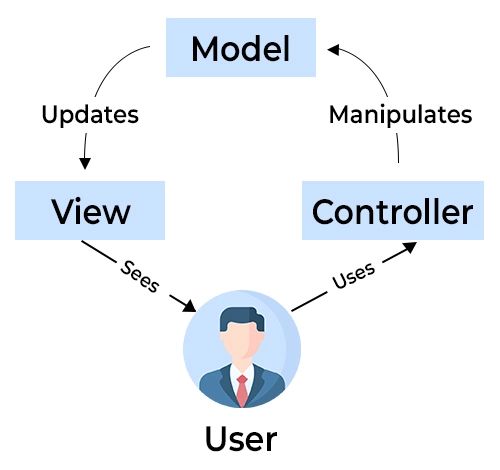
\includegraphics[width=0.50\columnwidth]{mvc2} 
    \caption{Schema Model-View-Controller}
\end{figure}

\subsection{Model}
Il Modello o Model in inglese,appresenta i dati e i metodi per accedere ai dati dell'applicazione. Se esso viene aggiornato in seguito ad azioni o eventi, notificherà la View e il Controller del cambiamento.\\
Nel contesto dello sviluppo di un'API REST, il Model contiene dati che vengono elaborati e restituiti dall'API.\\
All'interno del progetto il Model è formato dai seguenti elementi.
\subsubsection*{Entità}
Le entità sono risorse rappresentate con classi Java segnate con l'annotazione\textsubscript{g} \textit{@Entity}. Utilizzando questa annotazione si identifica che quella classe è mappata\textsubscript{g} ad una tabella del database. Esse dichiarano al loro interno, tramite annotazioni JPA apposite, gli attributi corrispondenti alla tabella a cui fa riferimento e, altre annotazioni per mantenere le relazioni presenti nel database tra le tabelle.
\subsubsection*{Repository}
Le repository implementate nel progetto gestiscono l'accesso ai dati e definiscono metodi per eseguire operazioni di base sui dati, come l'inserimento, la modifica, la cancellazione e la ricerca. Tutto questo estendendo interfacce JPA, che consentono di eseguire operazioni in una base di dati senza scrivere codice SQL o query.
\subsubsection*{DTO}
Data Transfer Object (DTO), oggetti utilizzati per modellare le rappresentazioni dei dati, utilizzati per definire sia i dati inviati dal client nelle requests che quelli che inviati dal server al cliente nelle responses.\\

\subsection{View}
La Vista o View in inglese, è responsabile di mostrare i dati provenienti dal Model e dell'interazione con l'utente. Essa cattura gli input dell'utente e delega al Controller l'elaborazione.\\
Dato che il progetto si concentrava sul lato back-end, precisamente sullo sviluppo dell'API REST, non ho quindi sviluppato una vera e propria View, poichè l'output è in formato JSON. In questo contesto l'output prodotto contenente i dati presentati al client in formato JSON, potrebbe essere considerata come "View".\\

\subsection{Controller}
Il Controller gestisce il flusso dell'applicazione. Esso riceve i comandi dell'utente attraverso la View e reagisce eseguendo operazioni conseguenti. Queste sue operazioni possono o meno coinvolgere il Model, ma portano generalmente sempre ad un cambiamento di stato della View.\\
All'interno del meccanismo di Spring MVC il Controller gestisce le richieste HTTP in arrivo, selezionando il Controller adeguato e assegnato a quell'endpoint API. Sono quindi responsabili di ricevere le richieste, elaborarle e restituire le risposte corrispondenti.\\
Per identificare il metodo associato ad una determinata operazione HTTP, vengono utilizzate le seguenti annotazioni \textit{@PostMapping}, \textit{@GetMapping}, \textit{@PutMapping}, \textit{@PatchMapping} e \textit{@DeleteMapping}. 
All'interno del progetto il Controller è formato dai seguenti elementi.
\subsubsection*{Controller}
I Controller contengono i metodi a cui vengono associati i percorsi delle richieste HTTP. Esso interpreta i parametri che possono provenire dall'URL o dal corpo della richiesta(parametri di query o dati JSON). Internamente a questi metodi viene richiamato il Service appropriato per eseguire operazioni di business logic al risultato finale da restituire.\\
Per garantire che i dati inseriti dagli utenti o provenienti da richieste siano conformi alle aspettative e non causino errori vengono inseriti dei controlli di validazioni all'interno dei metodi del Controller.
\subsubsection*{Service}
I Service eseguono operazioni complesse ed elaborazioni di dati, gestendo la business logic dell'applicazione. Essi interagiscono con i Repository per recuperare dati dal database e vengono richiamati all'interno dei metodi del Controller.
\subsubsection*{Exception Handler}
Per centralizzare la gestione delle eccezioni è stato creato un handler che garantisce uniformità alle eccezioni che l'applicazione può produrre.\\


\section{Pattern Client-Server}
\begin{figure}[H] 
    \centering 
    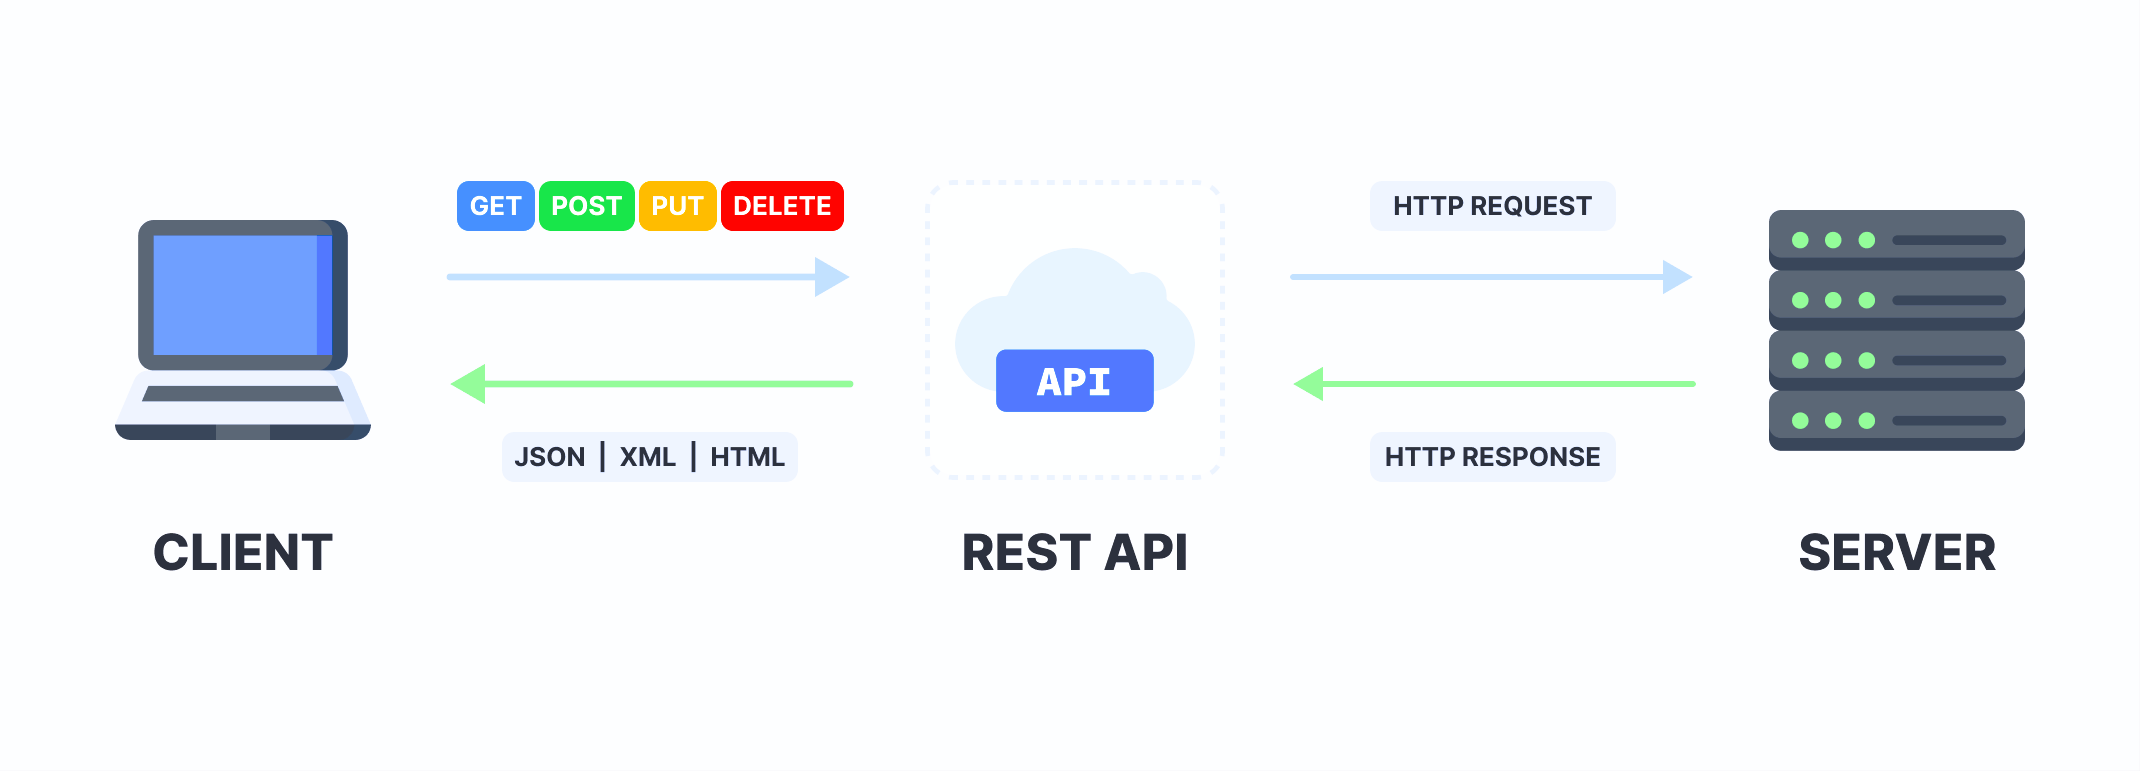
\includegraphics[width=0.90\columnwidth]{client-server} 
    \caption{Client-Server in una REST API}
\end{figure}
È un pattern architetturale composto da due componenti: client e server. Il client rappresenta il richiedente del servizio, mentre il server fornisce i contenuti e i servizi ai client, restando in attesa delle loro richieste.\\
Il pattern client-server si adatta perfettamente ad una API REST e le sue componenti sono identificate in questo modo.
\subsection*{Client}
In questo contesto il client è rappresentato da applicazioni o servizi che comunicano con l'API REST, inviando le richieste HTTP al server per ottenere quanto richiesto. Il client invia richieste utilizzando verbi standard HTTP per accedere alle risorse e alle funzionalità che l'API offre.
\subsection*{Server} 
Il server invece è colui che gestisce le richieste HTTP ricevute e genera le risposte in formato JSON. Esso quindi elabora le richieste ed interagisce col database per recuperare le informazioni.\\

\section{Design Pattern}
\label{cap:design pattern}
Nel prodotto sviluppato possiamo notare i seguenti Design Pattern.
Ad eccezione dell'ultimo Design Pattern adottato, in riferimento all'elenco sottostante, i restanti Design Pattern sono già implementati da Spring e Spring Boot.
\subsection*{Repository pattern}
Repository è un pattern ideato per dividere le operazioni di business logic da quelle di persistenza dei dati. Questo pattern fornisce astrazione ai dati nascondendo i dettagli di accesso, facilita il testing, supporta diverse sorgenti di dati e mantiene un codice riutilizzabile in quanto non sarà necessario modificare ampiamente il codice in caso di modifiche alla sorgente dati.\\
In Spring Boot vengono implementate interfacce annotandole con  l'annotazione \textit{@Repository} ed estendendole con interfacce JPA che permettono l'utilizzo di metodi che forniscono query basilari o la possibilità di creare metodi custom per query personalizzate.
\subsection*{Dependency Injection}
Dependency Injection è un pattern che inietta una dipendenza in una classe senza sapere l'implementazione effettiva. Questo può avvenire attraverso constructor injection, setter injection o method injection. Gli obiettivi di questo pattern sono: eliminare il forte accoppiamento tra le classi, rendere il codice più manutenibile e più facile da testare.\\
In Spring Boot risulta evidente tramite l'utilizzo di annotazioni come \textit{@Autowired}, iniettando direttamente le dipendenze necessarie, promuovendo il concetto successivo di Inversion of Control;
\subsection*{Inversion of Control}
Inversion of Control (IoC) è un design pattern nato sul concetto di invertire il controllo del flusso del sistema nella gestione delle dipendenze e del controllo interno di un'applicazione. Normalmente è l'applicazione che controlla le dipendenze o il flusso di esecuzione, ma questa responsabilità, utilizzando questo pattern, viene trasferita ad un framework. Il framework instanzierà oggetti, inietterà le dipendenze e coordinerà il flusso di esecuzione.\\
Spring Boot è costruito proprio su questo concetto chiave. Esso è correlato a IoC per i seguenti motivi:
\begin{itemize}
\item Component scan, esegue automaticamente uno scan delle classi individuando quelle contrassegnate con annotazioni come \textit{@Service}, \textit{@Repository}, \textit{@Controller} e altre;
\item Semplifica la gestione delle dipendenze, fornendo degli insiemi di dipendenze utili per determinate tecnologie sotto il nome di "starters", velocizzando l'inizializzazione delle dipendenze senza doverle configurare manualmente, fornendo un senso di controllo sulla configurazione iniziale;
\item Dependency Injection;
\item Application Context, agisce come contenitore per i bean\textsubscript{g} dell'applicazione. Esso gestisce i loro cicli di vita e inietta le dipendenze nei punti appropriati.
\end{itemize}
\subsection*{Front Controller}
Il Front Controller è un design pattern che permette di centralizzare la gestione delle richieste all'interno di un'applicazione. In Spring MVC è implementato dal framework per gestire le richieste HTTP verso il Controller adeguato.
\subsection*{Data Transfer Object}
Data Transfer Object (DTO) è un pattern utilizzato per gestire il trasferimento dei dati tra client e server. Gli obiettivi principali del pattern sono:
\begin{itemize}
\item Sicurezza, in quanto puoi controllare cosa si invia;
\item Flessibilità, puoi adattare i DTO in base alle esigenze dell'API;
\item Separano la rappresentazione interna da quella esterna dei dati.
\end{itemize}
Nel contesto di una API REST, i DTO vengono utilizzati sia nella Request che nella Response. Vengono utilizzati in entrambi i punti perchè quando il client invia dei dati magari non necessita degli oggetti completi ma solo di alcune informazioni. Invece quando il server restituisce dei dati il client se li può aspettare sotto una determinata struttura.\\




\section{Progettazione del database}
\subsection{Configurazione di Docker}
I container Docker offrono un'isolamento completo dell'ambiente, che aiuta a evitare conflitti di dipendenze e interferenze con altre applicazioni o servizi che potrebbero essere presenti sul sistema. Per questo motivo si è deciso di utilizzare l'approccio di sandboxing\textsubscript{g} che offre Docker, poichè l'utilizzo di container consente di isolare le applicazioni e i servizi in ambienti virtualizzati, condividendo il kernel del sistema operativo host ma separando le loro risorse e i loro processi.\\
Dato che le tabelle di mia creazione dovevano integrarsi con il database aziendale, tramite il tool Docker Compose\textsubscript{g} e un file di configurazione \textit{docker-compose.yaml}, è stato possibile avviare un nuovo container contenente un'immagine di Microsoft SQL Server, che forniva un backup del database aziendale con dati e tabelle.\\

\subsection{Modello dati}
\textbf{IMMAGINE UML SENZA ATTRIBUTI}\\

\noindent Nel seguente disegno si può notare il database su cui poggia l'API.\\
È stata inserita una nomenclatura <<esterna>> per indicare le tabelle proveniente dal database aziendale.\\
Di seguito elenco le tabelle da me create, spiegandone l'utilizzo e gli attributi:\\

\noindent \textbf{TUTTE LE TABELLE MIE}\\



\section{Configurazione iniziale del progetto}
\subsection{Spring Initializr}

\begin{figure}[!h] 
    \centering 
    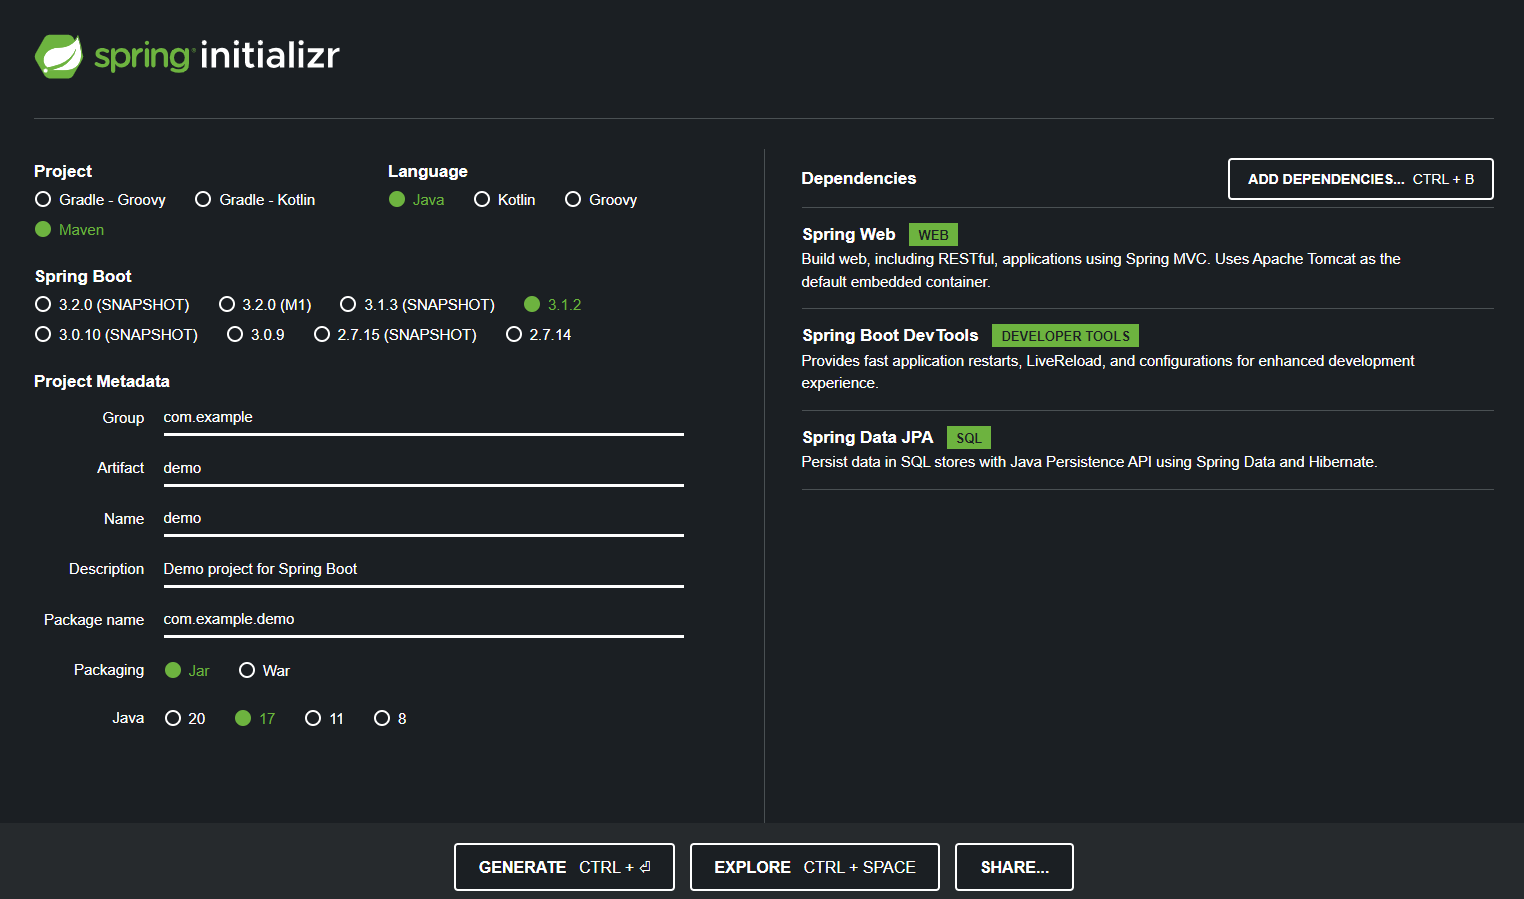
\includegraphics[width=0.95\columnwidth]{Spring_initializr} 
    \caption{Interfaccia Spring Initializr}
\end{figure}

\noindent \href{https://start.spring.io/}{Spring Initializr} è uno strumento online fornito dalla community di Spring Framework, che consente di creare rapidamente un progetto Spring Boot personalizzato, con le dipendenze e le configurazioni preselezionate dall'utente. Questo strumento semplifica notevolmente il processo di inizializzazione di un progetto Spring Boot, permettendo agli sviluppatori di risparmiare tempo e concentrarsi sulla scrittura del codice.\\
L'utente può selezionare il tipo di progetto di cui ha bisogno, come ad esempio un progetto Maven o Gradle, e specificare il linguaggio e la versione di Spring Boot desiderati. Inoltre, può anche inserire i metadati del progetto, come il nome del progetto e il nome dei packages.\\
Una volta selezionate le opzioni desiderate, l'utente può scegliere le dipendenze per il progetto. Le dipendenze sono librerie di terze parti che forniscono funzionalità aggiuntive al progetto.\\
Dopo aver selezionato le dipendenze, l'utente può scaricare il progetto Spring Boot personalizzato in formato ZIP. 

\subsection{Contenuto del pacchetto}
Il file ZIP scaricato precedentemente contiene tutti i file necessari per iniziare a lavorare sul progetto. All'interno di questo pacchetto troviamo i seguenti elementi rilevanti:
\begin{itemize}
\item file di configurazione \textit{application.properties} e file di build \textit{pom.xml} con le dipendenze selezionate;
\item classe principale, rappresenta il punto di ingresso dell'applicazione ed è annotata con \textit{@SpringBootApplication}. Il metodo \texttt{main()} al suo interno avvierà l'applicazione Spring;
\item una struttura base dei package.
\end{itemize}
\subsubsection{Pom.xml}
Di seguito riporto un frammento di codice del file di build \textit{pom.xml} che si ottiene creando un progetto con le dipendenze sopra selezionate. La configurazione di Maven avviene proprio tramite questo file.\\
All'interno di questo file si possono trovare i seguenti tag:
\begin{itemize}
\item \textit{<dependecies>}, indica una lista di dipendenze;
\item \textit{<build>}, contiene impostazioni di costruzione e compilazione;
\item \textit{<plugins>}, contiene plugin di Maven;
\item \textit{<properties>}, contiene proprietà definite dall'utente;
\item \textit{<groupId>}, organizzazione che ha creato il progetto;
\item \textit{<artifactId>}, nome unico del progetto;
\item \textit{<version>},  versione del progetto.
\end{itemize}

\noindent Nel file si possono notare le seguenti dipendenze:
\begin{itemize}
\item \textit{spring-boot-starter-web}, per utilizzare il framework Spring MVC per la creazione di applicazioni Web;
\item \textit{spring-boot-starter-jpa}, per la persistenza dei dati;
\item \textit{spring-boot-devtools}, offre tools per migliorare il processo di sviluppo;
\item \textit{spring-boot-starter-test}, per includere librerie di testing.
\end{itemize}

\begin{figure}[H] 
    \centering 
    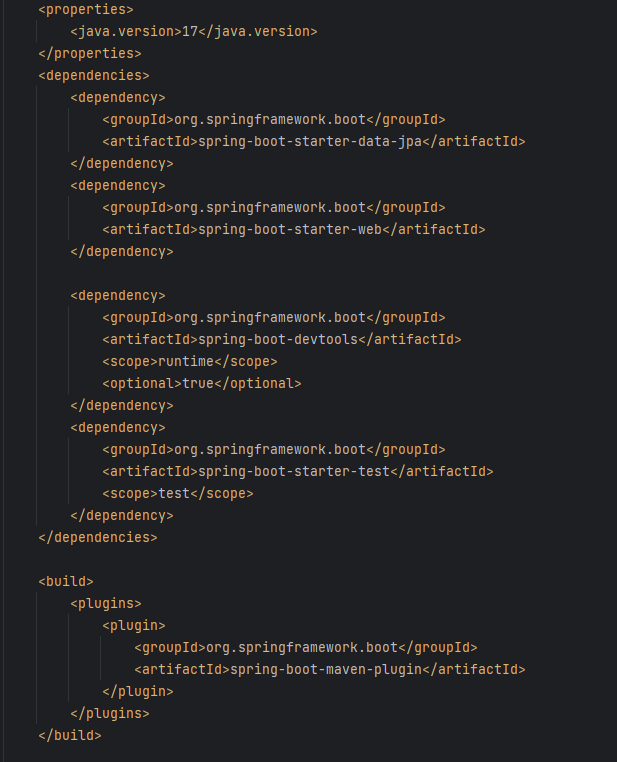
\includegraphics[width=0.70\columnwidth]{foto_pom_base} 
    \caption{Snippet pom.xml generato}
\end{figure}

Rispetto al file utilizzato nel progetto mancano le seguenti dipendenze:
\begin{itemize}
\item \textit{spring-boot-starter-jdbc}, per avviare Spring con il supporto JDBC nel progetto;
\item \textit{mssql-jdbc}, contenente il driver JDBC di Microsoft SQL Server;
\item \hypertarget{doc-api}{\textit{springdoc-openapi-starter-webmvc-ui}}, dipendenza per l'integrazione di Springdoc OpenAPI con Spring Boot per generare la documentazione dell'API utilizzando l'interfaccia utente WebMvc UI;
\item \textit{poi} e \textit{poi-ooxml}, due dipendenze relative ad Apache POI che offre funzionalità per poter lavorare con documenti Microsoft Office;
\item \textit{jxls-jexcel}, dipendenza che include la libreria jXLS per creare e manipolare documenti Excel;
\item \textit{fastexcel} e \textit{fastexcel-reader}, altre dipendenze inerenti a file Excel che offrono funzionalità per lettura,scrittura e modifica di questi file.
\end{itemize}
Per il testing sono state aggiunte:
\begin{itemize}
\item \textit{junit}, framework usato in Java per scrivere test unitari;
\item \textit{hamcrest-library}, libreria utile a scrivere asserzioni più espressive e comprensibili nei test unitari;
\item \textit{h2}, si tratta della dipendenza per la libreria H2 Database Engine, che è un database SQL. Utilizzato con scope "test" per crearne un'istanza temporanea e utilizzarlo nei test.
\end{itemize}

\subsubsection{Application.properties}
\noindent Il secondo file qui sotto rappresentato è il file configurazione \textit{application.properties}. Di seguito riporto il file che ho utilizzato nel progetto:
\begin{figure}[H] 
    \centering 
    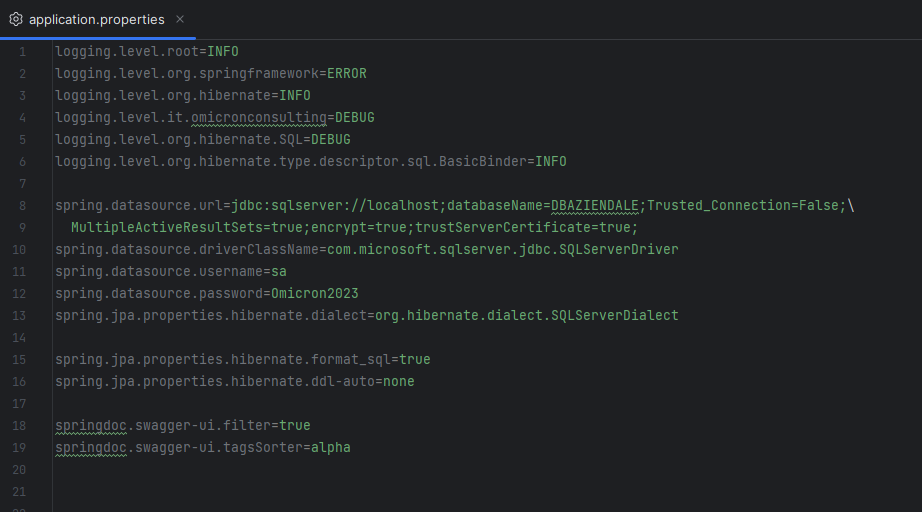
\includegraphics[width=0.85\columnwidth]{foto_application_properties} 
    \caption{Foto application.properties configurato e utilizzato}
\end{figure}

\noindent Possiamo notare come il file utilizzi un formato di configurazione basato su chiavi e valori. Le chiavi rappresentano le diverse proprietà di configurazione dell'applicazione, mentre i valori rappresentano le impostazioni specifiche.\\
Nel file possiamo notare le seguenti chaivi:
\begin{itemize}
\item \textit{logging.level}, servono per configurare il livello di dettaglio dei log per diverse classi o package all'interno dell'applicazione;
\item \textit{spring.datasource}, servono per collegarsi ad un database, in questo caso locale, inserendo username e password e driver di MSSQL;
\item \textit{spring.jpa.properties.hibernate}, serveono per configurare le impostazioni di Hibernate tra cui la validazione schema-entità, il dialetto\textsubscript{g} del server SQL e il suo livello di log;
\item \textit{springdoc.swagger-ui}, libreria che fornisce integrazione tra Spring Boot e Swagger UI.  
\end{itemize}. 









    \chapter{Modello dati}
\label{cap:database}
Questo capitolo descrive il database utilizzato all'interno del progetto.\\
Verrà descritto inizialmente la configurazione di Docker, passando per la struttura del database e la gestione dei log nel database.\\

\section{Configurazione di Docker}
I container Docker offrono un'isolamento completo dell'ambiente, che aiuta a evitare conflitti di dipendenze e interferenze con altre applicazioni o servizi che potrebbero essere presenti sul sistema. Per questo motivo si è deciso di utilizzare l'approccio di sandboxing\textsubscript{g} che offre Docker, poichè l'utilizzo di container consente di isolare le applicazioni e i servizi in ambienti virtualizzati, condividendo il kernel del sistema operativo host ma separando le loro risorse e i loro processi.\\
Dato che le tabelle di mia creazione dovevano integrarsi con il database aziendale, tramite il tool Docker Compose e un file di configurazione \textit{docker-compose.yaml}, è stato possibile avviare un nuovo container contenente un'immagine di Microsoft SQL Server, che forniva un backup del database aziendale con dati e tabelle.\\

\section{Progettazione del database}
\subsection{Configurazione di Docker}
I container Docker offrono un'isolamento completo dell'ambiente, che aiuta a evitare conflitti di dipendenze e interferenze con altre applicazioni o servizi che potrebbero essere presenti sul sistema. Per questo motivo si è deciso di utilizzare l'approccio di sandboxing\textsubscript{g} che offre Docker, poichè l'utilizzo di container consente di isolare le applicazioni e i servizi in ambienti virtualizzati, condividendo il kernel del sistema operativo host ma separando le loro risorse e i loro processi.\\
Dato che le tabelle di mia creazione dovevano integrarsi con il database aziendale, tramite il tool Docker Compose\textsubscript{g} e un file di configurazione \textit{docker-compose.yaml}, è stato possibile avviare un nuovo container contenente un'immagine di Microsoft SQL Server, che forniva un backup del database aziendale con dati e tabelle.\\

\subsection{Modello dati}
\textbf{IMMAGINE UML SENZA ATTRIBUTI}\\

\noindent Nel seguente disegno si può notare il database su cui poggia l'API.\\
È stata inserita una nomenclatura <<esterna>> per indicare le tabelle proveniente dal database aziendale.\\
Di seguito elenco le tabelle da me create, spiegandone l'utilizzo e gli attributi:\\

\noindent \textbf{TUTTE LE TABELLE MIE}\\



\section{Gestione dei log nel sistema}
Una tabella di log in un database è una struttura dati che registra le attività che si verificano su una tabella del database. I log sono utili per le seguenti finalità:
\begin{itemize}
\item Sicurezza, possono essere utilizzati per monitorare le attività e gli accessi nel database;
\item Risoluzione dei problemi, possono aiutare gli amministratori del database a capire la radice del problema, facilitando la risoluzione di bug;
\item Recupero dati, ritornano utili in caso di perdita di dati o di necessità a riprendere dati cancellati o modificati;
\end{itemize} 
Per soddisfare il requisito \hyperlink{rf64}{RFDE-64} è stata creata una tabella di log per le Pianificazioni.
Per limiti di tempo non è stata creata e gestita anche l'altra tabella di log delle Richieste come scritto nel requisito \hyperlink{rf46}{RFDE-46}.\\
\subsection{Tabella PianificazioniAudit}
La tabella di log per le Pianificazioni contiene tutti gli attributi di Pianificazioni, ma duplicati. Si distinguono in attributi "old", facendo riferimento ai valori della Pianificazione prima dell'operazione e "new", facendo riferimento ai valori della Pianificazione dopo l'operazione. La chiave primaria della tabella è una chiave composta da: Id della Pianificazione e timestamp dell'attività. Si possono notare anche gli attributi "Utente", per tenere traccia di chi ha effettuato la modifica e l'attributo "Operazione", per indicare se si tratta di un'operazione di cancellazione,inserimento o modifica.\\

\noindent Il popolamento di questa tabella avviene tramite un trigger\textsubscript{g} che si avvia non appena c'è un inserimento, un update o una delete di una riga nella tabella delle Pianificazioni.
\begin{figure}[H] 
    \centering 
    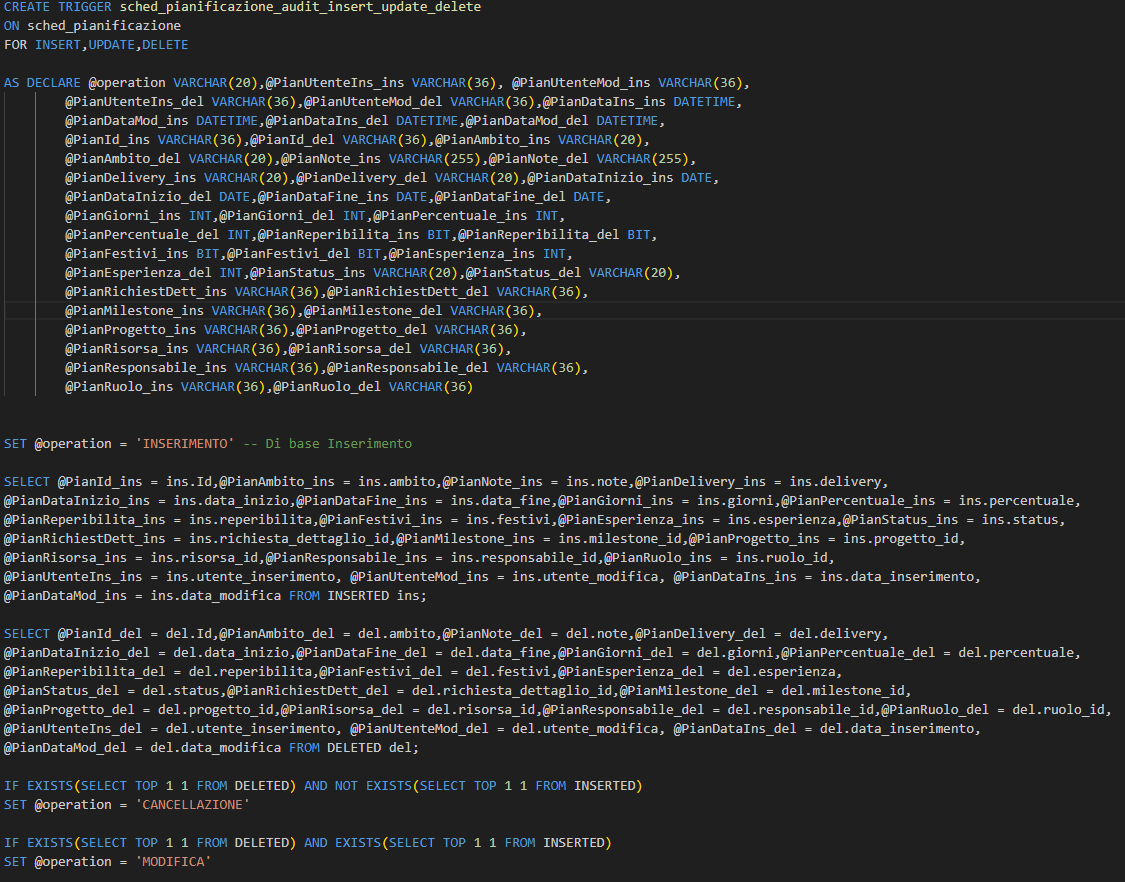
\includegraphics[width=1.0\columnwidth]{trigger-core} 
    \caption{Codice Trigger: Inizializzazione variabili}
\end{figure}

\begin{figure}[H] 
    \centering 
    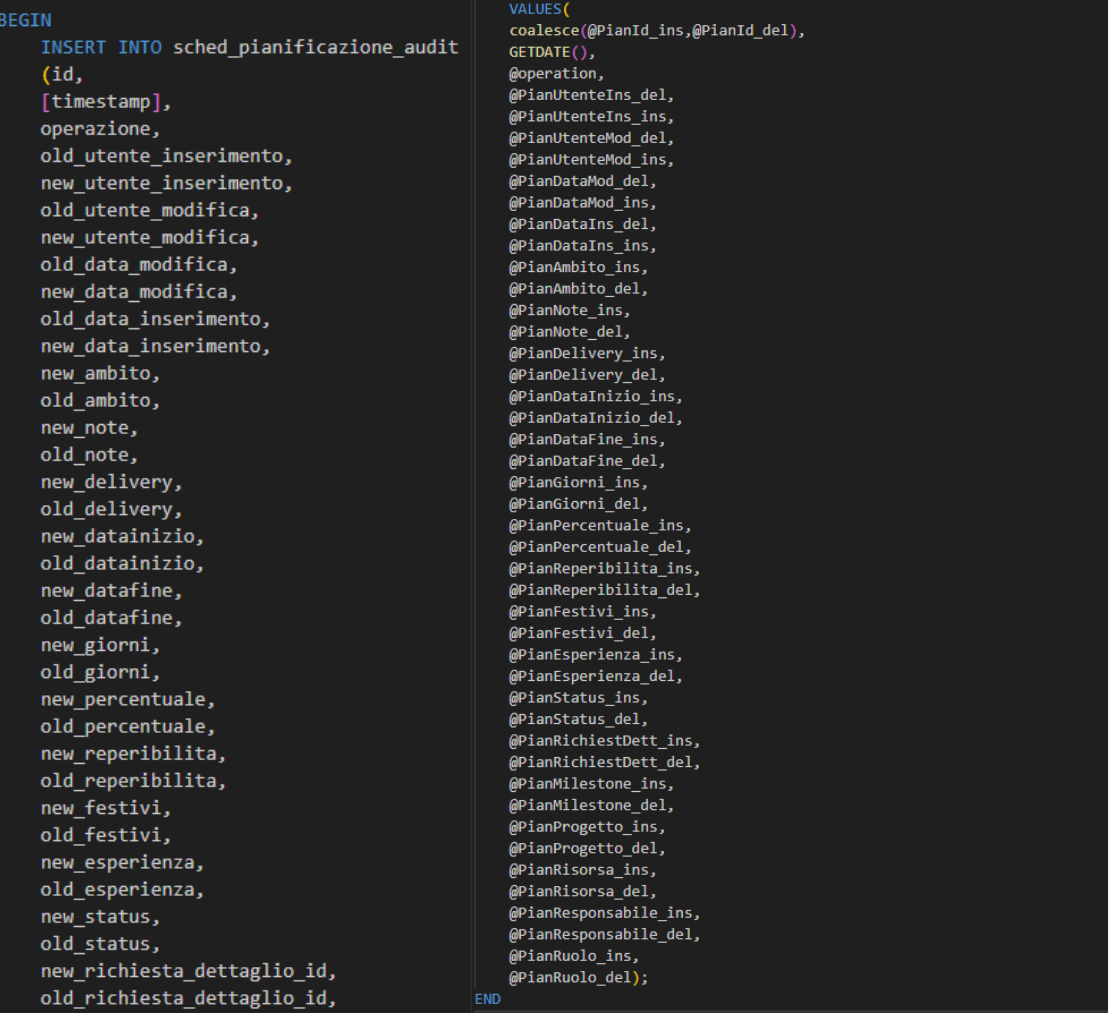
\includegraphics[width=0.8\columnwidth]{trigger-insert} 
    \caption{Codice Trigger: Inserimento dei valori nella tabella di log}
\end{figure}
\noindent Dopo aver definito le variabili, identificato l'operazione effettuata tramite un controllo, vengono eseguiti gli inserimenti nei campi appositi all'interno della tabella.



    \chapter{Sviluppo API REST}
\label{cap:api-rest}

Questo capitolo fornisce una spiegazione dettagliata dell'API che è stata sviluppata. Comprende informazioni sulle convenzioni di denominazione degli endpoint,i verbi HTTP utilizzati, una lista completa di tutti gli endpoint sviluppati e una descrizione del file Swagger che ha sostituito il mock iniziale dell'API.\\

\section{Convenzioni di denominazione REST}
Buona prassi nella creazione di un'API REST è il rispetto di convenzioni per la nomenclatura degli endpoint. Sebbene non esista un'unica convenzione obbligatoria, esistono delle best practices\textsubscript{g} per garantire una facile lettura e comprensibilità per agevolare gli sviluppatori che adoperano l'API.\\
Le seguenti convenzioni sono state rispettate nello sviluppo dell'API:
\begin{itemize}
\item  pluralizzare le risorse, per distinguere se si fa riferimento ad una lista di una determinata risorsa o ad una singola risorsa;
\item usare lettere minuscole;
\item non usare estensioni dei file;
\item in caso di nomi composti utilizzare il "-";
\item non usare underscore;
\item non utilizzare abbreviazioni o slang;
\item non utilizzare verbi, poichè l'azione dovrebbe essere indicata dal metodo HTTP utilizzato.
\end{itemize}

\section{Verbi standard HTTP}
I verbi standard forniti da HTTP utilizzati applicati all'API REST sono i seguenti:
\setlength{\arrayrulewidth}{0.3mm}
\renewcommand{\arraystretch}{2.5}
\begin{center}
\rowcolors{1}{white}{mygray}
\begin{longtable}{p{2cm}|p{8cm}}
\textbf{Verbo}  & \textbf{Descrizione}\\
\hline
%\rowcolor{mygray} 
POST   & Utilizzato per inviare dati al server al fine di creare una nuova risorsa ed aggiungerla all'insieme corrente\\
GET    & Utilizzato per richiedere dati al server in merito ad una o più risorse senza modificarle          \\
%\rowcolor{mygray}
DELETE &   Utilizzato per eliminare una risorsa specifica dal server          \\
PUT    &   Utilizzato per aggiornare totalmente una risorsa sovrascrivendola\\
%\rowcolor{mygray}
PATCH  &     Utilizzato per effettuare aggiornamenti parziali a una risorsa esistente        \\ 
\hline
\hiderowcolors
\caption{Verbi Standard HTTP utilizzati}
\label{tab:verbi-http}
\end{longtable}
\end{center}

%Per garantire una lettura chiara dello stato dell'operazione richiesta, sono stati utilizzati i seguenti codici di risposta HTTP. Questi codici 

\section{Endpoint sviluppati}
\noindent In questa sezione si trovano le descrizioni di tutti gli endpoint implementati, suddivisi in base all'ambito di interesse. Sarà fornito anche il verbo HTTP e il percorso necessario per effettuare ciascuna richiesta.\\
\subsection*{Anagrafiche}
Questi endpoint vengono utilizzati dal Program Manager per effettuare operazioni di lettura sulle anagrafiche aziendali. 
\setlength{\arrayrulewidth}{0.3mm}
\renewcommand{\arraystretch}{2.5}
\begin{center}
\rowcolors{1}{white}{mygray}
\begin{longtable}{p{1.3cm}|p{4.95cm}|p{5.7cm}}
\textbf{Verbo}  & \textbf{Path} & \textbf{Descrizione}\\
\hline
GET    & \texttt{/area-competenza/\{id\}} & Permette la lettura di un'Area di Compentenza dato l'ID\\
GET    & \texttt{/clienti} & Permette la lettura da DB di tutti i Clienti ottenendo come risposta la lista di tutti i Clienti\\
GET    & \texttt{/clienti/\{id\}} & Permette la lettura da DB di un Cliente dato l'Id ottenendo come risposta il Cliente corrispondente\\
GET    & \texttt{/risorse/\{id\}} & Permette la lettura da DB di un Risorsa dato l'Id ottenendo come risposta la Risorsa corrispondente\\
GET    & \texttt{/ruoli} & Permette la lettura da DB di tutti i Ruoli ottenendo come risposta la lista di tutti i Ruoli\\
GET    & \texttt{/ruoli/\{id\}} & Permette la lettura da DB di un Ruolo dato l'Id ottenendo come risposta il Ruolo corrispondente\\
GET    & \texttt{/skill} & Permette la lettura da DB di tutte le Skill ottenendo come risposta la lista di tutte le Skill\\
GET    & \texttt{/skill/\{id\}} & Permette la lettura da DB di una Skill dato l'Id ottenendo come risposta la Skill corrispondente\\
\hline
\hiderowcolors
\caption{Endpoint Anagrafiche sviluppati}
\label{tab:endpoint-anagrafiche-api}
\end{longtable}
\end{center}

\subsection*{Milestones}
Questi endpoint consentono la creazione, lettura, modifica ed eliminazione di Milestones. Vengono utilizzati principalmente dal Program Manager.
\setlength{\arrayrulewidth}{0.3mm}
\renewcommand{\arraystretch}{2.5}
\begin{center}
\rowcolors{1}{white}{mygray}
\begin{longtable}{p{1.3cm}|p{4.95cm}|p{5.7cm}}
\textbf{Verbo}  & \textbf{Path} & \textbf{Descrizione}\\
\hline
POST    & \texttt{/milestones} & Permette l'inserimento di una nuova Milestone, inserendo il Progetto associato, il Commerciale, la Pianificazione e altri dettagli.\\
POST    & \texttt{/milestones/list} & Rappresenta una POST di ricerca. Restituisce una lista di Milestone in base ai filtri inseriti dall'utente, alla parola chiave inserita nella quicksearch (q) e a un booleano che determina se applicare tutti i filtri in modo congiuntivo (AND) o disgiuntivo (OR).\\
PATCH    & \texttt{/milestones/\{id\}/type} & Permette la modifica del campo Type di una Milestone su DB.\\
GET    & \texttt{/milestones/\{id\}} & Permette la lettura da DB di una Milestone dato l'Id ottenendo come risposta la Milestone corrispondente.\\
DELETE    & \texttt{/milestones/\{id\}} & Permette l'eliminazione da DB di una Milestone dato l'Id ottenendo come risposta la Milestone eliminata.\\
\hline
\hiderowcolors
\caption{Endpoint Milestones sviluppati}
\label{tab:endpoint-milestones-api}
\end{longtable}
\end{center}

\subsection*{Pianificazioni}
Questi endpoint consentono la creazione, lettura, modifica ed eliminazione di Pianificazioni.
Vengono utilizzati principalmente dal Program Manager.
\setlength{\arrayrulewidth}{0.3mm}
\renewcommand{\arraystretch}{2.5}
\begin{center}
\rowcolors{1}{white}{mygray}
\begin{longtable}{p{1.3cm}|p{4.95cm}|p{5.7cm}}
\textbf{Verbo}  & \textbf{Path} & \textbf{Descrizione}\\
\hline
GET    & \texttt{/pianificazioni/\{id\}} & Permette la lettura da DB di una Pianificazione dato l'Id ottenendo come risposta la Pianificazione corrispondente.\\
PUT & \texttt{/pianificazioni/\{id\}} & Permette la modifica parziale o totale di campi di una Pianificazione su DB sovrascrivendola.\\
DELETE    & \texttt{/pianificazioni/\{id\}} & Permette l'eliminazione da DB di una Pianificazione dato l'Id ottenendo come risposta la Pianificazione eliminata.\\
POST    & \texttt{/pianificazioni} & Permette l'inserimento di una nuova Pianificazione ed eventuali entità associate come: risorsa, ruolo, milestone, progetto, responsabile e figura.\\
POST    & \texttt/{pianificazioni/xlsx} & Permette l'esportazione di report Excel di Pianificazioni in base a filtri inseriti dall'utente.\\
POST    & \texttt{/pianificazioni/list} & Rappresenta una POST di ricerca. Restituisce una lista di Pianificazioni in base ai filtri inseriti dall'utente, alla parola chiave inserita nella quicksearch (q) e a un booleano che determina se applicare tutti i filtri in modo congiuntivo (AND) o disgiuntivo (OR).\\
PATCH    & \texttt{/pianificazioni/\{id\}/times} & Permette la modifica dei campi Data Inizio e Data Fine di una Pianificazione su DB.\\
PATCH    & \texttt{/pianificazioni/\{id\}/festivi} & Permette la modifica del campo Festivi di una Pianificazione su DB.\\
GET    & \texttt{/pianificazioni/\{id\}/audit} & Permette la lettura delle modifiche effettuate su una Pianificazione dalla tabella di log.\\
\hline
\hiderowcolors
\caption{Endpoint Pianificazioni sviluppati}
\label{tab:endpoint-pianificazioni-api}
\end{longtable}
\end{center}


\subsection*{Richieste}
Questi endpoint consentono la creazione, lettura, modifica ed eliminazione di Richieste di Pianificazioni. Vengono utilizzati principalmente dal Project Manager.
\setlength{\arrayrulewidth}{0.3mm}
\renewcommand{\arraystretch}{2.5}
\begin{center}
\rowcolors{1}{white}{mygray}
\begin{longtable}{p{1.3cm}|p{4.95cm}|p{5.7cm}}
\textbf{Verbo}  & \textbf{Path} & \textbf{Descrizione}\\
\hline
GET    & \texttt{/richieste/\{id\}} & Permette la lettura da DB di una Richiesta dato l'Id ottenendo come risposta la Richiesta corrispondente.\\
PUT    & \texttt{/richieste/\{id\}} & Permette la modifica parziale o totale di campi di una Richiesta su DB sovrascrivendola.\\
DELETE    & \texttt{/richieste/\{id\}} & Permette l'eliminazione da DB di una Richiesta dato l'Id ottenendo come risposta la Richiesta eliminata.\\
POST    & \texttt{/richieste} & Permette l'inserimento di una nuova Richiesta, inserendo le Figure Professionali e le Skill richieste e altri dettagli.\\
POST    & \texttt{/richieste/list} & Rappresenta una POST di ricerca. Restituisce una lista di Richieste in base ai filtri inseriti dall'utente, alla parola chiave inserita nella quicksearch (q) e a un booleano che determina se applicare tutti i filtri in modo congiuntivo (AND) o disgiuntivo (OR).\\
DELETE    & \texttt{/richieste/\{id\}/stato} & Permette la modifica del campo Stato di una Richiesta su DB.\\
DELETE    & \texttt{/richieste/\{id\}/priorita} & Permette la modifica del campo Priorità di una Richiesta su DB.\\
\hline
\hiderowcolors
\caption{Endpoint Richieste sviluppati}
\label{tab:endpoint-richieste-api}
\end{longtable}
\end{center}


\section{Swagger}
%Spiegazione come è stata creata la grafica per gli endpoint con screen di un'interfaccia Controller.

Swagger è un framework utilizzato per la documentazione, progettazione e gestione di API REST.
Per garantire ordine sul mio lavoro e una comunicazione più trasparente e chiara con chi lavora nel lato Front-End è stato creato questo documento utilizzando lo standard OpenAPI.\\
Questo disegno dell'API ha sostituito poi il mock iniziale dell'API, considerando questo nuovo documento come unico per la consultazione dell'API finale.
\begin{figure}[H] 
    \centering 
    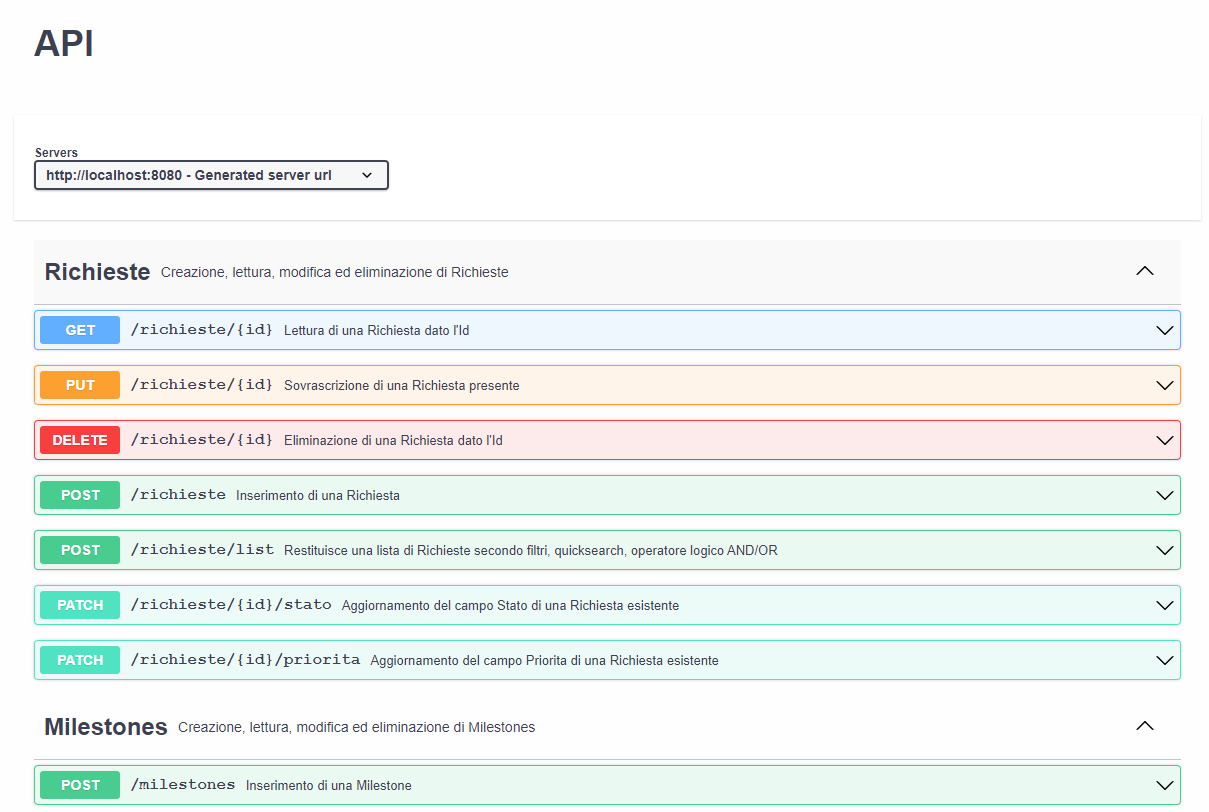
\includegraphics[width=0.95\columnwidth]{foto-swagger-titolo} 
    \caption{Inizio del documento di definizione dell'API}
\end{figure}
\noindent Il documento rappresenta un disegno completo dell'implementazione dell'API REST. Contiene tutti gli endpoint sviluppati, come sono strutturati al loro interno e arrichito di descrizioni per endpoint, risposte, richieste ed errori.
\begin{figure}[H] 
    \centering 
    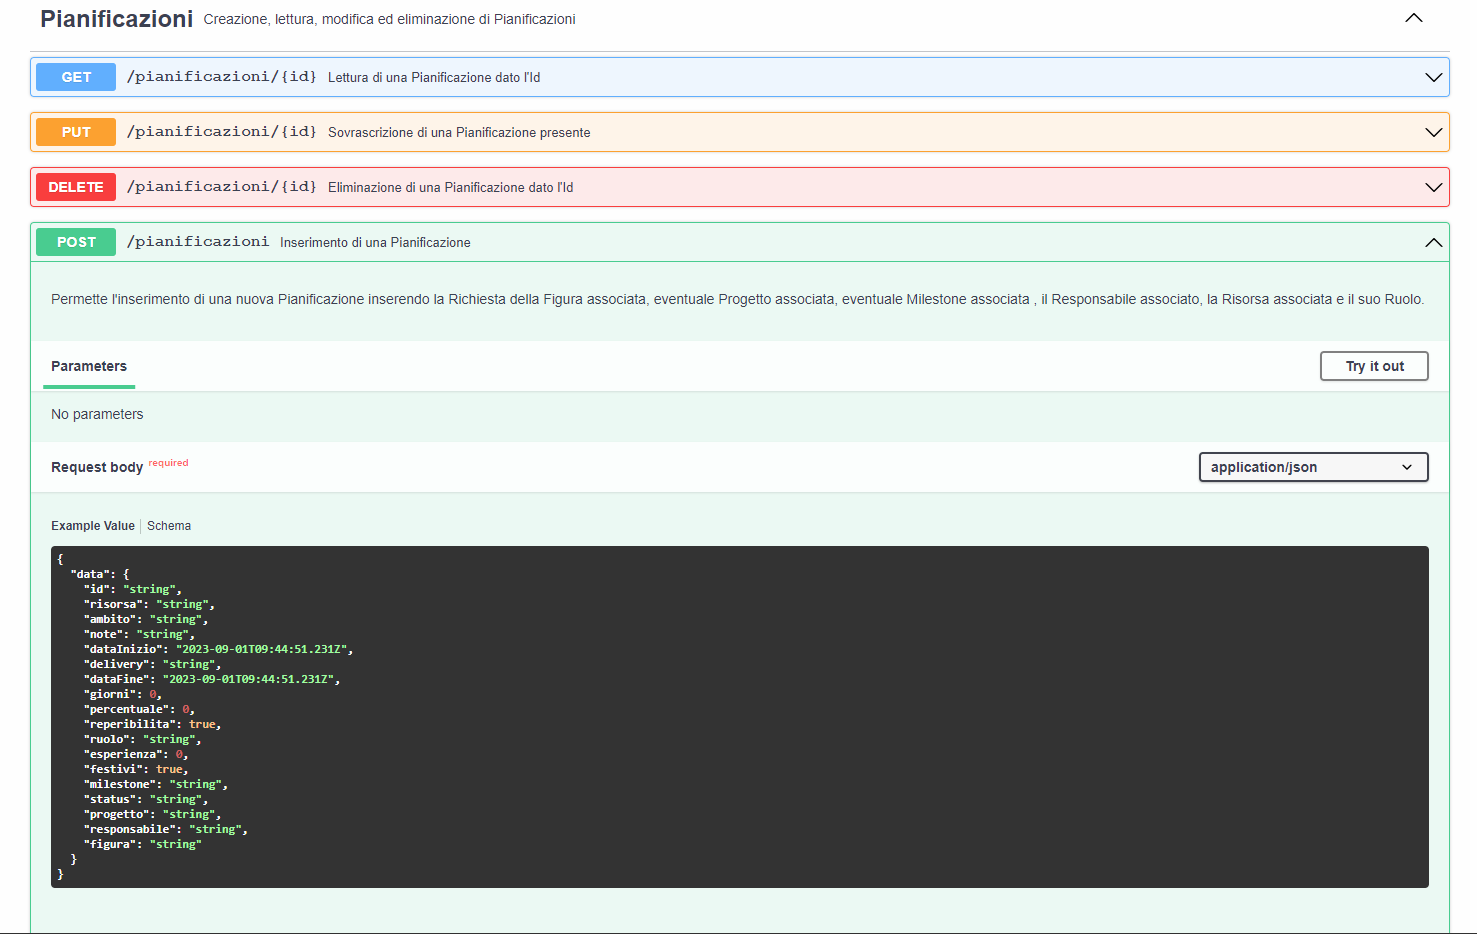
\includegraphics[width=0.95\columnwidth]{foto-swagger-example-value-2} 
    \caption{Example value del body richiesto dall'endpoint}
\end{figure}
\noindent In questa immagine possiamo notare un "Example value" del body richiesto da parte dell'endpoint POST /pianificazioni.\\
\begin{figure}[H] 
    \centering 
    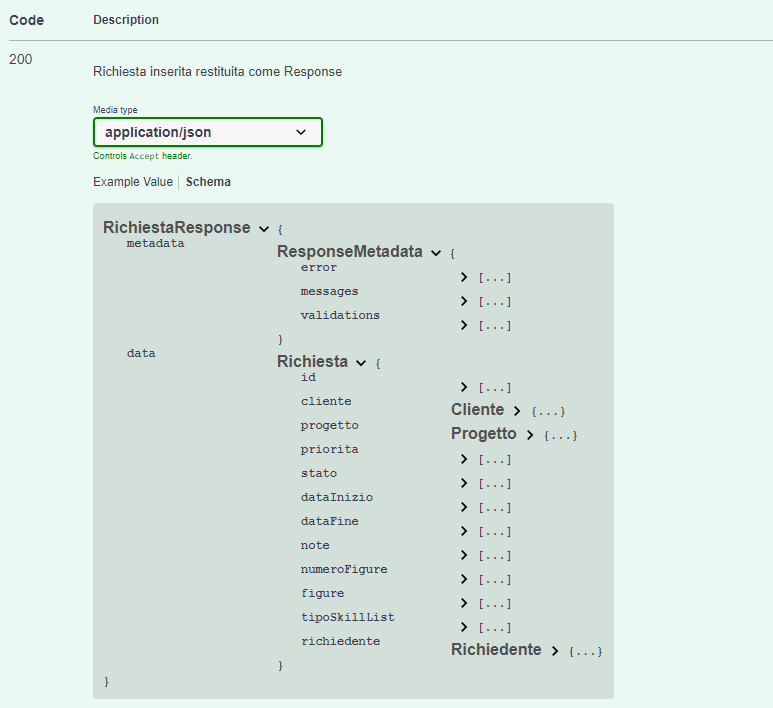
\includegraphics[width=0.65\columnwidth]{foto-swagger-composizione-oggetto} 
    \caption{Composizione oggetto response ritornato dall'endpoint}
\end{figure}
\noindent Inoltre, è possibile esaminare la struttura di ciascun oggetto, sia nelle richieste che nelle risposte. Questo è particolarmente vantaggioso per gli sviluppatori Front-End, poiché consente loro di interagire in modo accurato con il Back-End. In questo modo, il Back-End indica al Front-End cosa e come ci si aspetta di ricevere per quanto riguarda i dati nelle richieste, mentre il Front-End viene informato su come e cosa riceverà dal Back-End nelle risposte.
\begin{figure}[H] 
    \centering 
    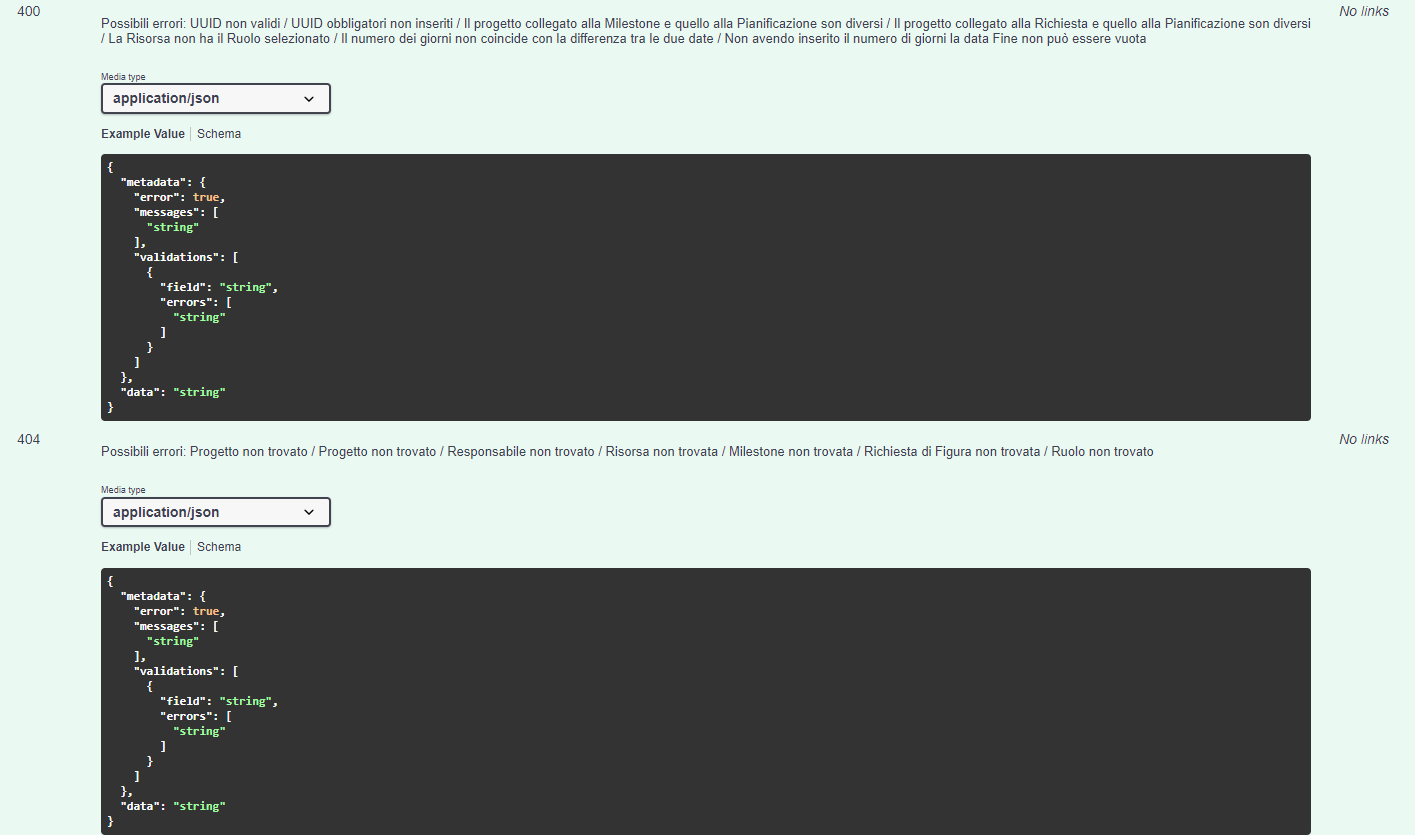
\includegraphics[width=1.00\columnwidth]{foto-swagger-errori} 
    \caption{Errori possibili in un endpoint}
\end{figure}
\noindent Per garantire una comprensione chiara dei possibili errori che potrebbero verificarsi, vengono identificate e descritte varie situazioni, ciascuna associata a un codice di errore specifico, al fine di fornire una struttura generale per codice di errore.

    \chapter{Codifica}
\label{cap:codifica}

\section{Scopo del capitolo}
Nel seguente capitolo si può osservare il lavoro dei giorni seguenti alla Progettazione fino agli ultimi giorni di tirocinio. In questo capitolo viene illustrato lo sviluppo dell'API REST, come è stato organizzato il codice parlando di classi e package, la codifica dei moduli più rilevanti ed infine la validazione. \\

\section{Convenzioni di denominazione REST}
Buona prassi nella creazione di un'API REST è il rispetto di convenzioni per la nomenclatura degli endpoint. Sebbene non esista un'unica convenzione obbligatoria, esistono delle best practices\textsubscript{g} per garantire una facile lettura e comprensibilità per agevolare gli sviluppatori che adoperano l'API.\\
Le seguenti convenzioni sono state rispettate nello sviluppo dell'API:
\begin{itemize}
\item  pluralizzare le risorse, per distinguere se si fa riferimento ad una lista di una determinata risorsa o ad una singola risorsa;
\item usare lettere minuscole;
\item non usare estensioni dei file;
\item in caso di nomi composti utilizzare il "-";
\item non usare underscore;
\item non utilizzare abbreviazioni o slang;
\item non utilizzare verbi, poichè l'azione dovrebbe essere indicata dal metodo HTTP utilizzato.
\end{itemize}

\section{Verbi standard HTTP}
I verbi standard forniti da HTTP utilizzati applicati all'API REST sono i seguenti:
\setlength{\arrayrulewidth}{0.3mm}
\renewcommand{\arraystretch}{2.5}
\begin{center}
\rowcolors{1}{white}{mygray}
\begin{longtable}{p{2cm}|p{8cm}}
\textbf{Verbo}  & \textbf{Descrizione}\\
\hline
%\rowcolor{mygray} 
POST   & Utilizzato per inviare dati al server al fine di creare una nuova risorsa ed aggiungerla all'insieme corrente\\
GET    & Utilizzato per richiedere dati al server in merito ad una o più risorse senza modificarle          \\
%\rowcolor{mygray}
DELETE &   Utilizzato per eliminare una risorsa specifica dal server          \\
PUT    &   Utilizzato per aggiornare totalmente una risorsa sovrascrivendola\\
%\rowcolor{mygray}
PATCH  &     Utilizzato per effettuare aggiornamenti parziali a una risorsa esistente        \\ 
\hline
\hiderowcolors
\caption{Verbi Standard HTTP utilizzati}
\label{tab:verbi-http}
\end{longtable}
\end{center}

%Per garantire una lettura chiara dello stato dell'operazione richiesta, sono stati utilizzati i seguenti codici di risposta HTTP. Questi codici 

\section{Endpoint sviluppati}
\noindent In questa sezione si trovano le descrizioni di tutti gli endpoint implementati, suddivisi in base all'ambito di interesse. Sarà fornito anche il verbo HTTP e il percorso necessario per effettuare ciascuna richiesta.\\
\subsection*{Anagrafiche}
Questi endpoint vengono utilizzati dal Program Manager per effettuare operazioni di lettura sulle anagrafiche aziendali. 
\setlength{\arrayrulewidth}{0.3mm}
\renewcommand{\arraystretch}{2.5}
\begin{center}
\rowcolors{1}{white}{mygray}
\begin{longtable}{p{1.3cm}|p{4.95cm}|p{5.7cm}}
\textbf{Verbo}  & \textbf{Path} & \textbf{Descrizione}\\
\hline
GET    & \texttt{/area-competenza/\{id\}} & Permette la lettura di un'Area di Compentenza dato l'ID\\
GET    & \texttt{/clienti} & Permette la lettura da DB di tutti i Clienti ottenendo come risposta la lista di tutti i Clienti\\
GET    & \texttt{/clienti/\{id\}} & Permette la lettura da DB di un Cliente dato l'Id ottenendo come risposta il Cliente corrispondente\\
GET    & \texttt{/risorse/\{id\}} & Permette la lettura da DB di un Risorsa dato l'Id ottenendo come risposta la Risorsa corrispondente\\
GET    & \texttt{/ruoli} & Permette la lettura da DB di tutti i Ruoli ottenendo come risposta la lista di tutti i Ruoli\\
GET    & \texttt{/ruoli/\{id\}} & Permette la lettura da DB di un Ruolo dato l'Id ottenendo come risposta il Ruolo corrispondente\\
GET    & \texttt{/skill} & Permette la lettura da DB di tutte le Skill ottenendo come risposta la lista di tutte le Skill\\
GET    & \texttt{/skill/\{id\}} & Permette la lettura da DB di una Skill dato l'Id ottenendo come risposta la Skill corrispondente\\
\hline
\hiderowcolors
\caption{Endpoint Anagrafiche sviluppati}
\label{tab:endpoint-anagrafiche-api}
\end{longtable}
\end{center}

\subsection*{Milestones}
Questi endpoint consentono la creazione, lettura, modifica ed eliminazione di Milestones. Vengono utilizzati principalmente dal Program Manager.
\setlength{\arrayrulewidth}{0.3mm}
\renewcommand{\arraystretch}{2.5}
\begin{center}
\rowcolors{1}{white}{mygray}
\begin{longtable}{p{1.3cm}|p{4.95cm}|p{5.7cm}}
\textbf{Verbo}  & \textbf{Path} & \textbf{Descrizione}\\
\hline
POST    & \texttt{/milestones} & Permette l'inserimento di una nuova Milestone, inserendo il Progetto associato, il Commerciale, la Pianificazione e altri dettagli.\\
POST    & \texttt{/milestones/list} & Rappresenta una POST di ricerca. Restituisce una lista di Milestone in base ai filtri inseriti dall'utente, alla parola chiave inserita nella quicksearch (q) e a un booleano che determina se applicare tutti i filtri in modo congiuntivo (AND) o disgiuntivo (OR).\\
PATCH    & \texttt{/milestones/\{id\}/type} & Permette la modifica del campo Type di una Milestone su DB.\\
GET    & \texttt{/milestones/\{id\}} & Permette la lettura da DB di una Milestone dato l'Id ottenendo come risposta la Milestone corrispondente.\\
DELETE    & \texttt{/milestones/\{id\}} & Permette l'eliminazione da DB di una Milestone dato l'Id ottenendo come risposta la Milestone eliminata.\\
\hline
\hiderowcolors
\caption{Endpoint Milestones sviluppati}
\label{tab:endpoint-milestones-api}
\end{longtable}
\end{center}

\subsection*{Pianificazioni}
Questi endpoint consentono la creazione, lettura, modifica ed eliminazione di Pianificazioni.
Vengono utilizzati principalmente dal Program Manager.
\setlength{\arrayrulewidth}{0.3mm}
\renewcommand{\arraystretch}{2.5}
\begin{center}
\rowcolors{1}{white}{mygray}
\begin{longtable}{p{1.3cm}|p{4.95cm}|p{5.7cm}}
\textbf{Verbo}  & \textbf{Path} & \textbf{Descrizione}\\
\hline
GET    & \texttt{/pianificazioni/\{id\}} & Permette la lettura da DB di una Pianificazione dato l'Id ottenendo come risposta la Pianificazione corrispondente.\\
PUT & \texttt{/pianificazioni/\{id\}} & Permette la modifica parziale o totale di campi di una Pianificazione su DB sovrascrivendola.\\
DELETE    & \texttt{/pianificazioni/\{id\}} & Permette l'eliminazione da DB di una Pianificazione dato l'Id ottenendo come risposta la Pianificazione eliminata.\\
POST    & \texttt{/pianificazioni} & Permette l'inserimento di una nuova Pianificazione ed eventuali entità associate come: risorsa, ruolo, milestone, progetto, responsabile e figura.\\
POST    & \texttt/{pianificazioni/xlsx} & Permette l'esportazione di report Excel di Pianificazioni in base a filtri inseriti dall'utente.\\
POST    & \texttt{/pianificazioni/list} & Rappresenta una POST di ricerca. Restituisce una lista di Pianificazioni in base ai filtri inseriti dall'utente, alla parola chiave inserita nella quicksearch (q) e a un booleano che determina se applicare tutti i filtri in modo congiuntivo (AND) o disgiuntivo (OR).\\
PATCH    & \texttt{/pianificazioni/\{id\}/times} & Permette la modifica dei campi Data Inizio e Data Fine di una Pianificazione su DB.\\
PATCH    & \texttt{/pianificazioni/\{id\}/festivi} & Permette la modifica del campo Festivi di una Pianificazione su DB.\\
GET    & \texttt{/pianificazioni/\{id\}/audit} & Permette la lettura delle modifiche effettuate su una Pianificazione dalla tabella di log.\\
\hline
\hiderowcolors
\caption{Endpoint Pianificazioni sviluppati}
\label{tab:endpoint-pianificazioni-api}
\end{longtable}
\end{center}


\subsection*{Richieste}
Questi endpoint consentono la creazione, lettura, modifica ed eliminazione di Richieste di Pianificazioni. Vengono utilizzati principalmente dal Project Manager.
\setlength{\arrayrulewidth}{0.3mm}
\renewcommand{\arraystretch}{2.5}
\begin{center}
\rowcolors{1}{white}{mygray}
\begin{longtable}{p{1.3cm}|p{4.95cm}|p{5.7cm}}
\textbf{Verbo}  & \textbf{Path} & \textbf{Descrizione}\\
\hline
GET    & \texttt{/richieste/\{id\}} & Permette la lettura da DB di una Richiesta dato l'Id ottenendo come risposta la Richiesta corrispondente.\\
PUT    & \texttt{/richieste/\{id\}} & Permette la modifica parziale o totale di campi di una Richiesta su DB sovrascrivendola.\\
DELETE    & \texttt{/richieste/\{id\}} & Permette l'eliminazione da DB di una Richiesta dato l'Id ottenendo come risposta la Richiesta eliminata.\\
POST    & \texttt{/richieste} & Permette l'inserimento di una nuova Richiesta, inserendo le Figure Professionali e le Skill richieste e altri dettagli.\\
POST    & \texttt{/richieste/list} & Rappresenta una POST di ricerca. Restituisce una lista di Richieste in base ai filtri inseriti dall'utente, alla parola chiave inserita nella quicksearch (q) e a un booleano che determina se applicare tutti i filtri in modo congiuntivo (AND) o disgiuntivo (OR).\\
DELETE    & \texttt{/richieste/\{id\}/stato} & Permette la modifica del campo Stato di una Richiesta su DB.\\
DELETE    & \texttt{/richieste/\{id\}/priorita} & Permette la modifica del campo Priorità di una Richiesta su DB.\\
\hline
\hiderowcolors
\caption{Endpoint Richieste sviluppati}
\label{tab:endpoint-richieste-api}
\end{longtable}
\end{center}


\subsubsection*{Common}
\begin{itemize}
\item \texttt{OmiPlanException}, eccezione custom utilizzata per gestire le \textit{RuntimeException}\textsubscript{g}. Classe formata da un HttpStatus per mostrare lo stato di risposta HTTP e dal messaggio fornito al lancio dell'eccezione;
\item \texttt{PaginationDirection}, classe enum per gestire la direzione della paginazione (ASC o DESC);
\item \texttt{SortDirectionVerifierConverter}, classe che implementa l'interfaccia \textit{Converter<S,T>} (componente Java utilizzato quando si lavora con strutture dati o oggetti che devono essere trasformati o adattatati in tipi diversi) per verificare che la direzione inserita sia ASC o DESC e gestire la \textit{RunTimeException} in caso non sia una variabile enum;
\item \texttt{StringToEnumConverter}, classe che implementa l'interfaccia \textit{Converter<S,T>} per convertire la direzione Stringa inserita nell'enum della direzione di pagina.
\end{itemize}

\subsubsection*{Config}
\begin{itemize}
\item \texttt{OmiPlanExceptionHandler}, handler\textsubscript{g} con il compito di gestire le eccezioni runtime e le altre segnandole come "Unexpected error". Questa classe è annotata con \textit{@ControllerAdvice}, poiché definisce una classe che gestisce in maniera centralizzata le eccezioni. Contiene due metodi annotati con \textit{@ExceptionHandler}che gestiscono rispettivamente le \textit{RunTimeException} e le altre eccezioni generali \textit{Exception};
\item \texttt{WebConfig}, classe annotata con l'annotazione \textit{@Configuration} indicando che è una classe di configurazione e che contiene definizioni di bean o altre configurazioni necessarie per l'applicazione. Essa infatti estende \textit{WebMvcConfigurer} che consente di modificare le configurazioni predefinite di Spring MVC, in questo caso aggiungendo i converter sopra citati.
\end{itemize}

\section{Package Entities}

\begin{figure}[H] 
    \centering 
    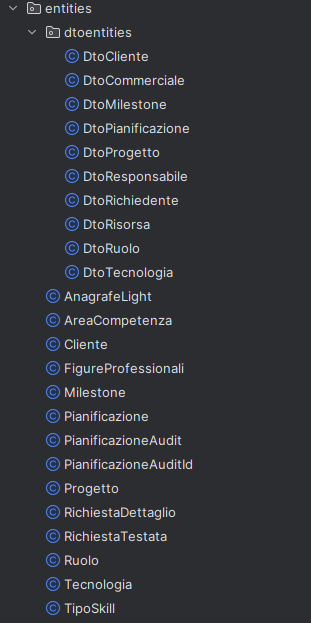
\includegraphics[width=0.4\columnwidth]{entities-package2} 
    \caption{Package entità}
\end{figure}

\noindent All'interno del package Entities troviamo le entità. Per entità si intendono tutte quelle classi Java che definiscono i modelli di dati dell'applicazione.\\
Queste classi vengono annotate con annotazioni JPA utili a stabilire come la classe venga associata a una tabella presente nel database relazionale. Ogni istanza di un'entità rappresenta una riga nella tabella relativa.\\
Di tutte le tabelle da me create è stata mappata ogni relazione tra tabelle e campo, mentre per ogni tabella del database aziendale sono stati mappati tutti i campi e le relazioni ad altre tabelle che potevano tornarmi utili.\\
In ogni entità troviamo setters e getters, costruttori con e senza argomenti.\\

\subsection{Esempio di un'entità}
\begin{figure}[H] 
    \centering 
    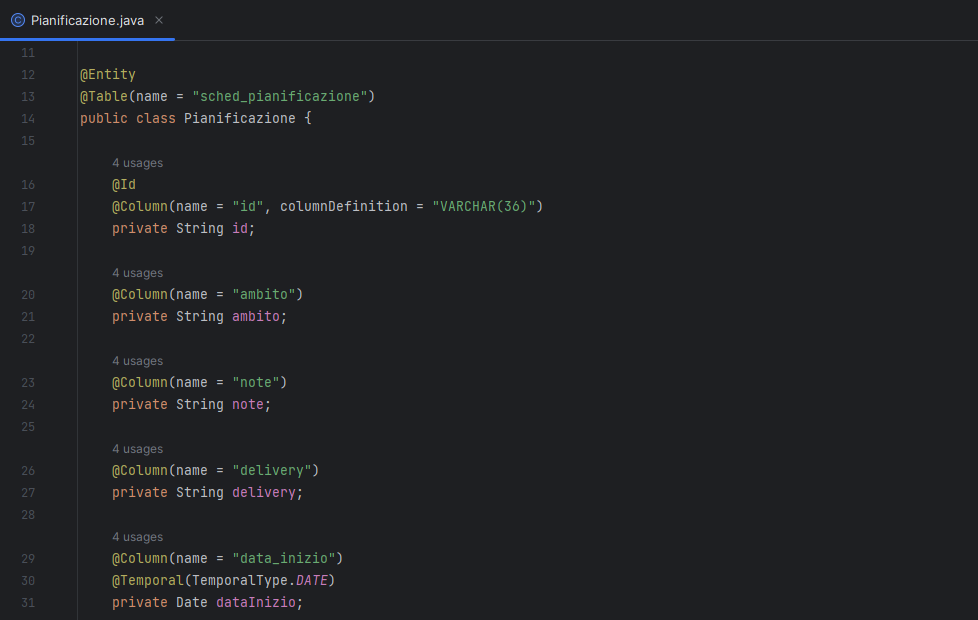
\includegraphics[width=0.9\columnwidth]{esempio-entita} 
    \caption{Esempio di mappatura di un'entità}
\end{figure}

\noindent Nell'immagine qui sopra possiamo notare uno snippet dell'entità Pianificazione in cui sono state utilizzate le seguenti annotazioni:
\begin{itemize}
\item \textit{@Entity}, per mappare le classi Java che rappresentano una tabella in un database si inserisce questa notazione specificando a class level\textsubscript{g}.
\item \textit{@Table}, nella maggior parte dei casi il nome di una tabella nel database e il nome dell'entità non sono gli stessi. Per questo motivo è stata utilizzata la seguente annotazione per specificare il nome della tabella;
\item \textit{@Column}, utilizzata per mappare una campo di una classe a una colonna di una tabella nel database. Questa annotazione possiede parametri come il "nome" per specificare il nome della colonna a cui è associato il campo;
\item \textit{@Id}, per identificare un campo all'interno di una classe come chiave primaria in una tabella del database viene utilizzata questa annotazione;
\item \textit{@Temporal}, utilizzata per specificare se un campo di tipo Date dovrebbe essere mappato come \textit{TemporalType.DATE}, per una data senza orario, \textit{TemporalType.TIME} per un orario senza data e infine \textit{TemporalType.TIMESTAMP}, utilizzato nella tabella di log di Pianificazione per mappare un campo con data e orario.
\end{itemize}
\subsection{Mappatura delle relazioni}
\begin{figure}[H] 
    \centering 
    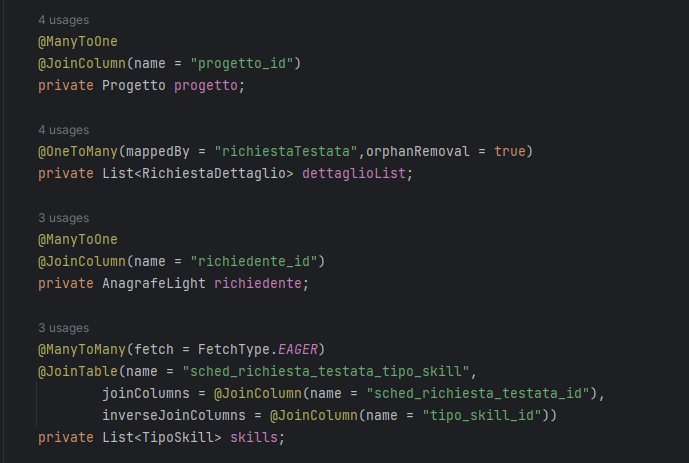
\includegraphics[width=0.9\columnwidth]{esempio-relazioni} 
    \caption{Esempio di mappatura delle relazioni della tabella RichiestaTestata}
\end{figure}
\noindent Per mantenere le relazioni tra le tabelle sono state utilizzate le annotazioni come nello snippet qui sopra raffigurante una porzione della classe Java che mappa la tabella RichiestaTestata.\\
In casi in cui entrambi i lati della relazione necessitavano per motivi implementativi, come la visualizzazione da entrambe le parti dell'informazione, di mappare la relazione opposta, veniva dichiarata una relazione bidirezionale, in cui entrambi i lati mappavano la relazione e diventava importante gestire correttamente la sincronizzazione tra le due entità.
\begin{itemize}
\item \textbf{uno-a-molti}, relazione in cui il campo associato sarà una lista di oggetti della classe opposta (in relazione all'esempio, una RichiestaTestata è associata a più RichiesteDettaglio), mentre nella relazione molti-a-uno sarà un oggetto singolo della classe opposta annotato con \textit{@JoinColumn} con \texttt{name} uguale a quello del campo nella tabella del database (in relazione all'esempio, una RichiestaTestata ha un solo Richiedente).\\
Nell'esempio è stato utilizzato il parametro \texttt{mappedBy} per mappare la relazione opposta e \texttt{orphanRemoval} per poter implementare la cancellazione di una RichiestaTestata garantendo l'eliminazione di tutte le RichiesteDettaglio associate al momento della rimozione.
\item \textbf{uno-a-uno}, relazione in cui un record della tabella è associato ad un solo record dell'altra tabella. Anche in questo caso se si vuole mappare da entrambi le parti la relazione bisogna utilizzare lo stesso principio dichiarato nella relazione \textit{@OneToMany}, solo che da entrambi le parti avranno come campo un oggetto della classe opposta.\\
Non sono state identificate relazioni uno-a-uno nel database.
\item \textbf{molti-a-molti}, relazione in cui viene mappata la tabella di join presente nel database tra le due tabelle, utilizzando il codice che si vede in esempio.
Per gestire operazioni di rimozione tra le due tabelle è stato utilizzato un metodo annotato con \textit{@PreRemove} nella classe TipoSkill, che entra in azione quando una RichiestaTestata viene eliminata, assicurando che la disconnessione avvenga in modo appropriato.
%\item \textbf{relazione bidirezionale}, relazione in cui è importante gestire correttamente la sincronizzazione tra le due direzioni della relazione, dato che quando si aggiorna una parte dell'entità bisogna aggiornare anche l'altra. Per mappare una relazione non è necessario mappare entrambi i lati della relazione, ma ritorna utile solo in base quello che si va ad implementare.
\end{itemize}
\subsection{Subpackage dtoentities}
All'interno del package "dtoentities" troviamo tutte quelle classi DTO delle entità di cui servivano soltanto determinate informazioni da restituire all'utente, evitando così ridondanza o informazioni superflue. Queste classi non contengono annotazioni, ma sono semplicemente degli oggetti contenenti i campi semplificati delle entità. A loro volta possono contenere altri DTO di altre entità in base alle relazioni che hanno.
\begin{figure}[H] 
    \centering 
    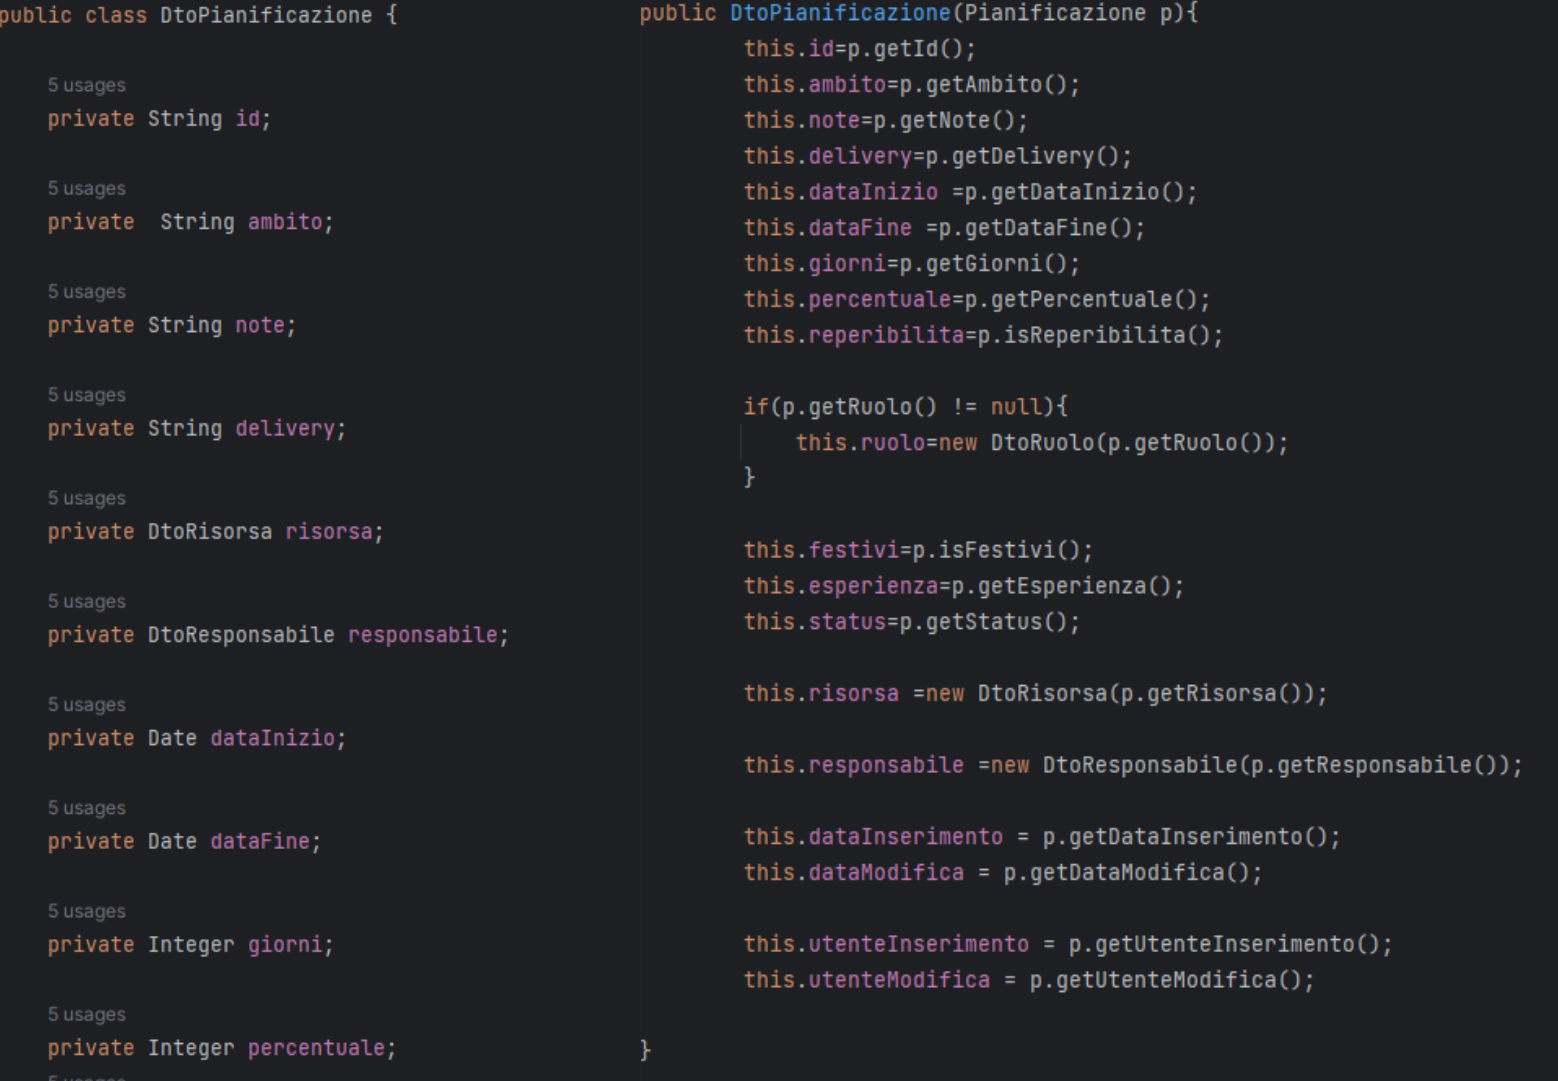
\includegraphics[width=0.9\columnwidth]{merge-dtopianificazione} 
    \caption{Esempio di classe DTO di Pianificazione}
\end{figure}
\noindent Ogni entità DTO possiede tre costruttori: costruttore senza argomenti e con argomenti e infine un costruttore che velocizzava la conversione da entità ad entità DTO (come mostrato nell'immagine qui sopra).

\section{Package dto}
Per la composizione delle richieste che il client invia o delle risposte che il server manda, sono state create vari tipi di requests e responses.\\
Ogni oggetto di risposta è composto da un oggetto "data" e un oggetto "metadata", mentre gli oggetti di richiesta possono variare. Se la richiesta è costruita per un endpoint che restituisce una lista di risultati, possiamo avere due casistiche:
\begin{itemize}
\item corpo della richiesta (body) formato da un oggetto "data", contenente informazioni utili alla risposta, e "metadata" che contiene i dati di paginazione;
\item nessun corpo, ma soltanto i dati di paginazione passati come parametri di query\textsubscript{g}.
\end{itemize}
Se invece la richiesta è costruita per un endpoint che restituisce un singolo oggetto nell'oggetto data, non viene utilizzato alcun body o parametri di query, ma solo una path variable.\\
Questa suddivisione "data" e "metadata" è un modello comune nella progettazione API per separare i dati effettivi o dati che forniscono informazioni per ottenere un tipo di risposta, dalle informazioni aggiuntive che descrivono il risultato o aggiungono caratteristiche alla richiesta.\\
Questo package è formato da vari subpackage.
\subsection{Common}
\begin{figure}[H] 
    \centering 
    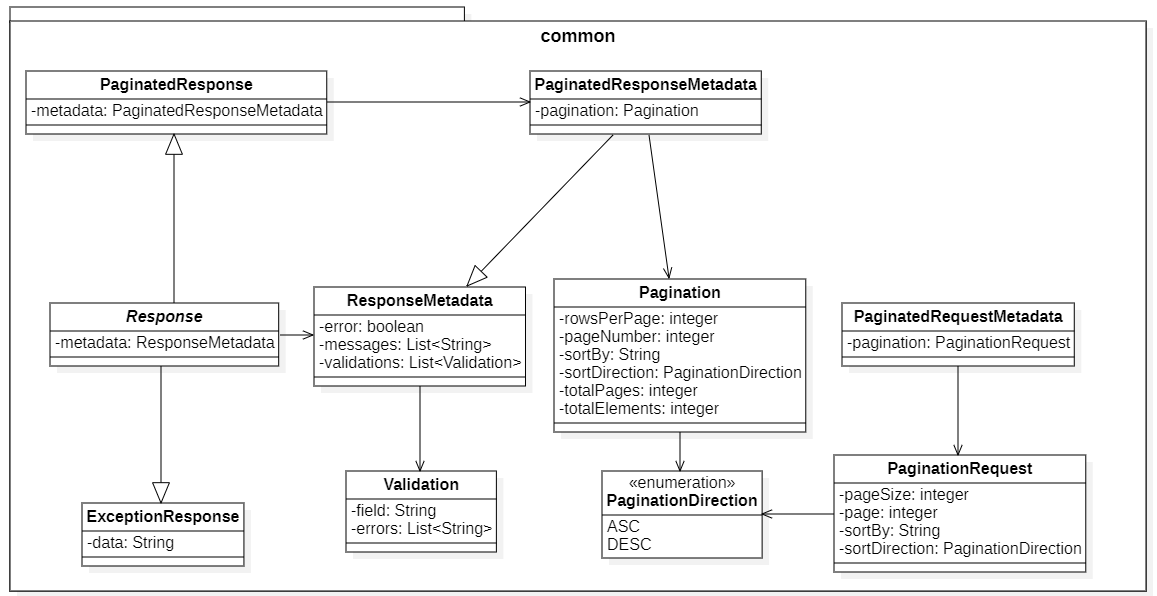
\includegraphics[width=1.0\columnwidth]{dto-sub-common} 
    \caption{Subpackage common}
\end{figure}
Questo subpackage contiene la response di base, response paginata, la response utilizzata nell'eccezione personalizzata, una request per la paginazione e i vari metadata utilizzati nelle responses.\\ Ogni \texttt{Metadata} contiene un boolean che indica se si è andati in errore (true) o meno (false), il messaggio di errore e una lista di \texttt{Validation}, contenente informazioni di validazione dei dati.\\
Ogni \texttt{Response} verrà poi estesa dalle classi che costituiscono le risposte ritornate per entità nel subpackage Responses.\\
È stata inoltre creata una classe \texttt{Pagination} per avere un controllo personalizzato sulla Paginazione.
\subsection{Requests e Body}
\begin{figure}[H] 
    \centering 
    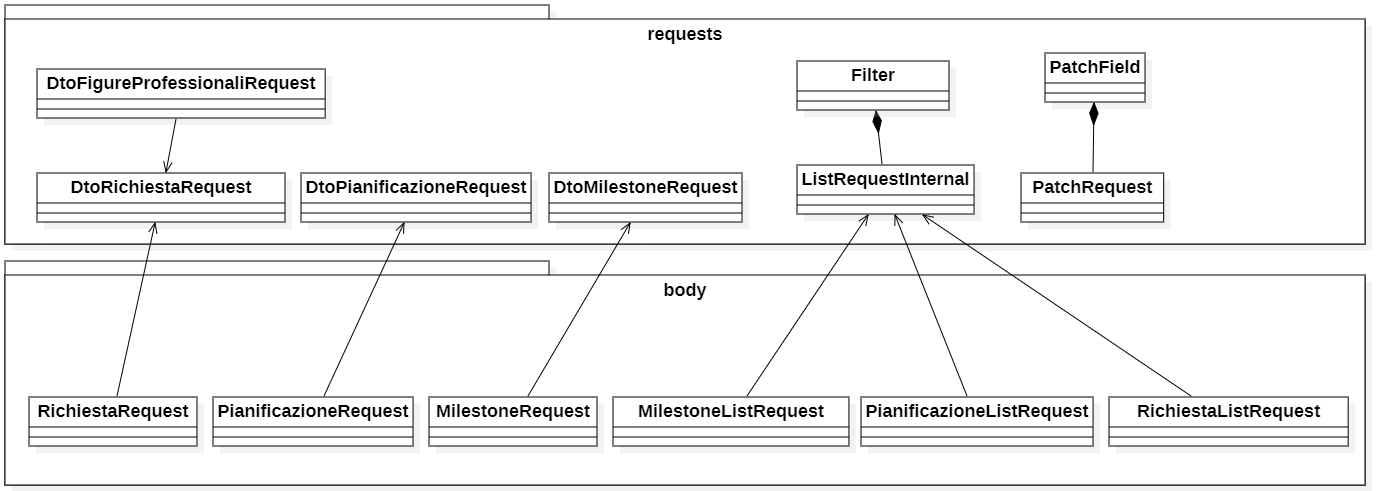
\includegraphics[width=1.0\columnwidth]{dto-sub-requests-body-2} 
    \caption{Subpackage requests e body}
\end{figure}
Questi due subpackages sono correlati tra di loro dato che ogni body ha come attributo una request presa dal subpackage requests.
Esistono due tipi di body:
\begin{itemize}
\item ogni \texttt{Request} singola è utilizzata per richiedere una specifica risorsa e contiene una request DTO formata dai campi utili che l'utente deve inserire;
\item ogni \texttt{ListRequest} è utilizzata per richiedere una o più risorse ed è formata da un oggetto data di tipo \texttt{ListRequestInternal}, che contiene tre parametri:
\begin{itemize}
\item filters, lista di oggetti \texttt{Filter} formati da campo-valore;
\item una stringa q (quicksearch) utile nella query personalizzata per cercare in determinati campi quello che l'utente inserisce;
\item andOperator per impostare i filtri in And o in Or nella query.
\end{itemize} 
\end{itemize}
All'interno del subpackage requests troviamo anche \texttt{PatchRequest}, contenente un unico campo corrispondente ad una lista di \texttt{PatchField}. Questa richiesta viene utilizzata nella richieste PATCH, in cui è possibile inserire uno o più valori in base a cosa si va a modificare.

\subsection{Responses}
\begin{figure}[H] 
    \centering 
    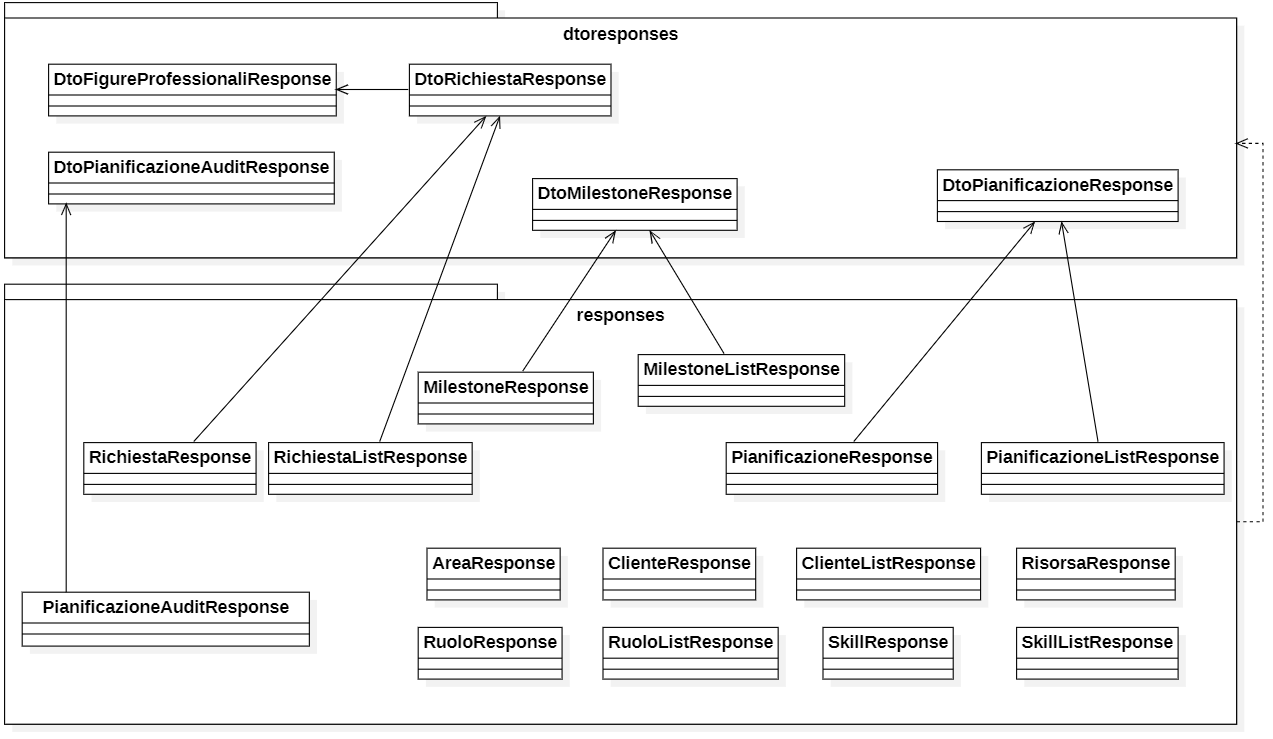
\includegraphics[width=0.9\columnwidth]{dto-sub-responses} 
    \caption{Subpackage responses e dtoresponses}
\end{figure}
Il package responses contiene tutte le response per entità. Ogni response estende la classe astratta \texttt{Response} se è una risposta singola, altrimenti estende la classe \texttt{PaginatedResponse} se è una lista di risposte. Questo permette all'utente di visualizzare la risposta, dopo aver interagito con un'endpoint, formata da "data" e "metadata".\\
Ogni response contiene un solo attributo che corrisponde all'oggetto "data" e può essere:
\begin{itemize}
\item una response DTO del subpackage dtoresponses;
\item un'entità DTO del subpackage delle entità;
\item in caso di una \texttt{ListResponse} l'attributo sarà una lista di response.
\end{itemize}

\subsection{Repository-Service-Controller}

\begin{figure}[H] 
    \centering 
    \includegraphics[width=0.85\columnwidth]{csp_img} 
    \caption{Schema di collegamento tra i componenti Repository,Service e Controller}
\end{figure}

\noindent Funzionamento.\\

\noindent \texttt{FOTO DI COME SONO NELLA DIRECTORY}\\

\noindent Presentazione di una Repository in particolare con spiegazione annotazioni.\\\\
Presentazione di una Service in particolare con spiegazione di un metodo in particolare, magari quello che excell che esegue la query.\\\\
Presentazione di un ControllerImpl in particolare con spiegazione annotazioni.\\\\

\subsection{Swagger UI}
Spiegazione come è stata creata la grafica per gli endpoint con screen di un'interfaccia Controller.



    \chapter{Verifica e Validazione}
\label{cap:verifica-validazione}

Questo capitolo descrive come è stata attuata la verifica e la validazione all'interno del progetto. Grazie al processo di verifica garantiamo che ogni attività dei processi svolti non introduca errori nel prodotto e che soddisfi i requisiti. Mentre con il processo di validazione viene determinato in maniera oggettiva che il prodotto sia conforme ai requisiti richiesti.\\
\section{Processo di verifica}
Durante tutto il periodo di tirocinio, ad ogni avanzamento di funzionalità e quindi cambio di requisito da soddisfare, con il tutor Antonio Fasolato è stato verificato che il codice sviluppato fino a quel momento fosse conforme con quanto aspettato e producesse output veritieri. Questo era aiutato inoltre dai controlli di validazione effettuati nei vari Controller e ulteriori controlli inseriti nei Service per garantire l’utilizzo di valori corretti.\\
Svolgendo le seguenti analisi regolarmente è stato possibile identificare e correggere errori evitando la loro propagazione nel corso della Codifica.
\subsection{Analisi statica}
Veniva effettuata un’analisi statica, che non richiede l'esecuzione del software, sul codice prodotto eseguendo prima un inspection, una lettura mirata e focalizzata sugli errori più noti e probabili, andando verso errori più specifici in base alla funzionalità implementata.
\subsection{Analisi dinamica}
L'analisi dinamica consiste nell'effettuare test sul prodotto in esecuzione. In caso di errore veniva eseguita un’ulteriore verifica successivamente alla mia correzione dell’errore che si era presentato.\\
\subsubsection{Debugging}
Per identificare al meglio un errore a run-time veniva usata la tecnica di debugging: consiste nell'individuazione e la correzione di errori che provocano anomalie rilevate durante l'esecuzione del programma. Questa tecnica è possibile grazie allo strumento di debugging che offre IntelliJ che permette di inserire dei breakpoint, cioè dei punti di interruzione nel codice, che non appena raggiunti durante l'esecuzione, sospende l'esecuzione ed è possibile ispezionare lo stato delle variabili, delle strutture dati e lo stack trace delle chiamate.\\ 
\subsubsection{Postman}
Per testare l'API veniva utilizzato il software Postman. Esso permetteva di osservare la response dell'endpoint in analisi per verificare che fosse conforme alle attese.\\

\begin{figure}[H] 
    \centering 
    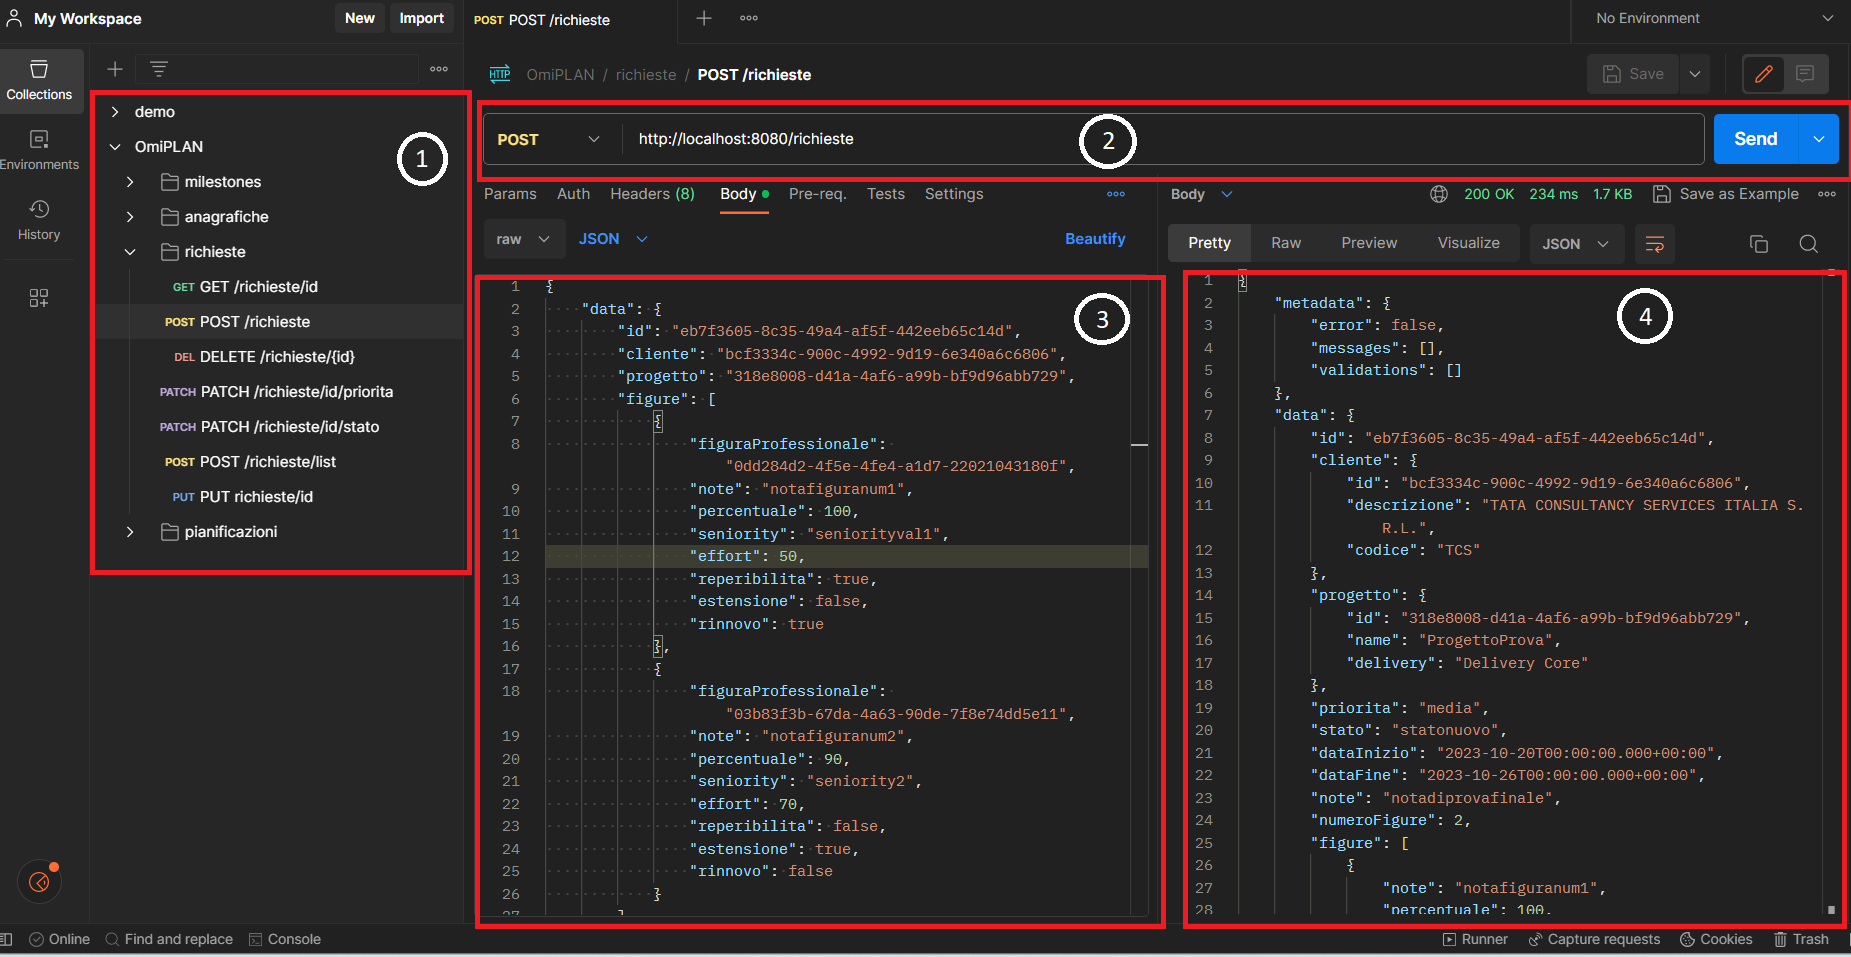
\includegraphics[width=0.95\columnwidth]{utilizzo-postman} 
    \caption{Interfaccia Postman}
\end{figure}
\noindent Per testare un endpoint si andava a configurare Postman nelle seguenti sezioni:
\begin{enumerate}
\item sezione in cui è possibile creare una nuova richiesta all'interno di una Collezione;
\item sezione in cui è possibile inserire l'URL che indica l'indirizzo del server e il percorso dell'endpoint a cui si desidera accedere, si seleziona il verbo HTTP e si aggiungono eventuali parametri di query. I parametri di query sono parte dell'URL che consente all'utente di filtrare, paginare o personalizzare i risultati;
\item sezione in cui è possibile inserire il body della request. Sopra al body si possono notare varie opzioni, di cui è stata utilizzata principalmente la sezione "Params", che permette di scrivere i parametri di query in modo più strutturato;
\item sezione in cui si potrà visualizzare la risposta in seguito al click sul pulsante "Send". La risposta sarà conforme alle specifiche selezionate.
\end{enumerate}

\hypertarget{testing}{\section{Testing}}
Per garantire la sicurezza e l’affidabilità, negli ultimi giorni di tirocinio, sono stati introdotti i test di unità.\\
Questo processo è iniziato con lo studio dei framework JUnit e Mockito.\\
I test di unità verificano il funzionamento corretto di singole unità di codice, come metodi o classi. Questi test vengono sviluppati isolandosi dalle dipendenze esterne permettendo di verificare che il codice funzioni correttamente e che produca risultati attesi.\\
È stato ritenuto ragionevole testare ciò che io avevo prodotto come metodi o classi. Componenti introdotti da librerie o framework non hanno necessitato di test, dando per assodato il loro funzionamento.\\
Dato il poco tempo rimanente, per mettere in pratica quanto appreso, si è deciso di limitare lo svolgimento dei test su un \textit{@Service} semplice, \texttt{MilestoneService}, andando a testare il corretto funzionamento dei suoi metodi.

\subsection{Esempio di un test effettuato}
\begin{figure}[H] 
    \centering 
    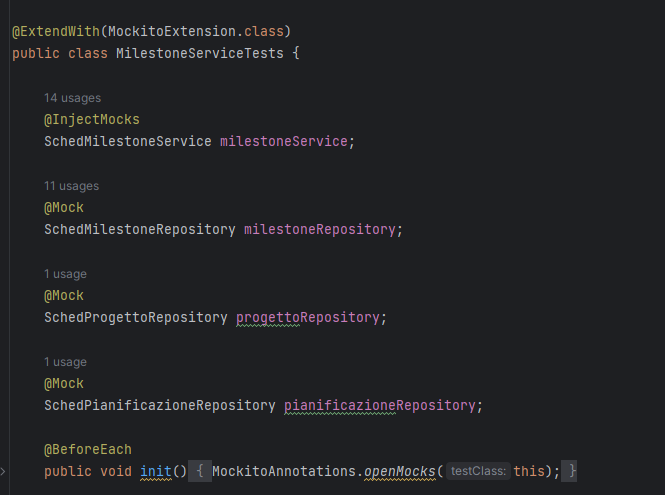
\includegraphics[width=0.85\columnwidth]{config-test} 
    \caption{Configurazione ambiente di testing}
\end{figure}
Per poter eseguire dei test su oggetti simulati (mock) è stata utilizzata l'annotazione \textit{@Mock} che ha permesso di creare i componenti mock da iniettare all’interno del Service sotto test, tramite l’annotazione \textit{@InjectMocks}. Tramite il metodo \texttt{init()}, annotato con \textit{@BeforeEach}, inizializziamo i componenti che vogliamo mockare permettendo l’utilizzo delle annotazioni che Mockito fornisce.\\
Qui sotto riporto un code snippet dei controlli eseguiti nel test relativo al metodo di creazione di una nuova Milestone. Per garantire il corretto funzionamento della creazione della Milestone, è stata testata ogni parte delicata che avrebbe compromesso il funzionamento del metodo, controllando l’eccezione sollevata, al momento dell’errore, assicurando che fosse quella corretta.\\

\begin{figure}[H] 
    \centering 
    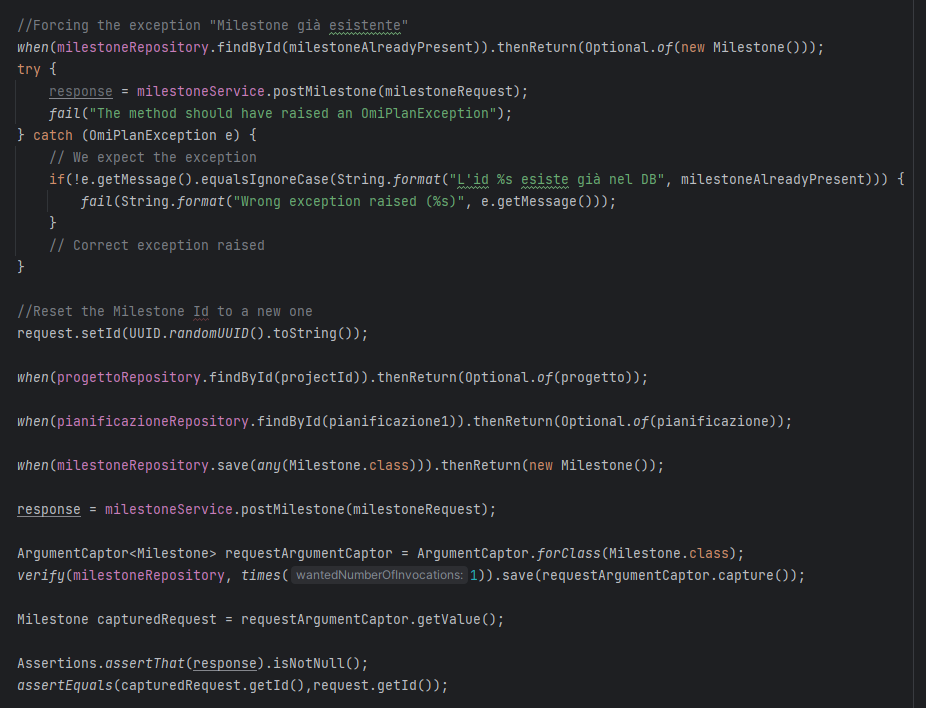
\includegraphics[width=0.9\columnwidth]{snippet-saveMilestone} 
    \caption{Code snippet test di creazione di una nuova Milestone}
\end{figure}

\noindent In questo snippet possiamo osservare come è stato forzato il lancio dell’eccezione quando si va a creare una Milestone con Id già esistente, controllando che sia stata proprio quella l’eccezione lanciata dal metodo.\\
Mockito offre strumenti, come il metodo \texttt{when()}, che consentono di effettuare stubbing\textsubscript{g} dei metodi, simulando il loro comportamento. Questo permette di definire come tali metodi dovrebbero rispondere quando vengono invocati, restituendo risultati specifici anziché eseguire il codice reale.\\ 
Un ulteriore metodo fornito da Mockito è \texttt{verify()}, utilizzato per controllare che il metodo \texttt{save()} della repository della Milestone venga chiamato una sola volta. Con \texttt{ArgumentCaptor<>} (che permette di raccogliere i parametri passati in una funzione) andiamo a "catturare" la Milestone salvata col metodo \texttt{save()}.\\
Per accertare che questa parte di test abbia avuto successo è stato verificato che la response ricevuta dal metodo non fosse vuota e, dato che il DTO restituito differisce per alcune caratteristiche dall’istanza completa di una Milestone, non è stato possibile un confronto intero tra i due oggetti, ed è stato ritenuto esaustivo garantire l’uguaglianza dei due Id. Queste verifiche sono state effettuate tramite metodi di asserzione forniti da JUnit.
Con l’ausilio di queste metodologie è stato possibile simulare e controllare la corretta creazione di una Milestone.\\

\section{Validazione}
Nell’ultimo giorno di tirocinio si è tenuto un incontro conclusivo insieme al tutor Antonio Fasolato e al \textit{RUOLO\_LAVORATIVO} Giovanni Incammicia, a conferma definitiva della conformità alle specifiche richieste del prodotto finale. Durante questa riunione, è stata effettuata una revisione dell'Analisi dei Requisiti fornita all'inizio del progetto, con particolare attenzione ai requisiti di mia competenza, al fine di verificare il loro soddisfacimento. Tuttavia, per scrivere il codice dell’API, è stato utilizzato principalmente un disegno iniziale dell’API e l’Analisi dei Requisiti fornita è stata utilizzata per aiutare la comprensione di alcuni endpoint. Questo approccio ha comportato alcune discrepanze tra le funzionalità implementate e i requisiti specificati. Rispetto all’Analisi dei Requisiti mancavano degli attributi che il Front-end necessitava o alcune funzionalità che necessitavano implementazioni particolari o di collegamenti a servizi esterni di cui non c’era tempo a sufficienza per poter studiare. Nonostante queste mancanze, analizzando le funzionalità implementate e le response fornite, è stato ritenuto sufficiente per il soddisfacimento dei requisiti di cui gli endpoint sviluppati facevano parte.\\
A causa delle problematiche da me sopra menzionate, non è stato possibile condurre una fase di Collaudo effettiva per valutare l'interazione tra il Front-end e il Back-end.
    \chapter{Deploy dell'applicazione}
\label{cap:deploy}
\section{Scopo del capitolo}
Al termine dell'attività di stage, insieme al tutor, ho potuto osservare come avviene il deploy di una Spring Boot app su Docker.\\
Per deployment del software si intende la distribuzione o avviamento, con relativa installazione e configurazione, di un'applicazione. È considerabile come fase finale del ciclo di vita di un software, fase che conclude lo sviluppo e il collaudo, dando inizio alla manutenzione.
\section{Deploy}
\subsection{Dockerfile}
Per cominciare è stato creato un \texttt{Dockerfile} nella root del progetto. Questo file definirà come Docker dovrebbe costruire l'immagine.
\begin{figure}[H] 
    \centering 
    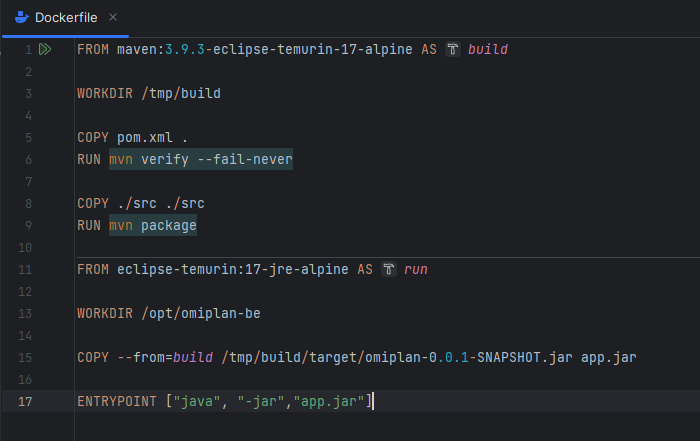
\includegraphics[width=0.80\columnwidth]{dockerfile} 
    \caption{Configurazione Dockerfile}
\end{figure}
\noindent All'interno del file, possiamo notare due sezioni separate, quella di build e quella di run (esecuzione).
\subsubsection*{Sezione Build}
Nella sezione di "build" viene indicato che si sta costruendo un'immagine di Docker basata su Maven 3.9.3 e Java 17. Vengono poi eseguite operazioni relative alla compilazione dell'applicazione, come la copia del file sorgente, la verifica delle dipendenze tramite il tool di build Maven e la crazione del pacchetto \texttt{.jar}.
\subsubsection*{Sezione Run}
La sezione di "run" ha come obiettivo l'esecuzione dell'applicazione. In questa sezione viene utilizzata nuovamente la stessa immagine di Java e vengono copiati i risultati della prima fase. L'istruzione finale \texttt{ENTRYPOINT} definisce il comando che verrà eseguito quando il container basato su questa immagine verrà avviato.
\subsection{Costruzione dell'immagine e avvio dell'applicazione}
In seguito alla creazione del \texttt{Dockerfile} si apre il terminale nella directory in cui si trova questo file.\\
Seguono poi i seguenti passi:
\begin{enumerate}
\item viene eseguito il comando \texttt{docker build -t nome\_immagine} per creare l'immagine Docker con le specifiche selezionate;
\item una volta costruita l'immagine si può avviare il container tramite il comando \texttt{docker run -ti nome\_immagine}; 
\item per accedere all'applicazione è possibile utilizzare un browser digitando il seguente indirizzo per interagire con l'applicazione: \textit{http://localhost:porta\_scelta}.
\end{enumerate}





%    \chapter{Analisi dei requisiti}
\label{cap:analisi-requisiti}

\intro{Breve introduzione al capitolo}\\

\section{Casi d'uso}

Per lo studio dei casi di utilizzo del prodotto sono stati creati dei diagrammi.
I diagrammi dei casi d'uso (in inglese \emph{Use Case Diagram}) sono diagrammi di tipo \gls{uml} dedicati alla descrizione delle funzioni o servizi offerti da un sistema, così come sono percepiti e utilizzati dagli attori che interagiscono col sistema stesso.
Essendo il progetto finalizzato alla creazione di un tool per l'automazione di un processo, le interazioni da parte dell'utilizzatore devono essere ovviamente ridotte allo stretto necessario. Per questo motivo i diagrammi d'uso risultano semplici e in numero ridotto.

\begin{figure}[!h] 
    \centering 
    \includegraphics[width=0.9\columnwidth]{usecase/scenario-principale} 
    \caption{Use Case - UC0: Scenario principale}
\end{figure}

\begin{usecase}{0}{Scenario principale}
\usecaseactors{Sviluppatore applicativi}
\usecasepre{Lo sviluppatore è entrato nel plug-in di simulazione all'interno dell'IDE}
\usecasedesc{La finestra di simulazione mette a disposizione i comandi per configurare, registrare o eseguire un test}
\usecasepost{Il sistema è pronto per permettere una nuova interazione}
\label{uc:scenario-principale}
\end{usecase}

\section{Tracciamento dei requisiti}

Da un'attenta analisi dei requisiti e degli use case effettuata sul progetto è stata stilata la tabella che traccia i requisiti in rapporto agli use case.\\
Sono stati individuati diversi tipi di requisiti e si è quindi fatto utilizzo di un codice identificativo per distinguerli.\\
Il codice dei requisiti è così strutturato R(F/Q/V)(N/D/O) dove:
\begin{enumerate}
	\item[R =] requisito
    \item[F =] funzionale
    \item[Q =] qualitativo
    \item[V =] di vincolo
    \item[N =] obbligatorio (necessario)
    \item[D =] desiderabile
    \item[Z =] opzionale
\end{enumerate}
Nelle tabelle \ref{tab:requisiti-funzionali}, \ref{tab:requisiti-qualitativi} e \ref{tab:requisiti-vincolo} sono riassunti i requisiti e il loro tracciamento con gli use case delineati in fase di analisi.

\newpage

\begin{table}%
\caption{Tabella del tracciamento dei requisti funzionali}
\label{tab:requisiti-funzionali}
\begin{tabularx}{\textwidth}{lXl}
\hline\hline
\textbf{Requisito} & \textbf{Descrizione} & \textbf{Use Case}\\
\hline
RFN-1     & L'interfaccia permette di configurare il tipo di sonde del test & UC1 \\
\hline
\end{tabularx}
\end{table}%

\begin{table}%
\caption{Tabella del tracciamento dei requisiti qualitativi}
\label{tab:requisiti-qualitativi}
\begin{tabularx}{\textwidth}{lXl}
\hline\hline
\textbf{Requisito} & \textbf{Descrizione} & \textbf{Use Case}\\
\hline
RQD-1    & Le prestazioni del simulatore hardware deve garantire la giusta esecuzione dei test e non la generazione di falsi negativi & - \\
\hline
\end{tabularx}
\end{table}%

\begin{table}%
\caption{Tabella del tracciamento dei requisiti di vincolo}
\label{tab:requisiti-vincolo}
\begin{tabularx}{\textwidth}{lXl}
\hline\hline
\textbf{Requisito} & \textbf{Descrizione} & \textbf{Use Case}\\
\hline
RVO-1    & La libreria per l'esecuzione dei test automatici deve essere riutilizzabile & - \\
\hline
\end{tabularx}
\end{table}%

%    \chapter{Progettazione e codifica}
\label{cap:progettazione-codifica}

\intro{Breve introduzione al capitolo}\\

\section{Tecnologie e strumenti}
\label{sec:tecnologie-strumenti}

Di seguito viene data una panoramica delle tecnologie e strumenti utilizzati.

\subsection*{Tecnologia 1}
Descrizione Tecnologia 1.

\subsection*{Tecnologia 2}
Descrizione Tecnologia 2

\section{Ciclo di vita del software}
\label{sec:ciclo-vita-software}

\section{Progettazione}
\label{sec:progettazione}

\subsubsection{Namespace 1} %**************************
Descrizione namespace 1.

\begin{namespacedesc}
    \classdesc{Classe 1}{Descrizione classe 1}
    \classdesc{Classe 2}{Descrizione classe 2}
\end{namespacedesc}


\section{Design Pattern utilizzati}

\section{Codifica}

%    \chapter{Verifica e validazione}
\label{cap:verifica-validazione}

    \chapter{Conclusioni}
\label{cap:conclusioni}

Il mio percorso è iniziato con lo studio dei concetti di base e delle tecnologie che avrei utilizzato, sotto la guida del tutor Antonio Fasolato, prima di passare alle esercitazioni sulle tecnologie.\\
Tra le esercitazioni iniziali, quella su SpringBoot è risultata essere la più complessa. Essendo concetti nuovi che andavo ad affrontare, come l'utilizzo delle annotazioni di SpringBoot, non è stato semplice all’inizio comprendere il funzionamento del framework e questo ha portato ad un maggior investimento di tempo rispetto alle altre esercitazioni. È stato comunque un investimento proficuo poichè ha permesso di formarmi al meglio sulla tecnologia principale e alla base di quello che andavo a sviluppare.\\
Per poter comprendere al meglio ciò che andavo a creare, è stato svolto un incontro iniziale con il Senior Technical Leader Giovanni Incammicia, che mi ha illustrato le funzionalità del progetto dal lato Front-End. Successivamente è stato quindi deciso di definire le basi del mio prodotto, iniziando dal database e dallo scheletro delle risposte e delle richieste utilizzate dall’API REST.\\
Come linea guida è stato utilizzato un disegno iniziale dell’API e un'Analisi dei Requisiti fornita che comprendeva anche il lato Front-End.\\
Da qui è cominciato il mio lavoro sullo sviluppo delle nuove tabelle del database su cui poggiava l’API, integrandole con le tabelle aziendali fino allo sviluppo delle risposte e delle richieste che l’API utilizzava per ogni funzionalità.\\
Le ultime attività effettuate sono state il testing e la validazione di quanto sviluppato. Tuttavia, lo sviluppo delle funzionalità ed eventuali problematiche implementative, hanno ridotto il tempo disponibile per il testing. Di conseguenza, sebbene sia stato affrontato in modo adeguato a livello teorico, non è stato possibile implementarlo pienamente, come evidenziato nella sezione di \hyperlink{testing}{Testing}.

\section{Consuntivo finale}
L’attività di tirocinio è durata 320 ore, come preventivato nel piano di lavoro, iniziando il 19 Giugno e finendo il 24 Agosto. La ripartizione delle ore mostrata nel piano di lavoro, anche se indicativa, è stata abbastanza rispettata.\\
Inizialmente, le esercitazioni sono state spalmate in modo adeguato nelle prime settimane. Successivamente, il tempo dedicato alla progettazione è stato utilizzato completamente, mentre il tempo riservato al testing non è stato sufficiente, a causa delle problematiche riscontrate nello sviluppo dell'API dovute all'adozione di tecnologie poco conosciute, che hanno causato rallentamenti.

\section{Principali problematiche e soluzioni}
\subsection*{Problematiche}
\begin{enumerate}
\item Per cominciare lo sviluppo del progetto è stata presa come base un’Analisi dei Requisiti del progetto completo (lato Front-end integrato con lato Back-end) insieme ad una bozza dell'API che dovevo andare a sviluppare. È stato dunque difficile riuscire a far concordare quello che l’API suggeriva di implementare con il requisito completo che l’Analisi dei Requisiti forniva ed arrivare al codice da sviluppare;
\item Le funzionalità che ho implementato richiedevano l'accesso a dati recuperati da tabelle da me create. Tuttavia queste tabelle necessitavano di dati da altre tabelle già esistenti nel database aziendale. La problematica era quella di identifcare quali tabelle del database aziendale dovevo collegare alle tabelle di mia creazione; 
\item Nel periodo finale di tirocinio mi sono interfacciato con chi lavorava nel lato Front-End per poter cominciare ad integrare il mio lavoro ed avere una visione più completa di quanto implementato. Per poter fare questo bisognava quindi avere una documentazione dell’API chiara e concordata tra le parti.
\end{enumerate}

\subsection*{Soluzioni}
\begin{enumerate}
\item Per lo sviluppo è stato preso in considerazione il mock iniziale dell’API , utilizzando come consulto per un chiarimento sulla funzionalità fornita dall’endpoint, l’Analisi dei Requisiti, come spiegato nella sezione di \hyperlink{validation}{Validazione}. A fine del tirocinio è stata poi creato un nuovo documento dell'API, come descritto nella sezione dello \hyperlink{swagger}{Swagger} nel capitolo di Sviluppo dell’API REST, considerandolo come documento unico per la consultazione dell’API sviluppata;
\item Per avere una comprensione migliore del database aziendale mi è stato fornito un backup del database di testing aziendale con dati fittizi in cui c’era la possibilità di testare come volevo. Grazie al tutor e agli altri collaboratori ho avuto una visione più completa di come funzionasse il database aziendale e a quali tabelle dovevo fare riferimento;
\item Per poter comunicare correttamente con gli altri sviluppatori è stato creato il file Swagger. Tuttavia, come spiegato nel capitolo di \hyperlink{validation}{Validazione}, a fine progetto, anche se l’API era chiara e documentata, ci sono state delle discrepanze tra le funzionalità implementate che non hanno permesso la fase di Collaudo.
\end{enumerate}

\section{Analisi critica del prodotto}
\subsection{Utilizzo del prodotto}
Il prodotto sviluppato verrà integrato con la parte di Front-End in seguito ad un refactoring del codice e all'aggiunta delle funzionalità mancanti da chi di dovere. Le tabelle da me create verranno integrate al database aziendale per permettere la fruizione dei servizi dell'API.\\ In seguito all'integrazione delle funzionalità il prodotto sarà disponibile all'utilizzo da parte dei Project Manager e dei Program Manager per semplificare la creazione di richieste e di pianificazioni di risorse aziendali.

\subsection{Valutazione strumenti utilizzati}
\subsubsection*{Spring}
L'utilizzo delle annotazioni per fornire un significato preciso, introducendo quindi il design pattern Inversion of Control, e l'iniezione di alcuni componenti all'interno di altri, mi ha messo in difficoltà all'inizio del progetto, rallentando la fase di sviluppo.
Un elemento che mi ha colpito dell'adozione di Spring è stato come andasse a recuperare le configurazioni di ogni componente e, una volta capito al meglio la funzionalità del framework, quanto fosse facile aggiungerne.

\subsubsection*{Spring Data}
Mi ha particolarmente colpito Spring Data JPA e le interfacce che offre, come ad esempio \textit{JpaRepository}. All'inizio, comprendere che questa interfaccia consentisse di eseguire operazioni CRUD personalizzate nel database tramite parole chiave non è stato semplice. Tuttavia, una volta acquisita familiarità con questa tecnologia, ho realizzato quanto semplificasse l'accesso al database.

\subsubsection*{Swagger}
Strumento utilizzato per rappresentare lo sviluppo della mia API. Sono rimasto soddisfatto della completezza dello strumento e della chiarezza della sua interfaccia grafica. All'inizio del progetto, questa chiarezza mi ha aiutato a comprendere al meglio la composizione delle risposte e delle richieste di ogni endpoint del mock dell'API fornito.

\subsection{Completamento dei Requisiti}
Le funzionalità principali dell’API sono state sviluppate tutte permettendoci di arrivare ad un prodotto funzionante. Tuttavia alcuni requisiti, per mancanza di tempo, non sono stati sviluppati perchè ritenuti meno importanti o perchè necessitavano di tempo che non avevamo più a disposizione. Ad esempio …

\subsection{Possibili estensioni}
Il mio prodotto non è completo e sicuramente mancano alcune funzionalità che lo porterebbero ad essere un prodotto migliore.\\
Le possibili estensioni possono essere:
\begin{itemize}
\item un refactoring del codice per agevolare il riutilizzo del codice;
\item implementazione di servizi esterni per la raccolta di informazioni sulle risorse aziendali;
\item calcolo delle date di fine o dei giorni in base alla disponibilità delle risorse, interfacciandosi con ulteriori software di gestione delle risorse umane o delle attività.
\end{itemize} 

\section{Conoscenze acquisite}
Le conoscenze acquisite in questi anni universitari hanno agevolato di molto la comprensione delle nuove tecnologie che sono andato a studiare. Ritengo di aver acquisito, in seguito a questa esperienza, conoscenze soddisfacenti verso le tecnologie elencate nel capitolo di \hyperlink{tecnologie}{Background Tecnologico}, con particolare rilevanza sottolineo: SpringBoot, Spring Data, Postman e Swagger.

\section{Valutazione personale}
Al termine di questa attività, mi ritengo soddisfatto e felice di aver intrapreso un'esperienza di questo tipo. Questa opportunità mi ha aiutato a comprendere come funziona un'azienda nel campo dell'informatica, ma soprattutto mi ha messo alla prova sulle mie conoscenze, contribuendo a consolidarle.\\
Anche se sono contento di ciò che ho sviluppato e imparato, mi rammarico di non essere riuscito ad osservare direttamente l'integrazione tra ciò che ho implementato io e il Front-End.\\
Ringrazio il mio tutor, Antonio Fasolato, per la sua disponibilità, pazienza e dedizione nel farmi comprendere concetti a me sconosciuti, incoraggiandomi ad affrontare tutti i problemi cercando di farmi trovare la soluzione da solo prima di fornirmela.\\
Ringrazio inoltre tutte le persone che ho conosciuto all'interno dell'azienda, apprezzando molto l'accoglienza ricevuta e l'atmosfera che si respirava in azienda.\\
Considero questa opportunità un'esperienza ottima per il concludere il mio percorso di laurea e ringrazio l'Università e l'azienda Omicron Consulting della possibilità.


%    \appendix
%    \chapter{Appendice A}

\epigraph{Citazione}{Autore della citazione}
	
		
	
\backmatter
	\chapter{Glossario}
\label{cap:glossario}
%    \printglossary[type=\acronymtype, title=Acronimi e abbreviazioni, toctitle=Acronimi e abbreviazioni]
%    \printglossary[type=main, title=Glossario, toctitle=Glossario]

    \cleardoublepage
\chapter{Bibliografia}

\nocite{*}

% Print book bibliography
\printbibliography[heading=subbibliography,title={Riferimenti bibliografici},type=book]

% Print site bibliography
\printbibliography[heading=subbibliography,title={Siti web consultati},type=online]

\begin{itemize}
\item https://it.wikipedia.org/wiki/Java\_(linguaggio\_di\_programmazione)
\item https://docs.spring.io/spring-framework/reference/overview.html
\item https://spring.io/projects/spring-boot
\item https://spring.io/projects/spring-data
\item https://it.wikipedia.org/wiki/Structured\_Query\_Language
\item https://www.json.org/json-it.html
\item https://it.wikipedia.org/wiki/IntelliJ\_IDEA
\item https://www.baeldung.com/maven
\item https://en.wikipedia.org/wiki/DBeaver
\item https://it.wikipedia.org/wiki/Microsoft\_SQL\_Server
\item https://www.baeldung.com/spring-boot-hibernate
\item https://learning.postman.com/docs/introduction/overview/
\item https://it.wikipedia.org/wiki/Microsoft\_Teams
\item https://en.wikipedia.org/wiki/Notion\_(productivity\_software)
\item https://it.wikipedia.org/wiki/Microsoft\_Excel
\item https://it.wikipedia.org/wiki/Visual\_Studio\_Code
\item https://it.wikipedia.org/wiki/Docker
\item https://swagger.io/docs/specification/about/
\item https://git-scm.com/docs/git
\item https://it.wikipedia.org/wiki/GitLab
\item http://gitextensions.github.io/
\item https://it.wikipedia.org/wiki/Front\_Controller\_pattern

\end{itemize}
\end{document}
